% !TEX TS-program = lualatex
% !TEX encoding = UTF-8

% This is a simple template for a LuaLaTeX document using gregorio scores.

\documentclass[12pt]{article} % use larger type; default would be 10pt

% places something at specfic coordinates on a page
%\usepackage[pscoord]{eso-pic}% The zero point of the coordinate systemis the lower left corner of the page (the default).

% usual packages loading:
\usepackage{fontspec}
\usepackage{graphicx} % support the \includegraphics command and options
\usepackage{geometry} % See geometry.pdf to learn the layout options. There are lots.
\geometry{a4paper} % or letterpaper (US) or a5paper or....
\usepackage{gregoriotex} % for gregorio score inclusion
\usepackage{fullpage} % to reduce the margins
\usepackage{titlesec}
%\usepackage{bold-extra}
\usepackage[oldstyle]{libertine}
\usepackage{lettrine}
\setlength{\parindent}{-0.25in}
\usepackage[normalem]{ulem}
\setlength{\ULdepth}{2pt}

% dual language parallel text thing
\usepackage{eledmac}
\usepackage{eledpar}

\usepackage{fancyhdr}
\pagestyle{fancy}
\lhead{}
\chead{\color{benblue1}{\gregoriosymbolfont  \char76\char76\char76\char76\char76\char76\char76\char76\char76\char76\char76\char76\char76\char76\char76\char76\char76}} 
\rhead{}
\lfoot{}
\cfoot{\color{benblue1}{\gregoriosymbolfont  \char76\char76\char76\char76\char76\char76\char76\char76\char76\char76\char76\char76\char76\char76\char76\char76\char76}\\ \color{black}\thepage}
\rfoot{}
\renewcommand{\headrulewidth}{0pt}

 
%% No space for initial letter
\def\noinitial{%
\gresetfirstlineaboveinitial{\textcolor{benred8}{\small \textsc{\textbf{}}}}{\textcolor{benred8}{\small \textsc{\textbf{}}}}
\setspaceafterinitial{0pt plus 0em minus 0em}%
\setspacebeforeinitial{0pt plus 0em minus 0em}%
\relax %
}

%the bilingual stuff seems to necessitate this stuff being reset each time;
%without this function the initial letter ends up much smaller and the red antiphon number
%appears over top of the initial, not above it as desired
\newcommand{\myaboveinitial}[1]{%
    \expandafter\renewcommand\csname greinitialformat\endcsname[1]{%
        \fontsize{43}{43}\selectfont ##1
    }
    \gresetfirstlineaboveinitial{\textcolor{benred8}{\raisebox{6.0mm}{\small \textsc{\textbf{#1}}}}}{}
}


% REDS
\definecolor{benred1}{HTML}{E73930}
\definecolor{benred2}{HTML}{AD1E0E}
\definecolor{benred3}{HTML}{EA4031}
\definecolor{benred4}{HTML}{E9432D}
\definecolor{benred5}{HTML}{B22312}
\definecolor{benred6}{HTML}{EE4F31}
\definecolor{benred7}{HTML}{C4160D}
\definecolor{benred8}{HTML}{E82C00} %seems good, maybe the best?
\definecolor{benred9}{HTML}{FF3100} %seems good
\definecolor{benred10}{HTML}{FF5000}
\definecolor{benred11}{HTML}{F53000} %seems good
\definecolor{benred12}{HTML}{F53010} %seems good, maybe the best?

% BLUES
\definecolor{benblue1}{HTML}{2B22C7}

% YELLOWS
\definecolor{benyellow1}{HTML}{FFD435}
\definecolor{benyellow2}{HTML}{7C6F3B}

% TRYING TO DEFINE THE FORMATTING OF
% PSALM TEXT

\newenvironment{psalmtext}{\leftskip 0.25in}{\vspace{1 mm}}
\newenvironment{rubric}{\vspace{1 mm}\color{benred8} \itshape \leftskip 0in \setlength{\parindent}{0.25in}}{\vspace{1 mm}}
\newenvironment{response}{\leftskip 0in \setlength{\parindent}{0in}}{\vspace{1 mm}}

% REDUCES SUBSECTION SPACE
\def\subspace{\vspace{-13 mm}}

% MAKES Flexa : TEXT
\def\flex{\textit{\textcolor{benred8}{Flexa :}}}

% MAKES Flex : TEXT
\def\flexeng{\textit{\textcolor{benred8}{Flex :}}}

% MAKES Cantor : TEXT
\def\cantor{\textit{\textcolor{benred8}{Cantor :}}}

% MAKES vel : TEXT
\def\vel{\textit{\textcolor{benred8}{vel :}}}

% MAKES vel : TEXT
\def\veleng{\textit{\textcolor{benred8}{or:}}}

% MAKES deinde : TEXT
\def\deinde{\textit{\textcolor{benred8}{deinde :}}}

% MAKES Repetitur : TEXT
\def\repetitur{\textit{\textcolor{benred8}{Repetitur :}}}

% MAKES Repeat: TEXT
\def\repetitureng{\textit{\textcolor{benred8}{Repeat:}}}

% MAKES secreto usque ad TEXT
\def\secreto{\textit{\textcolor{benred8}{secreto usque ad}}}

% MAKES secret until TEXT
\def\secretoeng{\textit{\textcolor{benred8}{secret until}}}

% MAKES T.P. TEXT
\def\TemporePaschale{\textit{\textcolor{benred8}{T. P.}}}

% MAKES RED PIPE FOR ENGLISH CADENCES
\def\pipe{\textcolor{benred8}{\textdoublepipe}}

% MAKES ALL \gresixstars RED
\let\oldgresixstar\gresixstar
\renewcommand{\gresixstar}{\textcolor{benred8}{\oldgresixstar}}

% MAKES ALL \gredaggers RED
\let\oldgredagger\gredagger
\renewcommand{\gredagger}{\textcolor{benred8}{\oldgredagger}}

% MAKES ALL \Vbars RED
\let\oldVbar\Vbar
\def\VVbar{\textcolor{benred8}{\oldVbar\oldVbar .}}
\renewcommand{\Vbar}{\textcolor{benred8}{\oldVbar .}}

% MAKES ALL \Rbars RED
\let\oldRbar\Rbar
\renewcommand{\Rbar}{\textcolor{benred8}{\oldRbar .}}

% MAKES ALL \Abars RED
\let\oldAbar\Abar
\renewcommand{\Abar}{\textcolor{benred8}{\oldAbar .}}

% MAKES ALL \grealtcrosses RED
\let\oldgrealtcross\grealtcross
\renewcommand{\grealtcross}{\textcolor{benred8}{\oldgrealtcross}}

% ANOTHER CROSS GLYPH USED FOR THE SIGN OF THE CROSS WITH THUMB ON CHEST
\newcommand{\grebencross}{\fontspec{gresym3.ttf}\textcolor{benred8}{T}}

% FORMAT SECTIONS - use titlesec package
\titleformat{\section}{\centering\scshape\Huge\color{benred8}}{}{1em}{}
\titlespacing*{\section}{0pt}{0pt}{0pt}

% FORMAT SUBSECTIONS - use titlesec package
\titleformat{\subsection}{\centering\normalfont\color{benred8}}{}{1em}{}
\titlespacing*{\subsection}{0pt}{0pt}{0.25pt}

% SPACE BETWEEN Capitulum AND BIBLE VERSE
\def\capitulumSpace{\hspace{20 mm}}




% here we begin the document
\begin{document}

\pagenumbering{gobble}

%\maketitle
%\thispagestyle{fancy}

\vspace*{35 pt}

\begin{center}

\color{benred8}

{\fontsize{2.660cm}{5 em}\selectfont

PSALTERIUM

}

\vspace*{15 pt}

{\fontsize{2.975cm}{5 em}\selectfont

VESPERALE

}

\vspace*{20 pt}

{\fontsize{1.5cm}{1 em}\selectfont

JUXTA RITUM

\vspace*{2.7 mm}

ROMANUM

\vspace*{5 mm}

ANTIQUIOREM

}

\vspace*{10 mm}

\begin{Huge}

ANNOTATUM

\end{Huge}\begin{Large}

AC

\vspace*{-1.0 mm}

\end{Large}\begin{Huge}

SIGNIS RHYTHMICIS ORNATUM

\end{Huge}

\vspace*{3 mm}

%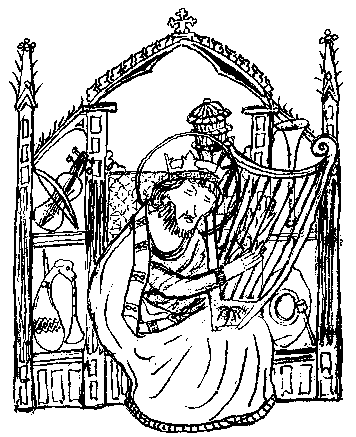
\includegraphics[width=5.75cm]{DavidScan.png} %height ~= 7.06 cm
%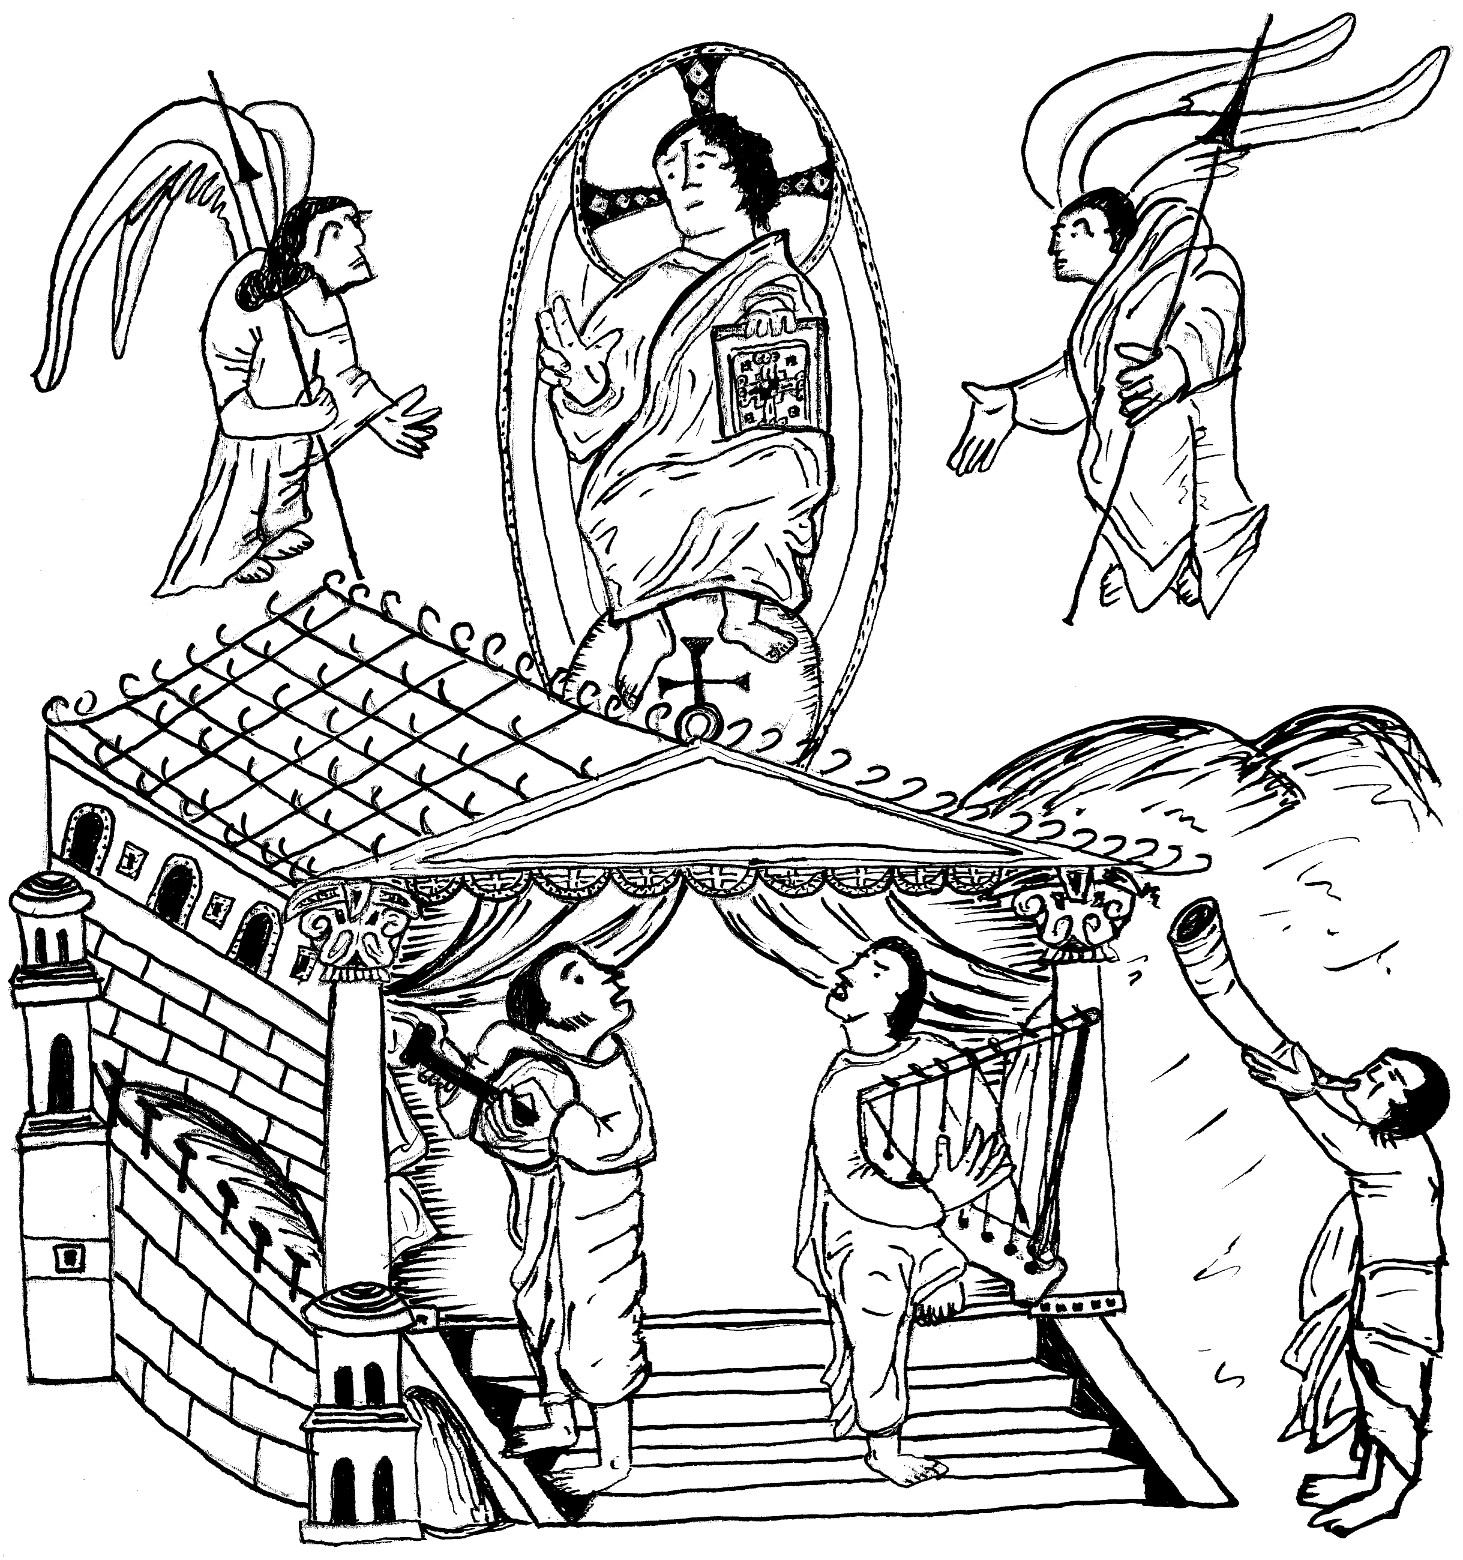
\includegraphics[height=7.06cm]{CoverImage02_s.png}

\includegraphics[height=7.06cm]{David2015.png}

\vspace*{3 mm}

\begin{large}

\textsc{Versio 1.7 MMXV}

\end{large}

\end{center}

%redefine 'plain' page styel to have blue page numbers too
\fancypagestyle{plain}{
	\chead{}
	\cfoot{\textcolor{benblue1}{\thepage}}

}

%\newpage STARTS A NEW PAGE AT THIS POINT
\newpage
\thispagestyle{empty}
\mbox{}
\newpage
\thispagestyle{empty}
\mbox{}
\newpage

\chead{\color{benred8}\textsc{Dominica \textemdash\ Sunday}}
%\cfoot{\thepage}
\cfoot{\textcolor{benblue1}{\thepage}}
\thispagestyle{plain}
%\pagenumbering{roman}  
\pagenumbering{arabic}  
\setcounter{page}{4}


%\pagestyle{plain}

% DOMINICA AD VESPERAS
% START PARALLEL TEXTS
\begin{pages}
\begin{Leftside}
\firstlinenum{10000}\linenumincrement{10000}\beginnumbering\pstart

\begin{center}\begin{Huge}\textsc{\textcolor{benred8}{Dominica ad Vesperas}}\end{Huge}\end{center}

\pend\pstart

\begin{center}Pater no\libertineGlyph{s_t}er. Ave Mar\'{i}a.\end{center}

\pend\pstart

% Here we set the space around the initial.
% Please report to http://home.gna.org/gregorio/gregoriotex/details for more details and options
%was 2.2mm for both
\setspaceafterinitial{2.2mm plus 0em minus 0em}
\setspacebeforeinitial{2.2mm plus 0em minus 0em}

% Here we set the initial font. Change 43 if you want a bigger initial.
\def\greinitialformat#1{%
{\fontsize{43}{43}\selectfont #1}%
}

% We set V/. above the initial.
\gresetfirstlineaboveinitial{\textcolor{benred8}{\small \textsc{\textbf{\Vbar}}}}{\textcolor{benred8}{\small \textsc{\textbf{\Vbar}}}}

% and finally we include the score. The file must be in the same directory as this one.
\includescore{LatinVersion/DeusInAdjutorium.tex}

\pend\pstart

\begin{rubric}
A Septuagesima usque ad Pascha, loco \emph{\textcolor{black}{Allelúia}}, canitur :

\end{rubric}

{\noinitial
\includescore{LatinVersion/LausTibi.tex}
}

\pend\pstart

\vspace{2mm}

\begin{center}\begin{large}\textbf{\textsc{\textcolor{benred8}{1 Antiphona. VII c 2}}}\end{large}\end{center}

\vspace{2mm}

\pend\pstart

% THE BIG INITIAL INSIDE DomAnt1-01.tex
%\raisebox{1.60cm}{\greinitial{D}}%

\def\grebiginitialformat#1{%
{\fontsize{170}{170}\selectfont #1}%
}

{\gresetbiginitial
\includescore{LatinVersion/Dominica/DomAnt1-01_plain_d.tex}

}

\pend\pstart

{
\centering
\textcolor{benred8}{Psalmus 109.}

}

\pend\pstart

\begin{psalmtext}
Donec ponam ini\textbf{mí}cos \textbf{tu}os, \gresixstar\ scabéllum \textbf{pe}dum tu\textbf{ó}rum.

Virgam virtútis tuæ emíttet Dómi\textbf{nus} ex \textbf{Si}on : \gresixstar\ domináre in médio inimi\textbf{có}rum tu\textbf{ó}rum.

Tecum princípium in die virtútis tuæ in splendóri\textbf{bus} sanc\textbf{tó}rum : \gresixstar\ ex útero ante lucíferum \textbf{gé}nu\textbf{i} te.

Jurávit Dóminus et non pæni\textbf{té}bit \textbf{e}um : \gresixstar\ Tu es sacérdos in æt\'{e}rnum secúndum órdi\textbf{nem} Mel\textbf{chí}sedech.

Dóminus a \textbf{dex}tris \textbf{tu}is, \gresixstar\ confrégit in die iræ \textbf{su}æ \textbf{re}ges.

Judicábit in natiónibus, im\textbf{plé}bit ru\textbf{í}nas : \gresixstar\ conquassábit cápita in \textbf{ter}ra mul\textbf{tó}rum.

De torrénte in \textbf{vi}a \textbf{bi}bet : \gresixstar\ proptérea exal\textbf{tá}bit \textbf{ca}put.

Glória \textbf{Pa}tri, et \textbf{Fí}lio, \gresixstar\ et Spi\textbf{rí}tui \textbf{Sanc}to.

Sicut erat in princípio, et \textbf{nunc}, et \textbf{sem}per, \gresixstar\ et in sǽcula sæcu\textbf{ló}rum. \textbf{A}men.

\end{psalmtext}

\pend\pstart

{\noinitial
\includescore{LatinVersion/Dominica/DomAnt1-02.tex}
}

\pend\pstart

%% DOMINICA 2 ANT.

\setspaceafterinitial{6mm plus 0em minus 0em}
\setspacebeforeinitial{6mm plus 0em minus 0em}

\myaboveinitial{2 \Abar\ IV g}
\includescore{LatinVersion/Dominica/DomAnt2-01.tex}

\pend\pstart

{
\centering
\textcolor{benred8}{Psalmus 110.}

}

\pend\pstart

{\noinitial
\includescore{LatinVersion/Dominica/DomFL2.tex}

}

\pend\pstart

\begin{psalmtext}
Magna ó\emph{pera} \textbf{Dó}mini : \gresixstar\ exquisíta in omnes voluntátes \textbf{e}jus.

Conféssio et magnificéntia \emph{opus} \textbf{e}jus : \gresixstar\ et ju\libertineGlyph{s_t}ítia ejus manet in sǽculum \textbf{sǽ}culi.

Memóriam fécit mirabílium suórum, \gredagger\ miséricors et mise\emph{rátor} \textbf{Dó}minus : \gresixstar\ escam dedit timénti\textbf{bus} se.

Memor erit in sǽculum te\libertineGlyph{s_t}a\emph{ménti} \textbf{su}i : \gresixstar\ virtútem óperum suórum annuntiábit pópulo \textbf{su}o :

Ut det illis hæredi\emph{tátem} \textbf{gén}tium : \gresixstar\ ópera mánuum ejus véritas et ju\textbf{dí}cium.

Fidélia ómnia mandáta ejus : \gredagger\ confirmáta in sǽ\emph{culum} \textbf{sǽ}culi : \gresixstar\ fa\libertineGlyph{c_t}a in veritáte et æqui\textbf{tá}te.

Redemptiónem misit pó\emph{pulo} \textbf{su}o : \gresixstar\ mandávit in ætérnum te\libertineGlyph{s_t}améntum \textbf{su}um.

\textcolor{benred8}{\emph{Fit reverentia :}} San\libertineGlyph{c_t}um et terríbile \emph{nomen} \textbf{e}jus : \gresixstar\ inítium sapiéntiae timor \textbf{Dó}mini.

Intellé\libertineGlyph{c_t}us bonus ómnibus facién\emph{tibus} \textbf{e}um : \gresixstar\ laudátio ejus manet in sǽculum \textbf{sǽ}culi.

Glória Pa\emph{tri, et} \textbf{Fí}lio, \gresixstar\ et Spirítui \textbf{Sanc}to.

Sicut erat in princípio, et \emph{nunc, et} \textbf{sem}per, \gresixstar\ et in sǽcula sæculórum. \textbf{A}men.

\end{psalmtext}

\pend\pstart

{\noinitial
\includescore{LatinVersion/Dominica/DomAnt2-02.tex}
}

\pend\pstart

%% DOMINICA 3 ANT.

\setspaceafterinitial{7mm plus 0em minus 0em}
\setspacebeforeinitial{7mm plus 0em minus 0em}

\myaboveinitial{3 \Abar\ IV a}
\includescore{LatinVersion/Dominica/DomAnt3-01.tex}

\pend\pstart

{
\centering
\textcolor{benred8}{Psalmus 111.}

}

\pend\pstart

{\noinitial
\includescore{LatinVersion/Dominica/DomFL3.tex}
}

\pend\pstart

\begin{psalmtext}
Potens in terra erit \emph{semen} \textbf{e}jus : \gresixstar\ generátio re\libertineGlyph{c_t}órum \emph{benedi}\textbf{cé}tur.

Glória et divítiae in \emph{domo} \textbf{e}jus : \gresixstar\ et ju\libertineGlyph{s_t}ítia ejus manet in \emph{sǽculum} \textbf{sǽ}culi.

Exórtum e\libertineGlyph{s_t} in ténebris \emph{lumen} \textbf{rec}tis : \gresixstar\ miséricors, et mise\emph{rátor, et} \textbf{jus}tus.

Jucúndus homo qui miserétur et cómmodat, \gredagger\ dispónet sermónes suos \emph{in ju}\textbf{dí}cio : \gresixstar\ quia in ætérnum \emph{non commo}\textbf{vé}bitur.

In memória ætérna \emph{erit} \textbf{jus}tus : \gresixstar\ ab auditióne ma\emph{la non ti}\textbf{mé}bit.

Parátum cor ejus speráre in Dómino, \gredagger\ confirmátum \emph{e\libertineGlyph{s_t} cor} \textbf{e}jus : \gresixstar\ non commovébitur donec despíciat i\emph{nimícos} \textbf{su}os.

Dispérsit, dedit paupéribus : \gredagger\ ju\libertineGlyph{s_t}ítia ejus manet in sǽ\emph{culum} \textbf{sǽ}culi : \gresixstar\ cornu ejus exaltá\emph{bitur in} \textbf{gló}ria.

Peccátor vidébit, et irascétur, \gredagger\ déntibus suis fremet \emph{et ta}\textbf{bé}scet : \gresixstar\ desidérium pecca\emph{tórum pe}\textbf{rí}bit.

Glória Pa\emph{tri, et} \textbf{Fí}lio, \gresixstar\ et Sp\emph{irítui} \textbf{Sanc}to.

Sicut erat in princípio, et \emph{nunc, et} \textbf{sem}per, \gresixstar\ et in sǽcula sæ\emph{culórum}. \textbf{A}men.

\end{psalmtext}

\pend\pstart

{\noinitial
\includescore{LatinVersion/Dominica/DomAnt3-02.tex}
}

\pend\pstart

%% DOMINICA 4 ANT.

\setspaceafterinitial{7mm plus 0em minus 0em}
\setspacebeforeinitial{7mm plus 0em minus 0em}

\myaboveinitial{4 \Abar\ VII c}
\includescore{LatinVersion/Dominica/DomAnt4-01.tex}

\pend\pstart

{
\centering
\textcolor{benred8}{Psalmus 112.}

}

\pend\pstart

{\noinitial
\includescore{LatinVersion/Dominica/DomFL4.tex}
}

\pend\pstart

\begin{psalmtext}
\textcolor{benred8}{\emph{Fit reverentia :}} Sit nomen Dómini \textbf{be}ne\textbf{díc}tum, \gresixstar\ ex hoc nunc, et \textbf{us}que in \textbf{sǽ}culum.

A solis ortu usque \textbf{ad} oc\textbf{cá}sum, \gresixstar\ laudábile \textbf{no}men \textbf{Dó}mini.

Excélsus super omnes \textbf{gen}tes \textbf{Dó}minus, \gresixstar\ et super cælos \textbf{gló}ria \textbf{e}jus.

Quis sicut Dóminus Deus no\libertineGlyph{s_t}er, qui in \textbf{al}tis \textbf{há}bitat, \gresixstar\ et humília réspicit in cælo \textbf{et} in \textbf{ter}ra?

Súscitans a \textbf{ter}ra \textbf{í}nopem, \gresixstar\ et de \libertineGlyph{s_t}ércore \textbf{é}rigens \textbf{páu}perem :

Ut cóllocet eum \textbf{cum} prin\textbf{cí}pibus, \gresixstar\ cum princípibus \textbf{pó}puli \textbf{su}i.

Qui habitáre facit \libertineGlyph{s_t}éri\textbf{lem} in \textbf{do}mo, \gresixstar\ matrem fili\textbf{ó}rum lae\textbf{tán}tem.

Glória \textbf{Pa}tri, et \textbf{Fí}lio, \gresixstar\ et Spi\textbf{rí}tui \textbf{Sanc}to.

Sicut erat in princípio, et \textbf{nunc}, et \textbf{sem}per, \gresixstar\ et in sǽcula sæcu\textbf{ló}rum. \textbf{A}men.

\end{psalmtext}

\pend\pstart

{\noinitial
\includescore{LatinVersion/Dominica/DomAnt4-02.tex}
}

\pend\pstart

%% DOMINICA 5 ANT.

\setspaceafterinitial{6.5mm plus 0em minus 0em}
\setspacebeforeinitial{6.5mm plus 0em minus 0em}

\myaboveinitial{5 \Abar\ T. Per.}
\includescore{LatinVersion/Dominica/DomAnt5-01.tex}

\pend\pstart

{
\centering
\textcolor{benred8}{Psalmus 113.}

}

\pend\pstart

{\noinitial
\includescore{LatinVersion/Dominica/DomFL5.tex}
}

\pend\pstart

\begin{psalmtext}
Fa\libertineGlyph{c_t}a e\libertineGlyph{s_t} Judǽa san\libertineGlyph{c_t}ifi\emph{cátio} \textbf{e}jus, \gresixstar\ Israel potés\emph{tas} \textbf{e}jus.

Mare \emph{vidit, et} \textbf{fu}git : \gresixstar\ Jordánis convérsus e\libertineGlyph{s_t} \emph{re}\textbf{trór}sum.

Montes exsultavé\emph{runt ut a}\textbf{rí}etes : \gresixstar\ et colles sicut a\emph{gni} \textbf{ó}vium.

Quid e\libertineGlyph{s_t} tibi ma\emph{re quod fu}\textbf{gís}ti? \gresixstar\ et tu Jordánis, quia convérsus es \emph{re}\textbf{trór}sum.

Montes exsultá\libertineGlyph{s_t}is \emph{sicut a}\textbf{rí}etes, \gresixstar\ et colles sicut a\emph{gni} \textbf{ó}vium?

A fácie Dómini \emph{mota e\libertineGlyph{s_t}} \textbf{ter}ra, \gresixstar\ a fácie De\emph{i} \textbf{Ja}cob : 

Qui convértit petram in \emph{\libertineGlyph{s_t}agna a}\textbf{quá}rum, \gresixstar\ et rupem in fontes \emph{a}\textbf{quá}rum.

Non nobis Dó\emph{mine, non} \textbf{no}bis : \gresixstar\ sed nómini tuo \emph{da} \textbf{gló}riam.

Super misericórdia tua et ve\emph{ritáte} \textbf{tu}a : \gresixstar\ nequándo dicant gentes : Ubi e\libertineGlyph{s_t} Deus \emph{e}\textbf{ó}rum?

Deus autem \emph{no\libertineGlyph{s_t}er in} \textbf{cæ}lo : \gresixstar\ ómnia quæcúmque vólu\emph{it}, \textbf{fe}cit.

Simulácra géntium ar\emph{géntum et} \textbf{au}rum, \gresixstar\ ópera mánu\emph{um} \textbf{hó}minum.

Os habent, \emph{et non lo}\textbf{quén}tur : \gresixstar\ óculos habent, et non \emph{vi}\textbf{dé}bunt.

Aures ha\emph{bent, et non} \textbf{áu}dient : \gresixstar\ nares habent, et non o\emph{do}\textbf{rá}bunt.

Manus habent, et non palpábunt : \gredagger\ pedes habent, et \emph{non ambu}\textbf{lá}bunt : \gresixstar\ non clamábunt in gúttu\emph{re} \textbf{su}o.

Símiles illis fiant qui \emph{fáciunt} \textbf{e}a : \gresixstar\ et omnes qui confídunt \emph{in} \textbf{e}is.

Domus Israel spe\emph{rávit in} \textbf{Dó}mino : \gresixstar\ adjútor eórum et proté\libertineGlyph{c_t}or \emph{e}\textbf{ó}rum e\libertineGlyph{s_t}.

Domus Aaron spe\emph{rávit in} \textbf{Dó}mino : \gresixstar\ adjútor eórum et proté\libertineGlyph{c_t}or \emph{e}\textbf{ó}rum e\libertineGlyph{s_t}.

Qui timent Dóminum spera\emph{vérunt in} \textbf{Dó}mino : \gresixstar\ adjútor eórum et proté\libertineGlyph{c_t}or \emph{e}\textbf{ó}rum e\libertineGlyph{s_t}.

Dóminus me\emph{mor fuit} \textbf{nos}tri : \gresixstar\ et benedí\emph{xit} \textbf{no}bis.

Benedíxit \emph{dómui} \textbf{Is}rael : \gresixstar\ benedíxit dómu\emph{i} \textbf{A}aron.

Benedíxit ómnibus \emph{qui timent} \textbf{Dó}minum \gresixstar\ pusíllis cum \emph{ma}\textbf{jór}ibus.

Adjíciat \emph{Dóminus} \textbf{su}per vos : \gresixstar\ super vos, et super fíli\emph{os} \textbf{ves}tros.

Benedíc\emph{ti vos a} \textbf{Dó}mino, \gresixstar\ qui fecit cælum \emph{et} \textbf{ter}ram.

Cæ\emph{lum cæli} \textbf{Dó}mino : \gresixstar\ terram autem dedit fíli\emph{is} \textbf{hó}minum.

Non mórtui lau\emph{dábunt te} \textbf{Dó}mine : \gresixstar\ neque omnes qui descéndunt in \emph{in}\textbf{fér}num.

Sed nos qui vívimus bene\emph{dícimus} \textbf{Dó}mino, \gresixstar\ ex hoc nunc et usque \emph{in} \textbf{sǽ}culum.

Glória \emph{Patri, et} \textbf{Fí}lio, \gresixstar\ et Spirítu\emph{i} \textbf{Sanc}to.

Sicut erat in princípio, \emph{et nunc, et} \textbf{sem}per, \gresixstar\ et in sǽcula sæculó\emph{rum}. \textbf{A}men.

\end{psalmtext}

\pend\pstart

{\noinitial
\includescore{LatinVersion/Dominica/DomAnt5-02.tex}
}

\pend\pstart

\begin{rubric}
Sequens Capitulum \emph{\textcolor{black}{Bened\'{i}\libertineGlyph{c_t}us Deus}} canitur a Dominica II po\libertineGlyph{s_t}  Epiphaniam usque ad Septuagesimam, et a Dominica III po\libertineGlyph{s_t} Penteco\libertineGlyph{s_t}en usque ad Adventum tantum. Hymnus vero canitur in iisdem Dominicis po\libertineGlyph{s_t} Penteco\libertineGlyph{s_t}en et Epiphaniam, etiam usque ad Dominicam I Quadragesim\ae .

\end{rubric}

\pend\pstart

% DOMINICA CAPITULUM

\subsection*{Capitulum.\capitulumSpace \emph{2 Cor. 1, 3--4.}}

\label{DominicaCapitulum}

\pend\pstart


\myaboveinitial{}
\setspaceafterinitial{0mm plus 0em minus 0em}
\setspacebeforeinitial{0mm plus 0em minus 0em}
\includescore{LatinVersion/CapitulumBenedictus.tex}

\color{black}

\pend\pstart

% DOMINICA HYMNUS HIEME

\newpage

\subsection*{Hymnus.\\Tonus in Hieme.}

\pend\pstart

\begin{rubric}
Sequens tonus canitur in Dominicis po\libertineGlyph{s_t} Epiphaniam a die 14 Januarii usque ad Dominicam Quinquagesim\ae\ inclusive, et a Dominica proximiori Kalendis O\libertineGlyph{c_t}obris scilicet a die 28 Septembris usque ad Dominicam ultimam po\libertineGlyph{s_t} Penteco\libertineGlyph{s_t}en.

\end{rubric}

\pend\pstart

\setspaceafterinitial{1mm plus 0em minus 0em}
\setspacebeforeinitial{1mm plus 0em minus 0em}

\myaboveinitial{IV}
\includescore{LatinVersion/Dominica/DomHym-Hieme.tex}

\pend\pstart

\begin{rubric}
Quando fit Commemoratio B. M. V., canitur doxologia \emph{\textcolor{black}{Gl\'{o}ria tibi, D\'{o}mine, Qui natus es de V\'{i}rgine, Cum Patre \emph{et} Sancto Sp\'{i}ritu, In sempit\'{e}rna s\'{\ae}cula}}, sed non mutatur tonus hymni.

\end{rubric}

\pend\pstart

{\noinitial
\includescore{LatinVersion/DirigaturDomine.tex}

}

\begin{response}
\hspace{1.0 mm}\Rbar\ Sicut \hspace{1.1mm} inc\'{e}nsum \hspace{1.1mm} in \hspace{1.1mm} consp\'{e}\libertineGlyph{c_t}u \hspace{1.2mm} tu- o.

\end{response}

\pend\pstart

% DOMINICA HYMNUS AESTATE

\subsection*{Tonus in \AE \libertineGlyph{s_t}ate.}

\pend\pstart

\begin{rubric}
Sequens tonus canitur in Dominica IV et reliquis Dominicis po\libertineGlyph{s_t} Penteco\libertineGlyph{s_t}en usque ad Dominicam proximiorem Kalendis O\libertineGlyph{c_t}obris id e\libertineGlyph{s_t} ad diem 27 Septembris inclusive occurrentibus.

\end{rubric}

\pend\pstart

\myaboveinitial{VIII}
\includescore{LatinVersion/Dominica/DomHym-Aestate.tex}

\pend\pstart

\begin{response}
\Vbar\ Dirig\'{a}tur D\'{o}mine or\'{a}tio mea.\\
\Rbar\ Sicut inc\'{e}nsum in consp\'{e}\libertineGlyph{c_t}u tuo.

\end{response}

\pend\pstart

% DOMINICA HYMNUS AD LIB 1

\subsection*{Tonus ad libitum I.}

\pend\pstart

\myaboveinitial{VIII}
\includescore{LatinVersion/Dominica/DomHym-AdLib1.tex}

\pend\pstart

\begin{response}
\Vbar\ Dirig\'{a}tur D\'{o}mine or\'{a}tio mea.\\
\Rbar\ Sicut inc\'{e}nsum in consp\'{e}\libertineGlyph{c_t}u tuo.

\end{response}

\pend\pstart

% DOMINICA HYMNUS AD LIB 2

\subsection*{Tonus ad libitum II.}

\pend\pstart

\setspaceafterinitial{0mm plus 0em minus 0em}
\setspacebeforeinitial{0mm plus 0em minus 0em}

\myaboveinitial{I}
\includescore{LatinVersion/Dominica/DomHym-AdLib2.tex}

\pend\pstart

\begin{response}
\Vbar\ Dirig\'{a}tur D\'{o}mine or\'{a}tio mea.\\
\Rbar\ Sicut inc\'{e}nsum in consp\'{e}\libertineGlyph{c_t}u tuo.

\end{response}

\pend\endnumbering
\end{Leftside}
%%%%%%%%%%%%%%%%%%%%%%%%%%%%%%%%%%%%%%%%%%%%%%%%%%%%%%
%%%%%%%%%%%%%%%%%%%%%%%%%%%%%%%%%%%%%%%%%%%%%%%%%%%%%%
\begin{Rightside}

\firstlinenum{10000}\linenumincrement{10000}\beginnumbering\pstart



% SUNDAY AT VESPERS

\begin{center}\begin{Huge}\textsc{\textcolor{benred8}{Sunday at Vespers}}\end{Huge}\end{center}

\pend\pstart

\begin{center}Our Father. Hail Mary.\end{center}

\pend\pstart

%\setspaceafterinitial{2.2mm plus 0em minus 0em}
%\setspacebeforeinitial{2.2mm plus 0em minus 0em}

\setspaceafterinitial{0mm plus 0em minus 0em}
\setspacebeforeinitial{0mm plus 0em minus 0em}

\def\greinitialformat#1{%
{\fontsize{43}{43}\selectfont #1}%
}

\myaboveinitial{\Vbar\ \ \ }
\includescore{EnglishVersion/DeusInAdjutorium.tex}

\pend\pstart

\begin{rubric}
The following is sung from Septuagesima Sunday until Easter in place of \emph{\textcolor{black}{Alleluia}} :

\end{rubric}

{\noinitial
\includescore{EnglishVersion/LausTibi.tex}

}

\pend\pstart

\vspace{2mm}

\begin{center}\begin{large}\textbf{\textsc{\textcolor{benred8}{1 Antiphon. VII c 2}}}\end{large}\end{center}

\vspace{2mm}

\pend\pstart

\def\grebiginitialformat#1{%
{\fontsize{170}{170}\selectfont #1}%
}

{\gresetbiginitial
\includescore{EnglishVersion/Dominica/DomAnt1-01_plain_d.tex}

}

\pend\pstart

{
\centering
\textcolor{benred8}{Psalm 109.}

}

\pend\pstart

\begin{psalmtext}
%The Lord \textbf{said} to \textbf{my} Lord: \gresixstar\ Sit thou \textbf{at} my \textbf{right} hand:

%Until I \textbf{make} thy \textbf{e}nemies \gresixstar\ thy \textbf{foot}stool.

The Lord will send forth the sceptre of thy power \pipe\ out of Sion: \gresixstar\ rule thou in the \pipe\ midst \uline{of~thy}\hspace{2mm}\uline{ene}mies.

With thee is the principality in the day of thy strength: in the \pipe\ brightness \uline{of the} saints: \gresixstar\ from the womb before the day star \pipe\ I begot thee.

The Lord hath sworn, and \pipe\ he will \uline{not re}pent: \gresixstar\ Thou art a priest for ever according to the order \pipe\ of Mel\uline{chise}dech.

The Lord \pipe\ at thy right hand \gresixstar\ hath broken kings in the \pipe\ \textbf{day} \uline{of his} wrath.

He shall judge among nations, \pipe\ he \uline{shall fill} ruins: \gresixstar\ he shall crush the heads in the \pipe\ land of many.

He shall drink of the \pipe\ torrent \uline{in the} way: \gresixstar\ therefore shall he \pipe\ \textbf{lift} \uline{up the} head.

Glory be to the \pipe\ Fa\uline{ther, and}\hspace{2mm}\uline{to the} Son, \gresixstar\ and to the \pipe\ Holy Spirit.

As it was in the beginning, is now, and \pipe\ ever shall be, \gresixstar\ world without \pipe\ \textbf{end}. Amen.

\end{psalmtext}

\pend\pstart

{\noinitial
\includescore{EnglishVersion/Dominica/DomAnt1-02.tex}
}

\pend\pstart

%% SUNDAY 2 ANT.

\setspaceafterinitial{6mm plus 0em minus 0em}
\setspacebeforeinitial{6mm plus 0em minus 0em}

\myaboveinitial{2 \Abar\ IV g}
\includescore{EnglishVersion/Dominica/DomAnt2-01.tex}

\pend\pstart

{
\centering
\textcolor{benred8}{Psalm 110.}

}

\pend\pstart

{\noinitial
\includescore{EnglishVersion/Dominica/DomFL2.tex}

}

\pend\pstart

\begin{psalmtext}
%I will praise thee, O Lord, \emph{with my} \textbf{whole} heart ; \gresixstar\ in the council of the just, and in the congre\textbf{ga}tion.

Great are \pipe\ the \textbf{works} \uline{of the} Lord: \gresixstar\ sought out according to all \pipe\ his wills.

His work is \pipe\ praise and magni\uline{ficence}: \gresixstar\ and his justice continueth for ever and \pipe\ ever.

He hath made a remembrance of his wonderful works, \gredagger\ being a mer- \pipe\ ciful and gra\uline{cious~Lord}:~\gresixstar\ he hath given food to them that \pipe\ fear him.

He will be mindful for e- \pipe\ ver of his co\uline{venant}: \gresixstar\ he will shew forth to his people the power of \pipe\ his works.

That he may give them the inheri- \pipe\ tance of the Gentiles: \gresixstar\ the works of his hands are truth and \pipe\ judgment.

All his commandments are faithful: \gredagger\ confirmed for \pipe\ ever and ever, \gresixstar\ made in truth and \pipe\ e\uline{quity}.

He hath sent redemp- \pipe\ tion to his people: \gresixstar\ he hath commanded his covenant for \pipe\ ever.

\textcolor{benred8}{\emph{A sign of reverence is made:}} Holy and terri- \pipe\ ble \textbf{is} his name : \gresixstar\ the fear of the Lord is the beginning of \pipe\ wisdom.

A good understanding \pipe\ to all that do it: \gresixstar\ his praise continueth for ever and \pipe\ ever.

Glory be to the Father, \pipe\ and \textbf{to} the Son, \gresixstar\ and to the Holy \pipe\ Spirit.

As it was in the beginning, is now, \pipe\ and ever shall be, \gresixstar\ world without end. \pipe\ Amen.

\end{psalmtext}

\pend\pstart

{\noinitial
\includescore{EnglishVersion/Dominica/DomAnt2-02.tex}
}

\pend\pstart

 %% SUNDAY 3 ANT.

\setspaceafterinitial{5mm plus 0em minus 0em}
\setspacebeforeinitial{5mm plus 0em minus 0em}

\myaboveinitial{3 \Abar\ IV a}
\includescore{EnglishVersion/Dominica/DomAnt3-01.tex}

\pend\pstart

{
\centering
\textcolor{benred8}{Psalm 111.}

}

\pend\pstart

{\noinitial
\includescore{EnglishVersion/Dominica/DomFL3.tex}
}

\pend\pstart

\begin{psalmtext}
%Blessed is the man that \emph{feareth} \textbf{the} Lord: \gresixstar\ he shall delight exceedingly \emph{in his com}\textbf{mand}ments.

His seed shall be \pipe\ migh\uline{ty up}\textbf{on} earth: \gresixstar\ the generation of the right- \pipe\ eous \textbf{shall} be \uline{blessed}.

Glory and wealth shall \pipe\ be \textbf{in} his house: \gresixstar\ and his justice remaineth for \pipe\ \textbf{e}ver and \uline{ever}.

To the righteous a light is \pipe\ risen up in \uline{darkness}: \gresixstar\ he is merciful, and com- \pipe\ passionate and just.

Acceptable is the man that sheweth mercy and lendeth: \gredagger\ he shall or- \pipe\ der his words with \uline{judgment}: \gresixstar\ because he shall not \pipe\ be \textbf{moved} for \uline{ever}.

The just shall be in ever- \pipe\ \textbf{last}ing re\underline{membrance}: \gresixstar\ he shall not fear \pipe\ the \textbf{e}vil \uline{hearing}.

His heart is ready to hope in the Lord: \gredagger\ \pipe\ his \textbf{heart} is \uline{strengthened}, \gresixstar\ he shall not be moved until he look \pipe\ over his e\uline{nemies}.

He hath distributed, he hath given to the poor: \gredagger\ his justice remaineth \pipe\ for ever and \uline{ever}: \gresixstar\ his horn shall be ex- \pipe\ \textbf{al}ted in \uline{glory}.

The wicked shall see, and shall be angry, \gredagger\ he shall gnash with his \pipe\ \uline{\textbf{teeth} and}\hspace{2mm}\uline{\textbf{pine} a}way: \gresixstar\ the desire of the \pipe\ \textbf{wi}cked shall \uline{perish}.

Glory be to the Father, \pipe\ and \textbf{to} the Son, \gresixstar\ and to the \pipe\ \textbf{Holy} \uline{Spirit}.

As it was in the beginning, is now, \pipe\ and ever shall be, \gresixstar\ world \pipe\ \uline{without} \textbf{end}. Amen.

\end{psalmtext}

\pend\pstart

{\noinitial
\includescore{EnglishVersion/Dominica/DomAnt3-02.tex}
}

\pend\pstart

%% SUNDAY 4 ANT.

\setspaceafterinitial{7mm plus 0em minus 0em}
\setspacebeforeinitial{7mm plus 0em minus 0em}

\myaboveinitial{4 \Abar\ VII c}
\includescore{EnglishVersion/Dominica/DomAnt4-01.tex}

\pend\pstart

{
\centering
\textcolor{benred8}{Psalm 112.}

}

\pend\pstart

{\noinitial
\includescore{EnglishVersion/Dominica/DomFL4.tex}
}

\pend\pstart

\begin{psalmtext}
%Praise the \textbf{Lord}, ye \textbf{child}ren: \gresixstar\ praise ye the \textbf{name} of \textbf{the} Lord.

\textcolor{benred8}{\emph{A sign of reverence is made:}} Blessed be the \pipe\ \textbf{name} \uline{of the} Lord, \gresixstar\ from henceforth \pipe\ now \uline{and for} ever.

From the rising of the sun unto the going \pipe\ \textbf{down} \uline{of the} same, \gresixstar\ the name of the Lord is \pipe\ \textbf{worth}\uline{y of} praise.

The Lord is high a- \pipe\ bove all nations; \gresixstar\ and his glory a- \pipe\ bove the heavens.

Who is as the Lord our God, who \pipe\ \textbf{dwel}\uline{leth on} high: \gresixstar\ and looketh down on the low things in \pipe\ heaven \uline{and in} earth?

Raising up the \pipe\ needy \uline{from the} earth, \gresixstar\ and lifting up the poor \pipe\ out \uline{of the} dunghill:

That he may \pipe\ place \uline{him with} princes, \gresixstar\ with the princes \pipe\ of his people.

Who maketh a barren woman to \pipe\ \textbf{dwell} \uline{in a} house, \gresixstar\ the joyful \pipe\ mo\uline{ther of} children.

Glory be to the \pipe\ Fa\uline{ther, and}\hspace{2mm}\uline{to the} Son, \gresixstar\ and to the \pipe\ Holy Spirit.

As it was in the beginning, is now, and \pipe\ ever shall be, \gresixstar\ world without \pipe\ \textbf{end}. Amen.

\end{psalmtext}

\pend\pstart

{\noinitial
\includescore{EnglishVersion/Dominica/DomAnt4-02.tex}
}

\pend\pstart

%% SUNDAY 5 ANT.

\setspaceafterinitial{6.5mm plus 0em minus 0em}
\setspacebeforeinitial{6.5mm plus 0em minus 0em}

\myaboveinitial{5 \Abar\ Per. T.}
\includescore{EnglishVersion/Dominica/DomAnt5-01.tex}

\pend\pstart

{
\centering
\textcolor{benred8}{Psalm 113.}

}

\pend\pstart

{\noinitial
\includescore{EnglishVersion/Dominica/DomFL5.tex}
}

\pend\pstart

\begin{psalmtext}
%When Isra- \pipe\ el went out of Egypt, \gresixstar\ the house of Jacob from a \pipe\ bar\uline{barous} people:

Judea was \pipe\ made his sanctuary, \gresixstar\ Israel \pipe\ his dominion.

The \pipe\ \textbf{sea} saw and \textbf{fled}: \gresixstar\ Jor- \pipe\ dan was turned back.

The \pipe\ mountains skipped like \textbf{rams}, \gresixstar\ and the hills like the \pipe\ \textbf{lambs} \uline{of the} flock.

What ailed thee, O thou \pipe\ sea, that thou didst \textbf{flee}: \gresixstar\ and thou, O Jordan, that \pipe\ thou wast turned back?

Ye mountains, \pipe\ that ye skipped like \textbf{rams}, \gresixstar\ and ye hills, like \pipe\ \textbf{lambs} \uline{of the} flock?

At the presence of the \pipe\ Lord the earth was \textbf{moved}, \gresixstar\ at the presence of the \pipe\ \uline{\textbf{God}~of} Jacob:

Who turned the \pipe\ rock \uline{into} pools of water, \gresixstar\ and the stony hill into \pipe\ foun\uline{tains of} waters.

Not to us, O \pipe\ \textbf{Lord}, not to \textbf{us}; \gresixstar\ but to thy \pipe\ \uline{\textbf{name} give} glory.

For thy mer- \pipe\ cy, and for thy truth's sake: \gresixstar\ lest the Gentiles should say: \pipe\ \uline{\textbf{Where} is} their God?

But our \pipe\ \textbf{God} is in heaven: \gresixstar\ he hath done all things whatso- \pipe\ ever he would.

The idols of the \pipe\ Gen\uline{tiles are} sil\uline{ver and} \textbf{gold}, \gresixstar\ the \pipe\ works \uline{of the} \uline{hands of} men.

They have \pipe\ mouths and \textbf{speak not}: \gresixstar\ they have \pipe\ eyes and see not.

They have \pipe\ ears and \textbf{hear not}: \gresixstar\ they have \pipe\ no\uline{ses and} smell not.

They have hands and feel not: \gredagger\ they have \pipe\ feet and \textbf{walk not}: \gresixstar\ neither shall they \pipe\ cry~\uline{out~through} their throat.

Let them that make them be- \pipe\ come like unto \textbf{them}: \gresixstar\ and all \pipe\ such as \uline{trust in} them.

The house of Israel hath \pipe\ \textbf{hoped} in the \textbf{Lord}: \gresixstar\ he is their helper and \pipe\ their protector.

The house of Aaron hath \pipe\ \textbf{hoped} in the \textbf{Lord}: \gresixstar\ he is their helper and \pipe\ their protector.

They that fear the Lord have \pipe\ \textbf{hoped} in the \textbf{Lord}: \gresixstar\ he is their helper and \pipe\ their protector.

The Lord \pipe\ hath been mindful of us, \gresixstar\ \pipe\ and hath blessed us.

He hath \pipe\ blessed the house of Is\uline{rael}: \gresixstar\ he hath blessed the \pipe\ house of Aaron.

He hath blessed \pipe\ all that fear the \textbf{Lord}, \gresixstar\ both \pipe\ little and great.

May the Lord add \pipe\ \textbf{bles}sings upon you: \gresixstar\ upon you, and u- \pipe\ pon your children.

Blessed \pipe\ be you of the \textbf{Lord}, \gresixstar\ who made \pipe\ heaven and earth.

The heaven of \pipe\ heaven is the \textbf{Lord's}: \gresixstar\ but the earth he has given to the \pipe\ children of men.

The dead shall not \pipe\ \textbf{praise} thee, O \textbf{Lord}: \gresixstar\ nor any of them that \pipe\ go down to hell.

But we that \pipe\ \textbf{live} bless the \textbf{Lord}: \gresixstar\ from this time \pipe\ now \uline{and for} ever.

Glory be to the \pipe\ Fa\uline{ther, and} to the \textbf{Son}, \gresixstar\ and to the \pipe\ Holy Spirit.

As it was in the beginning, is \pipe\ now, and ever shall be, \gresixstar\ world with- \pipe\ out end. Amen.

\end{psalmtext}

\pend\pstart

{\noinitial
\includescore{EnglishVersion/Dominica/DomAnt5-02.tex}
}

\pend\pstart

\begin{rubric}
The following Chapter \emph{\textcolor{black}{Blessed be the God}} is only sung from the Second Sunday after Epiphany until Septuagesima Sunday and from the Third Sunday after Pentecost until Advent. The Hymn is sung on those same Sundays, but also continues until the First Sunday of Lent.

\end{rubric}

\pend\pstart

% SUNDAY CHAPTER

\subsection*{Chapter.\capitulumSpace \emph{2 Cor. 1, 3--4.}}

\label{SundayChapter}

\pend\pstart

\myaboveinitial{}
\setspaceafterinitial{0mm plus 0em minus 0em}
\setspacebeforeinitial{0mm plus 0em minus 0em}
\includescore{EnglishVersion/CapitulumBenedictus.tex}

\color{black}

\pend\pstart

% SUNDAY WINTER HYMN

\newpage

\subsection*{Hymn.\\Winter Tone.}

\pend\pstart

\begin{rubric}
The following tone is sung on Sundays after Epiphany between and including the 14\textsuperscript{th} of January and Quinqugesima Sunday. It is also sung from the Sunday nearest to the 1\textsuperscript{st} of October (the first Sunday on or after the 28\textsuperscript{th} of September) until the last Sunday after Pentecost.

\end{rubric}

\pend\pstart

\setspaceafterinitial{0mm plus 0em minus 0em}
\setspacebeforeinitial{0.8mm plus 0em minus 0em}

\myaboveinitial{IV}
\includescore{EnglishVersion/Dominica/DomHym-Hieme.tex}

\pend\pstart

\begin{rubric}
When a Commemoration is made of the Blessed Virgin Mary, a different Doxology is sung for the Hymn, namely, \emph{\textcolor{black}{O Jesu, born of Virgin bright, Immortal glory be to thee; Praise to the Father infinite, And Holy Ghost eternally}}. This is sung to the same tone.

\end{rubric}

\pend\pstart

{\noinitial
\includescore{EnglishVersion/DirigaturDomine.tex}

}

\begin{response}
\hspace{1.0 mm}\Rbar\ As \hspace{1.1mm} incense \hspace{1.1mm} in \hspace{1.5mm} thy \hspace{1.2mm} sight.

\end{response}

\pend\pstart

% SUNDAY SUMMER HYMN

\subsection*{Summer Tone.}

\pend\pstart

\begin{rubric}
The following tone is sung from the Fourth Sunday after Pentecost until the Sunday nearest to the 1\textsuperscript{st} of October (any Sundays up to and including the 27\textsuperscript{th} of September).

\end{rubric}

\pend\pstart

\setspaceafterinitial{0mm plus 0em minus 0em}
\setspacebeforeinitial{0.8mm plus 0em minus 0em}

\myaboveinitial{VIII}
\includescore{EnglishVersion/Dominica/DomHym-Aestate.tex}

\pend\pstart

\begin{response}
\Vbar\ O Lord, direct my prayer.\\
\Rbar\ As incense in thy sight.

\end{response}

\pend\pstart

% SUNDAY HYMN AD LIB 1

\subsection*{\emph{Ad libitum} Tone I.}

\pend\pstart

\setspaceafterinitial{0mm plus 0em minus 0em}
\setspacebeforeinitial{0.8mm plus 0em minus 0em}

\myaboveinitial{VIII}
\includescore{EnglishVersion/Dominica/DomHym-AdLib1.tex}

\pend\pstart

\begin{response}
\Vbar\ O Lord, direct my prayer.\\
\Rbar\ As incense in thy sight.

\end{response}

\pend\pstart

% SUNDAY HYMN AD LIB 2

\subsection*{\emph{Ad libitum} Tone II.}

\pend\pstart

\setspaceafterinitial{0mm plus 0em minus 0em}
\setspacebeforeinitial{0mm plus 0em minus 0em}

\myaboveinitial{I}
\includescore{EnglishVersion/Dominica/DomHym-AdLib2.tex}

\pend\pstart

\begin{response}
\Vbar\ O Lord, direct my prayer.\\
\Rbar\ As incense in thy sight.

\end{response}

\pend\endnumbering
\end{Rightside}
\end{pages}
\Pages

%%%%%%%%%%%%%%%%%%%%%%%%%%%%%%%%%%%%%%%%%%%%%%%%%%%%%%
%%%%%%%%%%%%%%%%%%%%%%%%%%%%%%%%%%%%%%%%%%%%%%%%%%%%%%

\begin{pages}
\begin{Leftside}
\firstlinenum{10000}\linenumincrement{10000}\beginnumbering\pstart

% DOMINICA MAGNIFICAT

\subsection*{Canticum Beat\ae\ Mari\ae\ Virginis.\capitulumSpace \emph{Luc. 1, 46--55.}}

\pend\pstart

\begin{rubric}
Canitur Antiphona propria.

\end{rubric}

\pend\pstart

\begin{psalmtext}
\lettrine[lhang=0.70]{M}{a}gn\'{i}ficat \grealtcross\ \'{a}nima mea D\'{o}minum :
%Magn\'{i}ficat \gresixstar\ \'{a}nima mea D\'{o}minum :

\hspace*{9.5 mm}Et exsult\'{a}vit sp\'{i}ritus meus \gresixstar\ in Deo salut\'{a}ri meo.

Quia resp\'{e}xit humilit\'{a}tem anc\'{i}ll\ae\ su\ae\ : \gresixstar\ ecce enim ex hoc be\'{a}tam me dicent omnes generati\'{o}nes.

Quia fecit mihi magna qui potens e\libertineGlyph{s_t} : \gresixstar\ et san\libertineGlyph{c_t}um nomen ejus.

Et miseric\'{o}rdia ejus a prog\'{e}nie in prog\'{e}nies \gresixstar\ tim\'{e}ntibus eum.

Fecit pot\'{e}ntiam in br\'{a}chio suo : \gresixstar\ disp\'{e}rsit sup\'{e}rbos mente cordis sui.

Dep\'{o}suit pot\'{e}ntes de sede, \gresixstar\ et exalt\'{a}vit h\'{u}miles.

Esuri\'{e}ntes impl\'{e}vit bonis : \gresixstar\ et d\'{i}vites dim\'{i}sit in\'{a}nes.

Susc\'{e}pit Israel p\'{u}erum suum, \gresixstar\ record\'{a}tus miseric\'{o}rdi\ae\ su\ae.

Sicut loc\'{u}tus e\libertineGlyph{s_t} ad patres nostros, \gresixstar\ Abraham, et s\'{e}mini ejus in s\'{\ae}cula.

Glória Patri, et Fílio, \gresixstar\ et Spirítui San\libertineGlyph{c_t}o.

Sicut erat in princípio, et nunc, et semper, \gresixstar\ et in sǽcula sæculórum. Amen.

\end{psalmtext}

\pend\pstart

\begin{rubric}
Deinde repetitur Antiphona.

\end{rubric}

\pend\pstart

\subsection*{Oratio.}

\pend\pstart

\setspaceafterinitial{1.2mm plus 0em minus 0em}
\setspacebeforeinitial{1.2mm plus 0em minus 0em}

\myaboveinitial{\Vbar}
\includescore{LatinVersion/DomineExaudi-short-01.tex}

\pend\pstart

\begin{rubric}
Canitur Oratio propria, secundum tonum ut habetur in p.~\pageref{sec:TonusOrationis}, et post eam, si occurrat eo die aliquod Fe\libertineGlyph{s_t}um Simplex, vel ad modum Simplicis recolendum, fit de eo commemoratio. Po\libertineGlyph{s_t}remo (~si id tempus requirit~) fiunt Commemorationes de San\libertineGlyph{c_t}a Maria, de San\libertineGlyph{c_t}o Joseph, de Apo\libertineGlyph{s_t}olis, et de Patrono Ecclesi\ae\ in ordine aliarum Commemorationum secundum illius dignitatem, et ultimo loco de Pace, ut infra in p.~\pageref{sec:Commem}. Post ultimam Orationem canitur :

\end{rubric}

\pend\pstart

\myaboveinitial{\Vbar}
\includescore{LatinVersion/DomineExaudi-short-01.tex}

\pend\pstart

\begin{rubric}
Per annum :

\end{rubric}

\pend\pstart

\setspaceafterinitial{2.2mm plus 0em minus 0em}
\setspacebeforeinitial{2.2mm plus 0em minus 0em}

\myaboveinitial{I}
\includescore{LatinVersion/Dominica/DomBenedicamus.tex}

\pend\pstart

\begin{rubric}
Tempore Adventus et Quadragesim\ae\ :

\end{rubric}

\pend\pstart

\setspaceafterinitial{2.2mm plus 0em minus 0em}
\setspacebeforeinitial{2.2mm plus 0em minus 0em}

\myaboveinitial{IV}
\includescore{LatinVersion/Dominica/DomBenedicamusAdvLent.tex}

\pend\pstart

\setspaceafterinitial{2.2mm plus 0em minus 0em}
\setspacebeforeinitial{2.2mm plus 0em minus 0em}

\myaboveinitial{\Vbar}
\includescore{LatinVersion/FideliumAnimae.tex}

\pend\pstart

\begin{rubric}
Si po\libertineGlyph{s_t} Vesperas immediate sequatur Completorium, di\libertineGlyph{c_t}o \Vbar\ \emph{\textcolor{black}{Fid\'{e}lium \'{a}nim\ae}}, \libertineGlyph{s_t}atim incipitur \Vbar\ \emph{\textcolor{black}{Jube D\'{o}mine bened\'{i}cere}}. Secus autem, si tunc terminetur Officium, dicitur \emph{\textcolor{black}{Pater no\libertineGlyph{s_t}er}} totum secreto. %Oratione Dominica secreto recitata, dicitur : %, ut infra ad Completorium.

\end{rubric}

\pend\endnumbering
\end{Leftside}
%%%%%%%%%%%%%%%%%%%%%%%%%%%%%%%%%%%%%%%%%%%%%%%%%%%%%%
%%%%%%%%%%%%%%%%%%%%%%%%%%%%%%%%%%%%%%%%%%%%%%%%%%%%%%
\begin{Rightside}

\firstlinenum{10000}\linenumincrement{10000}\beginnumbering\pstart

% SUNDAY MAGNIFICAT

\subsection*{Canticle of the Blessed Virgin Mary.\capitulumSpace \emph{Luke 1, 46--55.}}

\pend\pstart

\begin{rubric}
The antiphon for the Sunday is sung.

\end{rubric}

\pend\pstart

\begin{psalmtext}
\lettrine[lhang=0.70]{M}{y} soul \grealtcross\ doth magnify the Lord.

\hspace*{9.5 mm}And my spirit hath rejoiced \gresixstar\ in God my Saviour.

Because he hath regarded the humility of his handmaid; \gresixstar\ for behold from henceforth all generations shall call me blessed.

Because he that is mighty, hath done great things to me; \gresixstar\ and holy is his name.

And his mercy is from generation unto generations, \gresixstar\ to them that fear him.

He hath shewed might in his arm: \gresixstar\ he hath scattered the proud in the conceit of their heart.

He hath put down the mighty from their seat, \gresixstar\ and hath exalted the humble.

He hath filled the hungry with good things; \gresixstar\ and the rich he hath sent empty away.

He hath received Israel his servant, \gresixstar\ being mindful of his mercy:

As he spoke to our fathers, \gresixstar\ to Abraham and to his seed for ever.

Glory be to the Father, and to the Son, \gresixstar\ and to the Holy Spirit.

As it was in the beginning, is now, and ever shall be, \gresixstar\ world without end. Amen.

\end{psalmtext}

\pend\pstart

\begin{rubric}
The Antiphhon is now repeated.

\end{rubric}

\pend\pstart

\subsection*{Oration.}

\pend\pstart

\setspaceafterinitial{1.2mm plus 0em minus 0em}
\setspacebeforeinitial{1.2mm plus 0em minus 0em}

\myaboveinitial{\Vbar}
\includescore{EnglishVersion/DomineExaudi-short-01.tex}

\pend\pstart

\begin{rubric}
The Oration for the Sunday is sung to the tone given on p.~\pageref{sec:TonusOrationis}, and after that if any Simple Feast falls on the same day, its commemoration is sung next. Finally, the Commorations on p.~\pageref{sec:Commem} are sung, with the Commemorations of Saint Mary, Saint Joseph, the Apostles, and the Patron of the Church in order of their dignity and the Commemoration of Peace taking last place. After this final Oration the following is repeated:

\end{rubric}

\pend\pstart

\myaboveinitial{\Vbar}
\includescore{EnglishVersion/DomineExaudi-short-01.tex}

\pend\pstart

\begin{rubric}
Throughout the year:

\end{rubric}

\pend\pstart

\setspaceafterinitial{0mm plus 0em minus 0em}
\setspacebeforeinitial{0mm plus 0em minus 0em}

\myaboveinitial{I}
\includescore{EnglishVersion/Dominica/DomBenedicamus.tex}

\pend\pstart

\begin{rubric}
During Advent and Lent:

\end{rubric}

\pend\pstart

\setspaceafterinitial{0mm plus 0em minus 0em}
\setspacebeforeinitial{0mm plus 0em minus 0em}

\myaboveinitial{IV}
\includescore{EnglishVersion/Dominica/DomBenedicamusAdvLent.tex}

\pend\pstart

\setspaceafterinitial{0mm plus 0em minus 0em}
\setspacebeforeinitial{0mm plus 0em minus 0em}

\myaboveinitial{\Vbar}
\includescore{EnglishVersion/FideliumAnimae.tex}

\pend\pstart

\begin{rubric}
If Compline follows Vespers, \emph{\textcolor{black}{Grant, Lord, a blessing}} is sung straightaway after \emph{\textcolor{black}{May the souls of the faithful}} has finished. Otherwise, if the Office finishes here, a silent \emph{\textcolor{black}{Our Father}} is said.

\end{rubric}

\pend\endnumbering
\end{Rightside}
\end{pages}
\Pages

%%%%%%%%%%%%%%%%%%%%%%%%%%%%%%%%%%%%%%%%%%%%%%%%%%%%%%
%%%%%%%%%%%%%%%%%%%%%%%%%%%%%%%%%%%%%%%%%%%%%%%%%%%%%%
%%%%%%%%%%%%%%%%%%%%%%%%%%%%%%%%%%%%%%%%%%%%%%%%%%%%%%

\begin{pages}
\begin{Leftside}
\firstlinenum{10000}\linenumincrement{10000}\beginnumbering\pstart

% FERIA SECUNDA AD VESPERAS

\section*{Feria Secunda ad Vesperas}

\pend\pstart

\begin{center}Pater no\libertineGlyph{s_t}er. Ave Mar\'{i}a.\end{center}

\pend\pstart

\chead{\color{benred8}\textsc{Feria II \textemdash\ Monday}}
\thispagestyle{plain}

\begin{response}\lettrine{D}{e}us \grealtcross\ in adjut\'{o}rium meum int\'{e}nde. \Rbar\ D\'{o}mine ad adjuv\'{a}ndum me fe\libertineGlyph{s_t}\'{i}na. Gl\'{o}ria Patri, et F\'{i}lio, et Spir\'{i}tui San\libertineGlyph{c_t}o. Sicut erat in princ\'{i}pio, et nunc, et semper, et in s\'{\ae}cula s\ae cul\'{o}rum. Amen. Allel\'{u}ia. \vel\ Laus tibi D\'{o}mine Rex \ae t\'{e}rn\ae\ gl\'{o}ri\ae .

\end{response}

\pend\pstart

% FERIA II 1 ANT

\setspaceafterinitial{7mm plus 0em minus 0em}
\setspacebeforeinitial{7mm plus 0em minus 0em}

\def\greinitialformat#1{%
{\fontsize{60}{60}\selectfont #1}%
}

\myaboveinitial{1 \Abar\ I g 2}
\includescore{LatinVersion/F2/F2Ant1-01.tex}

\pend\pstart

\def\greinitialformat#1{%
{\fontsize{43}{43}\selectfont #1}%
}

{
\centering
\textcolor{benred8}{Psalmus 114.}

}

\pend\pstart

{\noinitial
\includescore{LatinVersion/F2/F2FL1.tex}
}

\pend\pstart

\begin{psalmtext}
Quia inclinávit aurem \textbf{su}am \textbf{mi}hi : \gresixstar\ et in diébus meis \emph{invo}\textbf{cá}bo.

Circumdedérunt me do\textbf{ló}res \textbf{mor}tis : \gresixstar\ et perícula inférni \emph{inve}\textbf{né}runt me.

Tribulatiónem et do\textbf{ló}rem in\textbf{vé}ni : \gresixstar\ et nomen Dómini \emph{invo}\textbf{cá}vi.

O Dómine líbera ánimam meam : \gredagger\ miséricors Dómi\textbf{nus}, et \textbf{jus}tus, \gresixstar\ et Deus no\libertineGlyph{s_t}er \emph{mise}\textbf{ré}tur.

Cu\libertineGlyph{s_t}ódiens \textbf{pár}vulos \textbf{Dó}minus : \gresixstar\ humiliátus sum, et \emph{libe}\textbf{rá}vit me.

Convértere ánima mea in \textbf{ré}quiem \textbf{tu}am : \gresixstar\ quia Dóminus bene\emph{fécit} \textbf{ti}bi.

Quia erípuit ánimam meam de morte : \gredagger\ óculos \textbf{me}os a \textbf{lác}rimis, \gresixstar\ pedes me\emph{os a} \textbf{lap}su.

Pla\textbf{cé}bo \textbf{Dó}mino \gresixstar\ in regió\emph{ne vi}\textbf{vó}rum.

Glória \textbf{Pat}ri, et \textbf{Fí}lio, \gresixstar\ et Spirí\emph{tui} \textbf{Sanc}to.

Sicut erat in princípio, et \textbf{nunc}, et \textbf{sem}per, \gresixstar\ et in sǽcula sæcu\emph{lórum}. \textbf{A}men.

\end{psalmtext}

\pend\pstart

{\noinitial
\includescore{LatinVersion/F2/F2Ant1-02.tex}

}

\pend\pstart

% FERIA II 2 ANT

\setspaceafterinitial{6.5mm plus 0em minus 0em}
\setspacebeforeinitial{6.5mm plus 0em minus 0em}

\myaboveinitial{2 \Abar\ VIII a}
\includescore{LatinVersion/F2/F2FL2.tex}

\pend\pstart

{
\centering
\textcolor{benred8}{Psalmus 115.}

}

\pend\pstart

\begin{psalmtext}
Ego dixi in excéssu \textbf{me}o : \gresixstar\ Omnis \emph{homo} \textbf{men}dax.

Quid retríbuam \textbf{Dó}mino, \gresixstar\ pro ómnibus quæ retrí\emph{buit} \textbf{mi}hi?

Cálicem salutáris ac\textbf{cí}piam : \gresixstar\ et nomen Dómini \emph{invo}\textbf{cá}bo.

Vota mea Dómino reddam coram omni pópulo \textbf{e}jus : \gresixstar\ pretiósa in conspé\libertineGlyph{c_t}u Dómini mors sanc\emph{tórum} \textbf{e}jus :

O Dómine quia ego servus \textbf{tu}us : \gresixstar\ ego servus tuus, et fílius an\emph{cíllæ} \textbf{tu}æ.

Dirupí\libertineGlyph{s_t}i víncula mea : \gredagger\ tibi sacrificábo hó\libertineGlyph{s_t}iam \textbf{lau}dis, \gresixstar\ et nomen Dómini \emph{invo}\textbf{cá}bo.

Vota mea Dómino reddam in conspé\libertineGlyph{c_t}u omnis pópuli \textbf{e}jus, \gresixstar\ in átriis domus Dómini, in médio tu\emph{i Je}\textbf{rú}salem.

Glória Patri, et \textbf{Fí}lio, \gresixstar\ et Spirí\emph{tui} \textbf{Sanc}to.

Sicut erat in princípio, et nunc, et \textbf{sem}per, \gresixstar\ et in sǽcula sæcu\emph{lórum}. \textbf{A}men.

\end{psalmtext}

\pend\pstart

{\noinitial
\includescore{LatinVersion/F2/F2Ant2-02.tex}

}

\pend\pstart

% FERIA II 3 ANT

\setspaceafterinitial{6mm plus 0em minus 0em}
\setspacebeforeinitial{6mm plus 0em minus 0em}

\myaboveinitial{3 \Abar\ VI F}
\includescore{LatinVersion/F2/F2FL3.tex}

\pend\pstart

{
\centering
\textcolor{benred8}{Psalmus 116.}

}

\pend\pstart

\begin{psalmtext}
Quóniam confirmáta e\libertineGlyph{s_t} super nos misericórdi\emph{a} \textbf{e}jus : \gresixstar\ et véritas Dómini manet \emph{in æ}\textbf{tér}num.

Glória Patri, \emph{et} \textbf{Fí}lio, \gresixstar\ et Spirí\emph{tui} \textbf{Sanc}to.

Sicut erat in princípio, et nunc, \emph{et} \textbf{sem}per, \gresixstar\ et in sǽcula sæcu\emph{lórum}. \textbf{A}men.

\end{psalmtext}

\pend\pstart

{\noinitial
\includescore{LatinVersion/F2/F2Ant3-02.tex}

}

\pend\pstart

% FERIA II 4 ANT

\setspaceafterinitial{2.5mm plus 0em minus 0em}
\setspacebeforeinitial{2.5mm plus 0em minus 0em}

\myaboveinitial{4 \Abar\ E}
\includescore{LatinVersion/F2/F2Ant4-01.tex}

\pend\pstart

{
\centering
\textcolor{benred8}{Psalmus 119.}

}

\pend\pstart

{\noinitial
\includescore{LatinVersion/F2/F2FL4.tex}
}

\pend\pstart

\begin{psalmtext}
Dómine líbera ánimam meam a lábiis i\textbf{ní}quis, \gresixstar\ et a \textbf{lin}gua do\textbf{ló}sa.

Quid detur tibi, aut quid apponátur \textbf{ti}bi \gresixstar\ ad \textbf{lin}guam do\textbf{ló}sam?

Sagíttæ poténtis a\textbf{cú}tæ, \gresixstar\ cum carbónibus de\textbf{so}la\textbf{tó}riis.

Heu mihi, quia incolátus meus prolongátus e\libertineGlyph{s_t} : \gredagger\ habitávi cum habitántibus \textbf{Ce}dar : \gresixstar\ multum íncola fuit \textbf{á}nima \textbf{me}a.

Cum his qui odérunt pacem, eram pa\textbf{cí}ficus : \gresixstar\ cum loquébar illis, impu\textbf{gná}bant me \textbf{gra}tis.

Glória Patri, et \textbf{Fí}lio, \gresixstar\ et Spi\textbf{rí}tui \textbf{Sanc}to.

Sicut erat in princípio, et nunc, et \textbf{sem}per, \gresixstar\ et in sǽcula sæcu\textbf{ló}rum. \textbf{A}men.

\end{psalmtext}

\pend\pstart

{\noinitial
\includescore{LatinVersion/F2/F2Ant4-02.tex}

}

\pend\pstart

% FERIA II 5 ANT

\setspaceafterinitial{4.5mm plus 0em minus 0em}
\setspacebeforeinitial{4.5mm plus 0em minus 0em}

\myaboveinitial{5 \Abar\ I D}
\includescore{LatinVersion/F2/F2Ant5-01.tex}

\pend\pstart

{
\centering
\textcolor{benred8}{Psalmus 120.}

}

\pend\pstart

{\noinitial
\includescore{LatinVersion/F2/F2FL5.tex}
}

\pend\pstart

\begin{psalmtext}
Auxílium \textbf{me}um a \textbf{Dó}mino, \gresixstar\ qui fecit cæ\emph{lum et} \textbf{ter}ram.

Non det in commotiónem \textbf{pe}dem \textbf{tu}um : \gresixstar\ neque dormítet \emph{qui cus}\textbf{tó}dit te.

Ecce non dormitábit \textbf{ne}que \textbf{dór}miet, \gresixstar\ qui cus\emph{tódit} \textbf{Is}rael.

Dóminus cu\libertineGlyph{s_t}ódit te, Dóminus pro\textbf{téc}tio \textbf{tu}a, \gresixstar\ super manum déx\emph{teram} \textbf{tu}am.

Per diem \textbf{sol} non \textbf{u}ret te : \gresixstar\ neque lu\emph{na per} \textbf{noc}tem.

Dóminus cu\libertineGlyph{s_t}ódit te ab \textbf{om}ni \textbf{ma}lo : \gresixstar\ cu\libertineGlyph{s_t}ódiat ánimam \emph{tuam} \textbf{Dó}minus.

Dóminus cu\libertineGlyph{s_t}ódiat intróitum tuum et \textbf{éx}itum \textbf{tu}um : \gresixstar\ ex hoc nunc, et us\emph{que in} \textbf{sǽ}culum.

Glória \textbf{Pa}tri, et \textbf{Fí}lio, \gresixstar\ et Spirí\emph{tui} \textbf{Sanc}to.

Sicut erat in princípio, et \textbf{nunc}, et \textbf{sem}per, \gresixstar\ et in sǽcula sæcu\emph{lórum}. \textbf{A}men.

\end{psalmtext}

\pend\pstart

{\noinitial
\includescore{LatinVersion/F2/F2Ant5-02.tex}

}

\pend\pstart

% FERIA II CAPITULUM

\subsection*{Capitulum.\capitulumSpace \emph{2 Cor. 1, 3--4.}}

\pend\pstart

\begin{response}\lettrine{B}{e}nedí\libertineGlyph{c_t}us Deus, et Pater Dómini no\libertineGlyph{s_t}ri Jesu Chri\libertineGlyph{s_t}i, \gredagger\ Pater misericordiárum, et Deus totíus consolatiónis, \gresixstar\ qui consolátur nos in omni tribulatióne no\libertineGlyph{s_t}ra. \Rbar\ Deo grátias.

\end{response}

\pend\pstart

% FERIA II HYMNUS HIEME

\subsection*{Hymnus.\\Tonus in Hieme.}

\pend\pstart

\setspaceafterinitial{3mm plus 0em minus 0em}
\setspacebeforeinitial{3.8mm plus 0em minus 0em}

\myaboveinitial{VIII}
\includescore{LatinVersion/F2/F2Hym-Hieme.tex}

\pend\pstart

\begin{response}
\Vbar\ Dirig\'{a}tur D\'{o}mine or\'{a}tio mea.\\
\Rbar\ Sicut inc\'{e}nsum in consp\'{e}\libertineGlyph{c_t}u tuo.

\end{response}

\pend\pstart

% FERIA II HYMNUS AESTATE

\subsection*{Tonus in \AE \libertineGlyph{s_t}ate.}

\pend\pstart

\setspaceafterinitial{2.2mm plus 0em minus 0em}
\setspacebeforeinitial{3.2mm plus 0em minus 0em}

\myaboveinitial{I}
\includescore{LatinVersion/F2/F2Hym-Aestate.tex}

\pend\pstart

\begin{response}
\Vbar\ Dirig\'{a}tur D\'{o}mine or\'{a}tio mea.\\
\Rbar\ Sicut inc\'{e}nsum in consp\'{e}\libertineGlyph{c_t}u tuo.

\end{response}

\pend\pstart

% FERIA II MAGNIFICAT

\subsection*{Canticum Beat\ae\ Mari\ae\ Virginis.\capitulumSpace \emph{Luc. 1, 46--55.}}

\pend\pstart

\setspaceafterinitial{3mm plus 0em minus 0em}
\setspacebeforeinitial{3.8mm plus 0em minus 0em}

\myaboveinitial{VIII G}
\includescore{LatinVersion/F2/F2MagAnt-01.tex}

\pend\pstart

\begin{psalmtext}
Quia resp\'{e}xit humilit\'{a}tem anc\'{i}ll\ae\ \textbf{su}\ae\ : \gresixstar\ ecce enim ex hoc be\'{a}tam me dicent omnes gene\emph{rati}\textbf{\'{o}}nes.

Quia fecit mihi magna qui \textbf{po}tens e\libertineGlyph{s_t} : \gresixstar\ et san\libertineGlyph{c_t}um \emph{nomen} \textbf{e}jus.

Et miseric\'{o}rdia ejus a prog\'{e}nie in pro\textbf{g\'{e}}nies \gresixstar\ tim\'{e}n\emph{tibus} \textbf{e}um.

Fecit pot\'{e}ntiam in br\'{a}chio \textbf{su}o : \gresixstar\ disp\'{e}rsit sup\'{e}rbos mente \emph{cordis} \textbf{su}i.

Dep\'{o}suit pot\'{e}ntes de \textbf{se}de, \gresixstar\ et exal\emph{t\'{a}vit} \textbf{h\'{u}}miles.

Esuri\'{e}ntes impl\'{e}vit \textbf{bo}nis : \gresixstar\ et d\'{i}vites dim\'{i}\emph{sit i}\textbf{n\'{a}}nes.

Susc\'{e}pit Israel p\'{u}erum \textbf{su}um, \gresixstar\ record\'{a}tus miseric\'{o}r\emph{di\ae} \textbf{su}\ae.

Sicut loc\'{u}tus e\libertineGlyph{s_t} ad patres \textbf{nos}tros, \gresixstar\ Abraham, et s\'{e}mini e\emph{jus in} \textbf{s\'{\ae}}cula.

Glória Patri, et \textbf{Fí}lio, \gresixstar\ et Spirí\emph{tui} \textbf{Sanc}to.

Sicut erat in princípio, et nunc, et \textbf{sem}per, \gresixstar\ et in sǽcula sæcu\emph{lórum}. \textbf{A}men.

\end{psalmtext}

\pend\pstart

{\noinitial
\includescore{LatinVersion/F2/F2MagAnt-02.tex}

}

\pend\endnumbering
\end{Leftside}
%%%%%%%%%%%%%%%%%%%%%%%%%%%%%%%%%%%%%%%%%%%%%%%%%%%%%%
%%%%%%%%%%%%%%%%%%%%%%%%%%%%%%%%%%%%%%%%%%%%%%%%%%%%%%
\begin{Rightside}

\firstlinenum{10000}\linenumincrement{10000}\beginnumbering\pstart

% MONDAY AT VESPERS

\section*{Monday at Vespers}

\pend\pstart

\begin{center}Our Father. Hail Mary.\end{center}

\pend\pstart

\begin{response}\lettrine{O}{} God, \grealtcross\ come to mine assistance. \Rbar\ O Lord, make haste to help me. Glory be to the Father, and to the Son, and to the Holy Spirit. As it was in the beginning, is now, and ever shall be, world without end. Amen. Alleluia. \veleng\~Praise be to thee, O Lord, Kind of eternal glory.

\end{response}

\pend\pstart

% MONDAY 1 ANT

\setspaceafterinitial{0mm plus 0em minus 0em}
\setspacebeforeinitial{0mm plus 0em minus 0em}

\def\greinitialformat#1{%
{\fontsize{60}{60}\selectfont #1}%
}

\myaboveinitial{1 \Abar\ I g 2}
\includescore{EnglishVersion/F2/F2Ant1-01.tex}

\pend\pstart

\def\greinitialformat#1{%
{\fontsize{43}{43}\selectfont #1}%
}

{
\centering
\textcolor{benred8}{Psalm 114.}

}

\pend\pstart

{\noinitial
\includescore{EnglishVersion/F2/F2FL1.tex}
}

\pend\pstart

\begin{psalmtext}
%I have loved, because the Lord will hear \gresixstar\ the voice of my prayer.

Because he hath inclined his \pipe\ ear unto me: \gresixstar\ and in my days I will \pipe\ call upon him.

The sorrows of \pipe\ death have com\uline{passed me}: \gresixstar\ and the perils of hell \pipe\ have \textbf{found} me.

I met with \pipe\ trou\uline{ble and} sorrow: \gresixstar\ and I called upon the \pipe\ \textbf{name} \uline{of the} Lord.

O Lord, deliver my soul. \gredagger\ The Lord is \pipe\ mer\uline{ciful} and just, \gresixstar\ and our God \pipe\ sheweth mercy.

The Lord is the \pipe\ kee\uline{per of} lit\uline{tle ones}: \gresixstar\ I was humbled, and \pipe\ he de\uline{livered} me.

Turn, O my \pipe\ soul, \uline{into} thy rest: \gresixstar\ for the Lord hath been boun- \pipe\ tiful to thee.

For he hath delivered my soul from death: \gredagger\ my \pipe\ \textbf{eyes} from tears, \gresixstar\ my \pipe\ feet from falling.

I will \pipe\ please the \textbf{Lord} \gresixstar\ in the land \pipe\ of the living.

Glory be to the \pipe\ Fa\uline{ther, and} to \uline{the Son}, \gresixstar\ and to the \pipe\ Holy Spirit.

As it was in the beginning, is now, and \pipe\ ever shall be, \gresixstar\ world without \pipe\ end. \textbf{A}men.

\end{psalmtext}

\pend\pstart

{\noinitial
\includescore{EnglishVersion/F2/F2Ant1-02.tex}

}

\pend\pstart

% MONDAY 2 ANT

\setspaceafterinitial{6mm plus 0em minus 0em}
\setspacebeforeinitial{6mm plus 0em minus 0em}

\myaboveinitial{2 \Abar\ VIII a}
\includescore{EnglishVersion/F2/F2FL2.tex}

\pend\pstart

{
\centering
\textcolor{benred8}{Psalm 115.}

}

\pend\pstart

\begin{psalmtext}
%I have believed, therefore have I spoken; \gresixstar\ but I have been humbled exceedingly.

I said in my \pipe\ excess: \gresixstar\ Every man \pipe\ is a liar.

What shall I render to \pipe\ the Lord, \gresixstar\ for all the things that he hath \pipe\ rendered to me?

I will take the chalice of \pipe\ sal\uline{vation}; \gresixstar\ and I will call upon the name \pipe\ of the \textbf{Lord}.

I will pay my vows to the Lord before all \pipe\ his \uline{people}: \gresixstar\ precious in the sight of the Lord is the death \pipe\ of his \textbf{saints}.

O Lord, for I am \pipe\ thy \uline{servant}: \gresixstar\ I am thy servant, and the son \pipe\ of thy handmaid.

Thou hast broken my bonds: \gredagger\ I will sacrifice to thee the sacrifice \pipe\ of praise, \gresixstar\ and I will call upon the name \pipe\ of the \textbf{Lord}.

I will pay my vows to the Lord in the sight of all \pipe\ his \uline{people}: \gresixstar\ in the courts of the house of the Lord, in the midst of thee, \pipe\ O Jeru\uline{salem}.

Glory be to the Father, and to \pipe\ the Son, \gresixstar\ and to the \pipe\ Holy Spirit.

As it was in the beginning, is now, and ever \pipe\ shall be, \gresixstar\ world with- \pipe\ out end. Amen.

\end{psalmtext}

\pend\pstart

{\noinitial
\includescore{EnglishVersion/F2/F2Ant2-02.tex}

}

\pend\pstart

% MONDAY 3 ANT

\setspaceafterinitial{6mm plus 0em minus 0em}
\setspacebeforeinitial{6mm plus 0em minus 0em}

\myaboveinitial{3 \Abar\ VI F}
\includescore{EnglishVersion/F2/F2FL3.tex}

\pend\pstart

{
\centering
\textcolor{benred8}{Psalm 116.}

}

\pend\pstart

\begin{psalmtext}
%Praise the Lord, all ye nations: * praise him, all ye people.

For his mercy is confirmed \pipe\ upon us: \gresixstar\ and the truth of the Lord remain- \pipe\ eth for ever.

Glory be to the Father, and \pipe\ to the Son, \gresixstar\ and to the \pipe\ Holy Spirit.

As it was in the beginning, is now, and ev- \pipe\ er shall be, \gresixstar\ world with- \pipe\ out end. Amen.

\end{psalmtext}

\pend\pstart

{\noinitial
\includescore{EnglishVersion/F2/F2Ant3-02.tex}

}

\pend\pstart

% MONDAY 4 ANT

\setspaceafterinitial{2.5mm plus 0em minus 0em}
\setspacebeforeinitial{2.5mm plus 0em minus 0em}

\myaboveinitial{4 \Abar\ E}
\includescore{EnglishVersion/F2/F2Ant4-01.tex}

\pend\pstart

{
\centering
\textcolor{benred8}{Psalm 119.}

}

\pend\pstart

{\noinitial
\includescore{EnglishVersion/F2/F2FL4.tex}
}

\pend\pstart

\begin{psalmtext}
%In my trouble I cried to the Lord: \gresixstar\ and he heard me.

O Lord, deliver my soul from \pipe\ wick\uline{ed lips}, \gresixstar\ and \pipe\ a \uline{deceit}ful tongue.

What shall be given to thee, or what shall be added \pipe\ to thee, \gresixstar\ to \pipe\ a \uline{deceit}ful tongue?

The sharp arrows of the \pipe\ mighty, \gresixstar\ with \pipe\ coals that lay waste.

Woe is me, that my sojourning is prolonged! \gredagger\ I have dwelt with the inhabitants of \pipe\ Cedar: \gresixstar\ my soul hath been \pipe\ long a so\uline{journer}.

With them that hated peace I was \pipe\ pea\uline{ceable}: \gresixstar\ when I spoke to them they fought a- \pipe\ gainst \uline{me with}out cause.

Glory be to the Father, and \pipe\ to \uline{the Son}, \gresixstar\ and to the \pipe\ Holy Spirit.

As it was in the beginning, is now, and ever \pipe\ shall be, \gresixstar\ world with- \pipe\ out end. Amen.

\end{psalmtext}

\pend\pstart

{\noinitial
\includescore{EnglishVersion/F2/F2Ant4-02.tex}

}

\pend\pstart

% MONDAY 5 ANT

\setspaceafterinitial{2.5mm plus 0em minus 0em}
\setspacebeforeinitial{2.5mm plus 0em minus 0em}

\myaboveinitial{5 \Abar\ I D}
\includescore{EnglishVersion/F2/F2Ant5-01.tex}

\pend\pstart

{
\centering
\textcolor{benred8}{Psalm 120.}

}

\pend\pstart

{\noinitial
\includescore{EnglishVersion/F2/F2FL5.tex}
}

\pend\pstart

\begin{psalmtext}
%I have lifted up my eyes to the mountains, \gresixstar\ from whence help shall come to me.

My help is \pipe\ from the \textbf{Lord}, \gresixstar\ who made \pipe\ heaven and earth.

May he not suffer thy \pipe\ foot to be moved: \gresixstar\ neither let him slum- \pipe\ ber that \uline{keepeth} thee.

Behold he shall neither \pipe\ slumber nor sleep, \gresixstar\ that \pipe\ keepeth \uline{Isra}el.

The Lord is thy keeper, the Lord is \pipe\ thy protection \gresixstar\ up- \pipe\ on thy right hand.

The sun shall not \pipe\ burn thee by day: \gresixstar\ nor \pipe\ the moon by night.

The Lord keepeth thee \pipe\ from all evil: \gresixstar\ may the Lord \pipe\ keep \textbf{thy} soul.

May the Lord keep thy coming \pipe\ in \uline{and thy} go\uline{ing out}; \gresixstar\ from henceforth now \pipe\ and for ever.

Glory be to the \pipe\ Fa\uline{ther, and} to \uline{the Son}, \gresixstar\ and to the \pipe\ Holy Spirit.

As it was in the beginning, is now, and \pipe\ ever shall be, \gresixstar\ world without \pipe\ end. \textbf{A}men.

\end{psalmtext}

\pend\pstart

{\noinitial
\includescore{EnglishVersion/F2/F2Ant5-02.tex}

}

\pend\pstart

% MONDAY CHAPTER

\subsection*{Chapter.\capitulumSpace \emph{2 Cor. 1, 3--4.}}

\pend\pstart

\begin{response}\lettrine{B}{l}essed be the God and Father of our Lord Jesus Christ, \gredagger\ the Father of mercies, and the God of all comfort, \gresixstar\ who comforteth us in all our tribulation. \Rbar\ Thanks be to God.

\end{response}

\pend\pstart

% MONDAY WINTER HYMN

\subsection*{Hymn.\\Winter Tone.}

\pend\pstart

\setspaceafterinitial{3mm plus 0em minus 0em}
\setspacebeforeinitial{3.8mm plus 0em minus 0em}

\myaboveinitial{VIII}
\includescore{EnglishVersion/F2/F2Hym-Hieme.tex}

\pend\pstart

\begin{response}
\Vbar\ O Lord, direct my prayer.\\
\Rbar\ As incense in thy sight.

\end{response}

\pend\pstart

% MONDAY SUMMER HYMN

\subsection*{Summer Tone.}

\pend\pstart

\setspaceafterinitial{2.2mm plus 0em minus 0em}
\setspacebeforeinitial{3.2mm plus 0em minus 0em}

\myaboveinitial{I}
\includescore{EnglishVersion/F2/F2Hym-Aestate.tex}

\pend\pstart

\begin{response}
\Vbar\ O Lord, direct my prayer.\\
\Rbar\ As incense in thy sight.

\end{response}

\pend\pstart

% MONDAY MAGNIFICAT

\subsection*{Canticle of the Blessed Virgin Mary.\capitulumSpace \emph{Luke 1, 46--55.}}

\pend\pstart

\setspaceafterinitial{3mm plus 0em minus 0em}
\setspacebeforeinitial{3.8mm plus 0em minus 0em}

\myaboveinitial{VIII G}
\includescore{EnglishVersion/F2/F2MagAnt-01.tex}
% My soul 

\pend\pstart

\begin{psalmtext}
Quia resp\'{e}xit humilit\'{a}tem anc\'{i}ll\ae\ \textbf{su}\ae\ : \gresixstar\ ecce enim ex hoc be\'{a}tam me dicent omnes gene\emph{rati}\textbf{\'{o}}nes.

Quia fecit mihi magna qui \textbf{po}tens e\libertineGlyph{s_t} : \gresixstar\ et san\libertineGlyph{c_t}um \emph{nomen} \textbf{e}jus.

Et miseric\'{o}rdia ejus a prog\'{e}nie in pro\textbf{g\'{e}}nies \gresixstar\ tim\'{e}n\emph{tibus} \textbf{e}um.

Fecit pot\'{e}ntiam in br\'{a}chio \textbf{su}o : \gresixstar\ disp\'{e}rsit sup\'{e}rbos mente \emph{cordis} \textbf{su}i.

Dep\'{o}suit pot\'{e}ntes de \textbf{se}de, \gresixstar\ et exal\emph{t\'{a}vit} \textbf{h\'{u}}miles.

Esuri\'{e}ntes impl\'{e}vit \textbf{bo}nis : \gresixstar\ et d\'{i}vites dim\'{i}\emph{sit i}\textbf{n\'{a}}nes.

Susc\'{e}pit Israel p\'{u}erum \textbf{su}um, \gresixstar\ record\'{a}tus miseric\'{o}r\emph{di\ae} \textbf{su}\ae.

Sicut loc\'{u}tus e\libertineGlyph{s_t} ad patres \textbf{nos}tros, \gresixstar\ Abraham, et s\'{e}mini e\emph{jus in} \textbf{s\'{\ae}}cula.

Glória Patri, et \textbf{Fí}lio, \gresixstar\ et Spirí\emph{tui} \textbf{Sanc}to.

Sicut erat in princípio, et nunc, et \textbf{sem}per, \gresixstar\ et in sǽcula sæcu\emph{lórum}. \textbf{A}men.

\end{psalmtext}

\pend\pstart

{\noinitial
\includescore{EnglishVersion/F2/F2MagAnt-02.tex}
% Ant. My soul * magnifies the Lord, because God has regarded my lowliness.
}

\pend\endnumbering
\end{Rightside}
\end{pages}
\Pages




















































% PRECES

\subsection*{}

\subsection*{Preces.}

\begin{rubric}
In feriis Adventus, Quadragesim\ae , Quatuor Temporum et Vigiliis qu\ae\ jejunantur ( excepta Vigilia Nativitatis Domini, et Vigilia ac Quatuor Temporibus Penteco\libertineGlyph{s_t}es ) po\libertineGlyph{s_t} Antiphonam ad Magnificat canuntur sequentes Preces flexis genibus : aliis temporibus non dicuntur.

\end{rubric}

\subsection*{Supplicatio Litani\ae .}

\setspaceafterinitial{2.2mm plus 0em minus 0em}
\setspacebeforeinitial{2.2mm plus 0em minus 0em}

\gresetfirstlineaboveinitial{\small \textsc{ \textbf{\textcolor{benred8}{\Vbar}}}}{\small \textsc{ \textbf{\textcolor{benred8}{\Vbar}}}}
\includescore{LatinVersion/Kyrie.tex}

\subsection*{Oratio Dominica.}

\gresetfirstlineaboveinitial{\small \textsc{ \textbf{\textcolor{benred8}{\Vbar}}}}{\small \textsc{ \textbf{\textcolor{benred8}{\Vbar}}}}
\includescore{LatinVersion/PaterNoster.tex}

\vspace{2mm}

\gresetfirstlineaboveinitial{\small \textsc{ \textbf{\textcolor{benred8}{\Vbar}}}}{\small \textsc{ \textbf{\textcolor{benred8}{\Vbar}}}}
\includescore{LatinVersion/EgoDixiPreces.tex}

\begin{response}
\Vbar\ Conv\'{e}rtere D\'{o}mine \'{u}squequo.
\Rbar\ Et deprec\'{a}bilis e\libertineGlyph{s_t}o super servos tuos.

\Vbar\ Fiat miseric\'{o}rdia tua D\'{o}mine super nos.
\Rbar\ Quem\'{a}dmodum sper\'{a}vimus in te.

\Vbar\ Sacerd\'{o}tes tui indu\'{a}ntur ju\libertineGlyph{s_t}\'{i}tiam.
\Rbar\ Et san\libertineGlyph{c_t}i tui exs\'{u}ltent.

\Vbar\ D\'{o}mine salvum fac regem.
\Rbar\ Et ex\'{a}udi nos in die qua invocav\'{e}rimus te.

\Vbar\ Salvum fac p\'{o}pulum tuum D\'{o}mine, et b\'{e}nedic h\ae redit\'{a}ti tu\ae .
\Rbar\ Et rege eos, et ext\'{o}lle illos usque in \ae t\'{e}rnum.

\Vbar\ Mem\'{e}nto congregati\'{o}nis tu\ae .
\Rbar\ Quam possed\'{i}\libertineGlyph{s_t}i ab in\'{i}tio.

\Vbar\ Fiat pax in virt\'{u}te tua. 
\Rbar\ Et abund\'{a}ntia in t\'{u}rribus tuis.

\Vbar\ Or\'{e}mus pro fid\'{e}libus defun\libertineGlyph{c_t}is.
\Rbar\ R\'{e}quiem \ae t\'{e}rnam dona eis D\'{o}mine, et lux perp\'{e}tua l\'{u}ceat eis.

\Vbar\ Requi\'{e}scant in pace.
\Rbar\ Amen.

\Vbar\ Pro fr\'{a}tribus no\libertineGlyph{s_t}ris abs\'{e}ntibus.
\Rbar\ Salvos fac servos tuos, Deus meus, sper\'{a}ntes in te.

\Vbar\ Pro affl\'{i}\libertineGlyph{c_t}is et capt\'{i}vis.
\Rbar\ L\'{i}bera eos Deus Israel ex \'{o}mnibus tribulati\'{o}nibus suis.

\Vbar\ Mitte eis D\'{o}mine aux\'{i}lium de san\libertineGlyph{c_t}o.
\Rbar\ Et de Sion tu\'{e}re eos.

\Vbar\ D\'{o}mine ex\'{a}udi orati\'{o}nem meam.
\Rbar\ Et clamor meus ad te v\'{e}niat.

\end{response}

\subsection*{Psalmus 50.}

\setspaceafterinitial{2.2mm plus 0em minus 0em}
\setspacebeforeinitial{2.2mm plus 0em minus 0em}

\includescore{LatinVersion/Miserere.tex}

%\lettrine{M}{i}ser\'{e}re mei Deus, \gresixstar\ sec\'{u}ndum magnam miseric\'{o}rdiam tuam.

\begin{psalmtext}
%\hspace{1.0cm}Et sec\'{u}ndum multit\'{u}dinem miserati\'{o}num tu\'{a}rum, \gresixstar\ dele iniquit\'{a}tem meam.

Et sec\'{u}ndum multit\'{u}dinem miserati\'{o}\emph{num tu}\textbf{\'{a}}rum, \gresixstar\ dele iniquit\'{a}tem meam.

Amplius lava me ab iniqui\emph{t\'{a}te} \textbf{me}a : \gresixstar\ et a pecc\'{a}to meo munda me.

Qu\'{o}niam iniquit\'{a}tem meam e\emph{go co}\textbf{gn\'{o}}sco : \gresixstar\ et pecc\'{a}tum meum contra me e\libertineGlyph{s_t} semper.

Tibi soli pecc\'{a}vi, et malum co\emph{ram te} \textbf{fe}ci : \gresixstar\ ut ju\libertineGlyph{s_t}ific\'{e}ris in serm\'{o}nibus tuis, et vincas cum judic\'{a}ris.

Ecce enim in iniquit\'{a}ti\emph{bus con}\textbf{c\'{e}p}tus sum : \gresixstar\ et in pecc\'{a}tis conc\'{e}pit me mater mea.

Ecce enim verit\'{a}tem \emph{dile}\textbf{x\'{i}}\libertineGlyph{s_t}i : \gresixstar\ inc\'{e}rta et occ\'{u}lta sapi\'{e}nti\ae\  tu\ae\ manife\libertineGlyph{s_t}\'{a}\libertineGlyph{s_t}i mihi.

Asp\'{e}rges me hyss\'{o}po, \emph{et mun}\textbf{d\'{a}}bor : \gresixstar\ lav\'{a}bis me, et super nivem dealb\'{a}bor.

Aud\'{i}tui meo dabis g\'{a}udium \emph{et l\ae}\textbf{t\'{i}}tiam : \gresixstar\ et exsult\'{a}bunt ossa humili\'{a}ta.

Av\'{e}rte f\'{a}ciem tuam a pec\emph{c\'{a}tis} \textbf{me}is : \gresixstar\ et omnes iniquit\'{a}tes meas dele.

Cor mundum crea \emph{in me} \textbf{De}us : \gresixstar\ et sp\'{i}ritum re\libertineGlyph{c_t}um \'{i}nnova in visc\'{e}ribus meis.

Ne proj\'{i}cias me a f\'{a}\emph{cie} \textbf{tu}a : \gresixstar\ et sp\'{i}ritum san\libertineGlyph{c_t}um tuum ne \'{a}uferas a me.

Redde mihi l\ae t\'{i}tiam salu\emph{t\'{a}ris} \textbf{tu}i : \gresixstar\ et sp\'{i}ritu princip\'{a}li conf\'{i}rma me.

Doc\'{e}bo in\'{i}quos \emph{vias} \textbf{tu}as : \gresixstar\ et \'{i}mpii ad te convert\'{e}ntur.

L\'{i}bera me de sangu\'{i}nibus Deus, Deus sa\emph{l\'{u}tis} \textbf{me}\ae\ : \gresixstar\ et exsult\'{a}bit lingua mea ju\libertineGlyph{s_t}\'{i}tiam tuam.

D\'{o}mine l\'{a}bia me\emph{a a}\textbf{p\'{e}}ries : \gresixstar\ et os meum annunti\'{a}bit laudem tuam.

Qu\'{o}niam si volu\'{i}sses sacrif\'{i}cium, de\emph{d\'{i}ssem} \textbf{\'{u}}tique : \gresixstar\ holoc\'{a}u\libertineGlyph{s_t}is non dele\libertineGlyph{c_t}\'{a}beris.

Sacrif\'{i}cium Deo sp\'{i}ritus con\emph{tribu}\textbf{l\'{a}}tus : \gresixstar\ cor contr\'{i}tum et humili\'{a}tum Deus non desp\'{i}cies.

Ben\'{i}gne fac D\'{o}mine in bona volunt\'{a}te \emph{tua} \textbf{Si}on : \gresixstar\ ut \ae dific\'{e}ntur muri Jer\'{u}salem.

Tunc accept\'{a}bis sacrif\'{i}cium ju\libertineGlyph{s_t}\'{i}ti\ae , oblati\'{o}nes et \emph{holo}\textbf{c\'{a}us}ta : \gresixstar\ tunc imp\'{o}nent super alt\'{a}re tuum v\'{i}tulos.

Gl\'{o}ria Pa\emph{tri, et} \textbf{F\'{i}}lio, \gresixstar\ et Spir\'{i}tui San\libertineGlyph{c_t}o.

Sicut erat in princ\'{i}pio, et \emph{nunc, et} \textbf{sem}per, \gresixstar\ et in s\'{\ae}cula s\ae cul\'{o}rum. Amen.

\end{psalmtext}

\setspaceafterinitial{2.2mm plus 0em minus 0em}
\setspacebeforeinitial{2.2mm plus 0em minus 0em}

\gresetfirstlineaboveinitial{\small \textsc{ \textbf{\textcolor{benred8}{\Vbar}}}}{\small \textsc{ \textbf{\textcolor{benred8}{\Vbar}}}}
\includescore{LatinVersion/DomineExaudi2.tex}

\begin{rubric}
Oratio, quando propria non assignatur, canitur de Dominica pr\ae cedenti, ut habetur in Proprio de Tempore. Po\libertineGlyph{s_t}ea fiunt Commemorationes ( si id tempus requirit ). In conclusione omnia ut in Dominicis, pr\ae ter tonum ad \emph{\textcolor{black}{Benedicamus D\'{o}mino}} :

\end{rubric}

\begin{response}
\Vbar\ Dómine exáudi oratiónem meam. \Rbar\ Et clamor meus ad te véniat.

\end{response}

\begin{rubric}
Per annum :

\end{rubric}

\gresetfirstlineaboveinitial{\small \textsc{ \textbf{\textcolor{benred8}{I}}}}{\small \textsc{ \textbf{\textcolor{benred8}{I}}}}
\includescore{LatinVersion/FerBenedicamus_annum.tex}

\begin{rubric}
Tempore Adventus et Quadragesim\ae , ac in Vigiliis et Feriis Quatuor Temporum :

\end{rubric}

\gresetfirstlineaboveinitial{\small \textsc{ \textbf{\textcolor{benred8}{IV}}}}{\small \textsc{ \textbf{\textcolor{benred8}{IV}}}}
\includescore{LatinVersion/FerBenedicamus_penitential.tex}

\begin{response}
\Vbar\ Fid\'{e}lium \'{a}nim\ae\ per miseric\'{o}rdiam Dei requi\'{e}scant in pace. \Rbar\ Amen.

\end{response}

\begin{rubric}
Si po\libertineGlyph{s_t} Vesperas immediate sequatur Completorium, di\libertineGlyph{c_t}o \Vbar\ \emph{\textcolor{black}{Fid\'{e}lium \'{a}nim\ae}}, \libertineGlyph{s_t}atim incipitur \Vbar\ \emph{\textcolor{black}{Jube D\'{o}mine bened\'{i}cere}}. Secus autem, si tunc terminetur Officium, dicitur \emph{\textcolor{black}{Pater no\libertineGlyph{s_t}er}} totum secreto. %Oratione Dominica secreto recitata, dicitur: %, ut infra ad Completorium.

\end{rubric}

%\begin{response}
%\Vbar\ D\'{o}minus det nobis suam pacem. \Rbar\ Et vitam \ae t\'{e}rnam. Amen.

%\end{response}

%\begin{rubric}
%Atque \libertineGlyph{s_t}atim canitur una ex Antiphonis finalibus Beat\ae\ Mari\ae\ Virginis, cum Versu suo et Oratione, qu\ae\ in p.~\pageref{sec:AntBMV} notantur. Po\libertineGlyph{s_t}ea concluditur :% , ut habetur infra. %infra post Completorium.

%\end{rubric}

%\begin{response}
%\Vbar\ Div\'{i}num \grealtcross\ aux\'{i}lium m\'{a}neat semper nob\'{i}scum. \Rbar\ Amen.

%\end{response}

\newpage

% FERIA TERTIA AD VESPERAS

%\begin{center}\begin{Huge}\textsc{\textcolor{benred8}{Feria Tertia ad Vesperas}}\end{Huge}\end{center}
\section*{Feria Tertia ad Vesperas}

\begin{center}Pater no\libertineGlyph{s_t}er. Ave Mar\'{i}a.\end{center}

\chead{\color{benred8}\textsc{Feria III}}
\thispagestyle{plain}

\begin{response}\lettrine{D}{e}us \grealtcross\ in adjut\'{o}rium meum int\'{e}nde. \Rbar\ D\'{o}mine ad adjuv\'{a}ndum me fe\libertineGlyph{s_t}\'{i}na. Gl\'{o}ria Patri, et F\'{i}lio, et Spir\'{i}tui San\libertineGlyph{c_t}o. Sicut erat in princ\'{i}pio, et nunc, et semper, et in s\'{\ae}cula s\ae cul\'{o}rum. Amen. Allel\'{u}ia. \vel\ Laus tibi D\'{o}mine Rex \ae t\'{e}rn\ae\ gl\'{o}ri\ae .

\end{response}

% FERIA III 1 ANT

\subsection*{}

\setspaceafterinitial{7.3mm plus 0em minus 0em}
\setspacebeforeinitial{7.3mm plus 0em minus 0em}

%\greinitial{I\llap{\fontspec{LinLibertine_DRahBen}\color{benred8}I}\llap{\fontspec{LinLibertine_DRahBen4}\color{benyellow1}I}}%

\def\greinitialformat#1{%
{\fontsize{60}{60}\selectfont #1}%
}

\gresetfirstlineaboveinitial{\small \textsc{ \textbf{\textcolor{benred8}{1 \Abar\ IV E}}}}{}%\small \textsc{ \textbf{\textcolor{benred8}{1 \Abar\ IV E}}}}
\includescore{LatinVersion/F3/F3Ant1-01.tex}

\def\greinitialformat#1{%
{\fontsize{43}{43}\selectfont #1}%
}

\subsection*{Psalmus 121.}

{\noinitial
\includescore{LatinVersion/F3/F3FL1.tex}
}

\begin{psalmtext}
Stantes erant \emph{pedes} \textbf{no}\libertineGlyph{s_t}ri, \gresixstar\ in átriis \emph{tuis Je}\textbf{rúsa}lem.

Jerúsalem, quæ ædificá\emph{tur ut} \textbf{cí}vitas : \gresixstar\ cujus participátio e\emph{jus in i}\textbf{díp}sum.

Illuc enim ascendérunt tribus, \emph{tribus} \textbf{Dó}mini : \gresixstar\ te\libertineGlyph{s_t}imónium Israel ad confiténdum \emph{nómini} \textbf{Dómi}ni.

Quia illic sedérunt sedes \emph{in ju}\textbf{dí}cio, \gresixstar\ sedes su\emph{per domum} \textbf{Da}vid.

Rogáte quæ ad pacem \emph{sunt Je}\textbf{rú}salem : \gresixstar\ et abundántia di\emph{ligénti}\textbf{bus} te.

Fiat pax in vir\emph{túte} \textbf{tu}a : \gresixstar\ et abundántia in \emph{túrribus} \textbf{tu}is.

Propter fratres meos et pró\emph{ximos} \textbf{me}os, \gresixstar\ loqué\emph{bar pacem} \textbf{de} te :

Propter domum Dómini \emph{Dei} \textbf{nos}tri, \gresixstar\ quæsí\emph{vi bona} \textbf{ti}bi.

Glória Pa\emph{tri, et} \textbf{Fí}lio, \gresixstar\ et Spi\emph{rítui} \textbf{Sanc}to.

Sicut erat in princípio, et \emph{nunc, et} \textbf{sem}per, \gresixstar\ et in sǽcula sæ\emph{culórum}. \textbf{A}men.

\end{psalmtext}

{\noinitial
\includescore{LatinVersion/F3/F3Ant1-02.tex}

}

\vspace{2 mm}

% FERIA III 2 ANT

\subsection*{}

\setspaceafterinitial{6mm plus 0em minus 0em}
\setspacebeforeinitial{6mm plus 0em minus 0em}

\gresetfirstlineaboveinitial{\small \textsc{ \textbf{\textcolor{benred8}{2 \Abar\ VIII G}}}}{\small \textsc{ \textbf{\textcolor{benred8}{2 \Abar\ VIII G}}}}
\includescore{LatinVersion/F3/F3Ant2-01.tex}

\subsection*{Psalmus 122.}

{\noinitial
\includescore{LatinVersion/F3/F3FL2.tex}
}

\begin{psalmtext}
Ecce sicut óculi ser\textbf{vó}rum \gresixstar\ in mánibus dominó\emph{rum su}\textbf{ó}rum,

Sicut óculi ancíllæ in mánibus dóminæ \textbf{su}æ : \gresixstar\ ita óculi no\libertineGlyph{s_t}ri ad Dóminum Deum no\libertineGlyph{s_t}rum donec misere\emph{átur} \textbf{nos}tri.

Miserére no\libertineGlyph{s_t}ri Dómine, miserére \textbf{nos}tri : \gresixstar\ quia multum repléti sumus des\emph{pe\libertineGlyph{c_t}i}\textbf{ó}ne.

Quia multum repléta e\libertineGlyph{s_t} ánima \textbf{nos}tra : \gresixstar\ oppróbrium abundántibus, et despé\libertineGlyph{c_t}i\emph{o su}\textbf{pér}bis.

Glória Patri, et \textbf{Fí}lio, \gresixstar\ et Spirí\emph{tui} \textbf{Sanc}to.

Sicut erat in princípio, et nunc, et \textbf{sem}per, \gresixstar\ et in sǽcula sæcu\emph{lórum}. \textbf{A}men.

\end{psalmtext}

{\noinitial
\includescore{LatinVersion/F3/F3Ant2-02.tex}

}

\vspace{2 mm}

% FERIA III 3 ANT

\subsection*{}

\setspaceafterinitial{5mm plus 0em minus 0em}
\setspacebeforeinitial{5mm plus 0em minus 0em}

\gresetfirstlineaboveinitial{\small \textsc{ \textbf{\textcolor{benred8}{3 \Abar\ I g 2}}}}{\small \textsc{ \textbf{\textcolor{benred8}{3 \Abar\ I g 2}}}}
\includescore{LatinVersion/F3/F3Ant3-01.tex}

\subsection*{Psalmus 123.}

{\noinitial
\includescore{LatinVersion/F3/F3FL3.tex}
}

\begin{psalmtext}
Cum exsúrgerent \textbf{hó}mines \textbf{in} nos, \gresixstar\ forte vivos \emph{deglu}\textbf{tís}sent nos :

Cum irascerétur furor e\textbf{ó}rum \textbf{in} nos, \gresixstar\ fórsitan aqua ab\emph{sorbu}\textbf{ís}set nos.

Torréntem pertransívit \textbf{á}nima \textbf{nos}tra : \gresixstar\ fórsitan pertransísset ánima no\libertineGlyph{s_t}ra aquam in\emph{tole}\textbf{rá}bilem.

Bene\textbf{díc}tus \textbf{Dó}minus, \gresixstar\ qui non dedit nos in captiónem dénti\emph{bus e}\textbf{ó}rum.

Anima no\libertineGlyph{s_t}ra sicut \textbf{pas}ser e\textbf{rép}ta e\libertineGlyph{s_t} \gresixstar\ de láque\emph{o ve}\textbf{nán}tium.

Láque\textbf{us} con\textbf{trí}tus e\libertineGlyph{s_t}, \gresixstar\ et nos libe\emph{ráti} \textbf{su}mus.

Adjutórium no\libertineGlyph{s_t}rum in \textbf{nó}mine \textbf{Dó}mini, \gresixstar\ qui fecit cæ\emph{lum et} \textbf{ter}ram.

Glória \textbf{Pa}tri, et \textbf{Fí}lio, \gresixstar\ et Spirí\emph{tui} \textbf{Sanc}to.

Sicut erat in princípio, et \textbf{nunc}, et \textbf{sem}per, \gresixstar\ et in sǽcula sæcu\emph{lórum}. \textbf{A}men.

\end{psalmtext}

{\noinitial
\includescore{LatinVersion/F3/F3Ant3-02.tex}

}

\vspace{2 mm}

% FERIA III 4 ANT

\subsection*{}

\setspaceafterinitial{7.5mm plus 0em minus 0em}
\setspacebeforeinitial{7.5mm plus 0em minus 0em}

\gresetfirstlineaboveinitial{\small \textsc{ \textbf{\textcolor{benred8}{4 \Abar\ VIII G}}}}{\small \textsc{ \textbf{\textcolor{benred8}{4 \Abar\ VIII G}}}}
\includescore{LatinVersion/F3/F3Ant4-01.tex}

\subsection*{Psalmus 124.}

{\noinitial
\includescore{LatinVersion/F3/F3FL4.tex}
}

\begin{psalmtext}
Montes in circúitu ejus : \gredagger\ et Dóminus in circúitu pópuli \textbf{su}i, \gresixstar\ ex hoc nunc et us\emph{que in} \textbf{sǽ}culum.

Quia non relínquet Dóminus virgam peccatórum super sortem jus\textbf{tó}rum : \gresixstar\ ut non exténdant ju\libertineGlyph{s_t}i ad iniquitátem \emph{manus} \textbf{su}as.

Bénefac Dómine \textbf{bo}nis, \gresixstar\ et \emph{re\libertineGlyph{c_t}is} \textbf{cor}de.

Declinántes autem in obligatiónes addúcet Dóminus cum operántibus iniqui\textbf{tá}tem : \gresixstar\ pax \emph{super} \textbf{Is}rael.

Glória Patri, et \textbf{Fí}lio, \gresixstar\ et Spirí\emph{tui} \textbf{Sanc}to.

Sicut erat in princípio, et nunc, et \textbf{sem}per, \gresixstar\ et in sǽcula sæcu\emph{lórum}. \textbf{A}men.

\end{psalmtext}

{\noinitial
\includescore{LatinVersion/F3/F3Ant4-02.tex}

}

\vspace{2 mm}

% FERIA III 5 ANT

\subsection*{}

\setspaceafterinitial{5mm plus 0em minus 0em}
\setspacebeforeinitial{5mm plus 0em minus 0em}

\gresetfirstlineaboveinitial{\small \textsc{ \textbf{\textcolor{benred8}{5 \Abar\ I f}}}}{\small \textsc{ \textbf{\textcolor{benred8}{5 \Abar\ I f}}}}
\includescore{LatinVersion/F3/F3Ant5-01.tex}

\subsection*{Psalmus 125.}

{\noinitial
\includescore{LatinVersion/F3/F3FL5.tex}
}

\begin{psalmtext}
Tunc replétum e\libertineGlyph{s_t} gáudi\textbf{o} os \textbf{nos}trum : \gresixstar\ et lingua no\libertineGlyph{s_t}ra exsul\emph{tati}\textbf{ó}ne.

Tunc dicent \textbf{in}ter \textbf{gen}tes : \gresixstar\ Magnificávit Dóminus fáce\emph{re cum} \textbf{e}is.

Magnificávit Dóminus fáce\textbf{re} no\textbf{bís}cum : \gresixstar\ fa\libertineGlyph{c_t}i su\emph{mus læ}\textbf{tán}tes.

Convérte Dómine captivi\textbf{tá}tem \textbf{nos}tram, \gresixstar\ sicut tor\emph{rens in} \textbf{Aus}tro.

Qui sémi\textbf{nant} in \textbf{lác}rimis, \gresixstar\ in exsultati\emph{óne} \textbf{me}tent.

Eúntes \textbf{i}bant et \textbf{fle}bant, \gresixstar\ mi\libertineGlyph{t_t}éntes sé\emph{mina} \textbf{su}a.

Veniéntes autem vénient cum exsul\textbf{ta}ti\textbf{ó}ne, \gresixstar\ portántes maní\emph{pulos} \textbf{su}os.

Glória \textbf{Pa}tri, et \textbf{Fí}lio, \gresixstar\ et Spirí\emph{tui} \textbf{Sanc}to.

Sicut erat in princípio, et \textbf{nunc}, et s\textbf{em}per, \gresixstar\ et in sǽcula sæcu\emph{lórum}. \textbf{A}men.

\end{psalmtext}

{\noinitial
\includescore{LatinVersion/F3/F3Ant5-02.tex}

}

\vspace{2 mm}

% FERIA III CAPITULUM

\subsection*{}

\subsection*{Capitulum.\capitulumSpace \emph{2 Cor. 1, 3--4.}}

\begin{response}\lettrine{B}{e}nedí\libertineGlyph{c_t}us Deus, et Pater Dómini no\libertineGlyph{s_t}ri Jesu Chri\libertineGlyph{s_t}i, \gredagger\ Pater misericordiárum, et Deus totíus consolatiónis, \gresixstar\ qui consolátur nos in omni tribulatióne no\libertineGlyph{s_t}ra. \Rbar\ Deo grátias.

\end{response}

% FERIA III HYMNUS HIEME

\subsection*{}

\subsection*{Hymnus.\\Tonus in Hieme.}

\setspaceafterinitial{2.2mm plus 0em minus 0em}
\setspacebeforeinitial{3.2mm plus 0em minus 0em}

\gresetfirstlineaboveinitial{\small \textsc{ \textbf{\textcolor{benred8}{VIII}}}}{\small \textsc{ \textbf{\textcolor{benred8}{VIII}}}}
\includescore{LatinVersion/F3/F3Hym-Hieme.tex}

\begin{response}
\Vbar\ Dirig\'{a}tur D\'{o}mine or\'{a}tio mea.\\
\Rbar\ Sicut inc\'{e}nsum in consp\'{e}\libertineGlyph{c_t}u tuo.

\end{response}



% FERIA III HYMNUS AESTATE

\subsection*{}

\subsection*{Tonus in \AE \libertineGlyph{s_t}ate.}

\setspaceafterinitial{2.2mm plus 0em minus 0em}
\setspacebeforeinitial{2.8mm plus 0em minus 0em}

\gresetfirstlineaboveinitial{\small \textsc{ \textbf{\textcolor{benred8}{I}}}}{\small \textsc{ \textbf{\textcolor{benred8}{I}}}}
\includescore{LatinVersion/F3/F3Hym-Aestate.tex}

\begin{response}
\Vbar\ Dirig\'{a}tur D\'{o}mine or\'{a}tio mea.\\
\Rbar\ Sicut inc\'{e}nsum in consp\'{e}\libertineGlyph{c_t}u tuo.

\end{response}

% FERIA III MAGNIFICAT

\subsection*{}

\subsection*{Canticum Beat\ae\ Mari\ae\ Virginis.\capitulumSpace \emph{Luc. 1, 46--55.}}

\setspaceafterinitial{3mm plus 0em minus 0em}
\setspacebeforeinitial{3.8mm plus 0em minus 0em}

\gresetfirstlineaboveinitial{\small \textsc{ \textbf{\textcolor{benred8}{V a}}}}{\small \textsc{ \textbf{\textcolor{benred8}{V a}}}}
\includescore{LatinVersion/F3/F3MagAnt-01.tex}

\begin{psalmtext}
Quia resp\'{e}xit humilit\'{a}tem anc\'{i}ll\ae\ \textbf{su}\ae\ : \gresixstar\ ecce enim ex hoc be\'{a}tam me dicent omnes gene\textbf{ra}ti\textbf{\'{o}}nes.

Quia fecit mihi magna qui \textbf{po}tens e\libertineGlyph{s_t} : \gresixstar\ et san\libertineGlyph{c_t}um \textbf{no}men \textbf{e}jus.

Et miseric\'{o}rdia ejus a prog\'{e}nie in pro\textbf{g\'{e}}nies \gresixstar\ ti\textbf{m\'{e}}ntibus \textbf{e}um.

Fecit pot\'{e}ntiam in br\'{a}chio \textbf{su}o : \gresixstar\ disp\'{e}rsit sup\'{e}rbos mente \textbf{cor}dis \textbf{su}i.

Dep\'{o}suit pot\'{e}ntes de \textbf{se}de, \gresixstar\ et exal\textbf{t\'{a}}vit \textbf{h\'{u}}miles.

Esuri\'{e}ntes impl\'{e}vit \textbf{bo}nis : \gresixstar\ et d\'{i}vites di\textbf{m\'{i}}sit i\textbf{n\'{a}}nes.

Susc\'{e}pit Israel p\'{u}erum \textbf{su}um, \gresixstar\ record\'{a}tus miseri\textbf{c\'{o}r}di\ae\ \textbf{su}\ae.

Sicut loc\'{u}tus e\libertineGlyph{s_t} ad patres \textbf{nos}tros, \gresixstar\ Abraham, et s\'{e}mini \textbf{e}jus in \textbf{s\'{\ae}}cula.

Glória Patri, et \textbf{Fí}lio, \gresixstar\ et Spi\textbf{rí}tui \textbf{Sanc}to.

Sicut erat in princípio, et nunc, et \textbf{sem}per, \gresixstar\ et in sǽcula sæcu\textbf{ló}rum. \textbf{A}men.

\end{psalmtext}

{\noinitial
\includescore{LatinVersion/F3/F3MagAnt-02.tex}

}

\begin{rubric}
Preces, si dicend\ae\ sint, canuntur ut in Feria II. Oratio, quando propria non assignatur, canitur de Dominica pr\ae cedenti, ut habetur in Proprio de Tempore. Po\libertineGlyph{s_t}ea fiunt Commemorationes ( si id tempus requirit ). Tonus ad \emph{\textcolor{black}{Benedic\'{a}mus D\'{o}mino}} ut in Feria II.

\end{rubric}

\begin{response}
\Vbar\ Dómine exáudi oratiónem meam. \Rbar\ Et clamor meus ad te véniat.

\Vbar\ Benedic\'{a}mus D\'{o}mino. \Rbar\ Deo gr\'{a}tias.

\Vbar\ Fid\'{e}lium \'{a}nim\ae\ per miseric\'{o}rdiam Dei requi\'{e}scant in pace. \Rbar\ Amen.

\end{response}

\begin{rubric}
Si po\libertineGlyph{s_t} Vesperas immediate sequatur Completorium, di\libertineGlyph{c_t}o \Vbar\ \emph{\textcolor{black}{Fid\'{e}lium \'{a}nim\ae}}, \libertineGlyph{s_t}atim incipitur \Vbar\ \emph{\textcolor{black}{Jube D\'{o}mine bened\'{i}cere}}. Secus autem, si tunc terminetur Officium, dicitur \emph{\textcolor{black}{Pater no\libertineGlyph{s_t}er}} totum secreto. %Oratione Dominica secreto recitata, dicitur: %, ut infra ad Completorium.

\end{rubric}

%\begin{response}
%\Vbar\ D\'{o}minus det nobis suam pacem. \Rbar\ Et vitam \ae t\'{e}rnam. Amen.

%\end{response}

%\begin{rubric}
%Atque \libertineGlyph{s_t}atim canitur una ex Antiphonis finalibus Beat\ae\ Mari\ae\ Virginis, cum Versu suo et Oratione, qu\ae\ in p.~\pageref{sec:AntBMV} notantur. Po\libertineGlyph{s_t}ea concluditur :% , ut habetur infra. %infra post Completorium.

%\end{rubric}

%\begin{response}
%\Vbar\ Div\'{i}num \grealtcross\ aux\'{i}lium m\'{a}neat semper nob\'{i}scum. \Rbar\ Amen.

%\end{response}

\newpage

% FERIA QUARTA AD VESPERAS

%\begin{center}\begin{Huge}\textsc{\textcolor{benred8}{Feria Quarta ad Vesperas}}\end{Huge}\end{center}
\section*{Feria Quarta ad Vesperas}

\begin{center}Pater no\libertineGlyph{s_t}er. Ave Mar\'{i}a.\end{center}

\chead{\color{benred8}\textsc{Feria IV}}
\thispagestyle{plain}

\begin{response}\lettrine{D}{e}us \grealtcross\ in adjut\'{o}rium meum int\'{e}nde. \Rbar\ D\'{o}mine ad adjuv\'{a}ndum me fe\libertineGlyph{s_t}\'{i}na. Gl\'{o}ria Patri, et F\'{i}lio, et Spir\'{i}tui San\libertineGlyph{c_t}o. Sicut erat in princ\'{i}pio, et nunc, et semper, et in s\'{\ae}cula s\ae cul\'{o}rum. Amen. Allel\'{u}ia. \vel\ Laus tibi D\'{o}mine Rex \ae t\'{e}rn\ae\ gl\'{o}ri\ae .

\end{response}

% FERIA IV 1 ANT

\subsection*{}

\setspaceafterinitial{4.5mm plus 0em minus 0em}
\setspacebeforeinitial{4.5mm plus 0em minus 0em}

%\greinitial{N\llap{\fontspec{LinLibertine_DRahBen}\color{benred8}N}\llap{\fontspec{LinLibertine_DRahBen4}\color{benyellow1}N}}%

\def\greinitialformat#1{%
{\fontsize{60}{60}\selectfont #1}%
}

\gresetfirstlineaboveinitial{\small \textsc{ \textbf{\textcolor{benred8}{1 \Abar\ II D}}}}{}%\small \textsc{ \textbf{\textcolor{benred8}{1 \Abar\ II D}}}}
\includescore{LatinVersion/F4/F4Ant1-01.tex}

\def\greinitialformat#1{%
{\fontsize{43}{43}\selectfont #1}%
}

\subsection*{Psalmus 126.}

{\noinitial
\includescore{LatinVersion/F4/F4FL1.tex}

}

\begin{psalmtext}
Nisi Dóminus cu\libertineGlyph{s_t}odíerit civi\textbf{tá}tem, \gresixstar\ fru\libertineGlyph{s_t}ra vígilat qui cu\libertineGlyph{s_t}ó\emph{dit} \textbf{e}am.

Vanum e\libertineGlyph{s_t} vobis ante lucem \textbf{súr}gere : \gresixstar\ súrgite po\libertineGlyph{s_t}quam sedéritis, qui manducátis panem \emph{do}\textbf{ló}ris.

Cum déderit dilé\libertineGlyph{c_t}is suis \textbf{som}num : \gresixstar\ ecce hæréditas Dómini, f\'{i}lii : merces, fruc\emph{tus} \textbf{ven}tris.

Sicut sagí\libertineGlyph{t_t}æ in manu po\textbf{tén}tis : \gresixstar\ ita fílii ex\emph{cus}\textbf{só}rum.

Beatus vir qui implévit desidérium suum ex \textbf{ip}sis : \gresixstar\ non confundétur cum loquétur inimícis suis \emph{in} \textbf{por}ta.

Glória Patri, et \textbf{Fí}lio, \gresixstar\ et Spirítu\emph{i} \textbf{Sanc}to.

Sicut erat in princípio, et nunc, et \textbf{sem}per, \gresixstar\ et in sǽcula sæculó\emph{rum}. \textbf{A}men.

\end{psalmtext}

{\noinitial
\includescore{LatinVersion/F4/F4Ant1-02.tex}

}

\vspace{2 mm}

% FERIA IV 2 ANT

\subsection*{}

\setspaceafterinitial{5mm plus 0em minus 0em}
\setspacebeforeinitial{5mm plus 0em minus 0em}

\gresetfirstlineaboveinitial{\small \textsc{ \textbf{\textcolor{benred8}{2 \Abar\ II D}}}}{\small \textsc{ \textbf{\textcolor{benred8}{2 \Abar\ II D}}}}
\includescore{LatinVersion/F4/F4FL2.tex}

\subsection*{Psalmus 127.}

\begin{psalmtext}
Labóres mánuum tuárum quia mandu\textbf{cá}bis : \gresixstar\ beátus es, et bene ti\emph{bi} \textbf{e}rit.

Uxor tua sicut vitis a\textbf{bún}dans, \gresixstar\ in latéribus do\emph{mus} \textbf{tu}æ.

Fílii tui sicut novéllæ oli\textbf{vá}rum, \gresixstar\ in circúitu men\emph{sæ} \textbf{tu}æ.

Ecce sic benedicétur \textbf{ho}mo \gresixstar\ qui ti\emph{met} \textbf{Dómi}num.

Benedícat tibi Dóminus ex \textbf{Si}on : \gresixstar\ et vídeas bona Jerúsalem ómnibus diébus vi\emph{tæ} \textbf{tu}æ.

Et vídeas fílios filiórum tu\textbf{ó}rum, \gresixstar\ pacem su\emph{per} \textbf{Isra}el.

Glória Patri, et \textbf{Fí}lio, \gresixstar\ et Spirítu\emph{i} \textbf{Sanc}to.

Sicut erat in princípio, et nunc, et \textbf{sem}per, \gresixstar\ et in sǽcula sæculó\emph{rum}. \textbf{A}men.

\end{psalmtext}

{\noinitial
\includescore{LatinVersion/F4/F4Ant2-02.tex}

}

\vspace{2 mm}

% FERIA IV 3 ANT

\subsection*{}

\setspaceafterinitial{5.5mm plus 0em minus 0em}
\setspacebeforeinitial{5.5mm plus 0em minus 0em}

\gresetfirstlineaboveinitial{\small \textsc{ \textbf{\textcolor{benred8}{3 \Abar\ II D}}}}{\small \textsc{ \textbf{\textcolor{benred8}{3 \Abar\ II D}}}}
\includescore{LatinVersion/F4/F4FL3.tex}

\subsection*{Psalmus 128.}

\begin{psalmtext}
Sæpe expugnavérunt me a juventúte \textbf{me}a : \gresixstar\ étenim non potué\emph{runt} \textbf{mi}hi.

Supra dorsum meum fabricavérunt pecca\textbf{tó}res : \gresixstar\ prolongavérunt iniquitá\emph{tem} \textbf{su}am.

Dóminus ju\libertineGlyph{s_t}us concídit cervíces pecca\textbf{tó}rum : \gresixstar\ confundántur et convertántur retrórsum omnes qui odé\emph{runt} \textbf{Si}on.

Fiant sicut fœnum tec\textbf{tó}rum : \gresixstar\ quod priúsquam evellátur, \emph{ex}\textbf{áru}it.

De quo non implévit manum suam qui \textbf{me}tit, \gresixstar\ et sinum suum qui manípu\emph{los} \textbf{cólli}git.

Et non dixérunt qui præteríbant : Benedí\libertineGlyph{c_t}io Dómini \textbf{su}per vos : \gresixstar\ benedíximus vobis in nómi\emph{ne} \textbf{Dómi}ni.

Glória Patri, et \textbf{Fí}lio, \gresixstar\ et Spirítu\emph{i} \textbf{Sanc}to.

Sicut erat in princípio, et nunc, et \textbf{sem}per, \gresixstar\ et in sǽcula sæculó\emph{rum}. \textbf{A}men.

\end{psalmtext}

{\noinitial
\includescore{LatinVersion/F4/F4Ant3-02.tex}

}

\vspace{2 mm}

% FERIA IV 4 ANT

\subsection*{}

\setspaceafterinitial{6mm plus 0em minus 0em}
\setspacebeforeinitial{6mm plus 0em minus 0em}

\gresetfirstlineaboveinitial{\small \textsc{ \textbf{\textcolor{benred8}{4 \Abar\ VIII a}}}}{\small \textsc{ \textbf{\textcolor{benred8}{4 \Abar\ VIII a}}}}
\includescore{LatinVersion/F4/F4FL4.tex}

\subsection*{Psalmus 129.}

\begin{psalmtext}
Fiant aures tuæ inten\textbf{dén}tes \gresixstar\ in vocem deprecati\emph{ónis} \textbf{me}æ.

Si iniquitátes observáveris \textbf{Dó}mine, \gresixstar\ Dómine quis \emph{su\libertineGlyph{s_t}i}\textbf{né}bit?

Quia apud te propitiáti\textbf{o} e\libertineGlyph{s_t} : \gresixstar\ et propter legem tuam su\libertineGlyph{s_t}ínu\emph{i te} \textbf{Dó}mine.

Su\libertineGlyph{s_t}ínuit ánima mea in verbo \textbf{e}jus : \gresixstar\ sperávit ánima me\emph{a in} \textbf{Dó}mino.

A cu\libertineGlyph{s_t}ódia matutína usque ad \textbf{noc}tem, \gresixstar\ speret Isra\emph{el in} \textbf{Dó}mino.

Quia apud Dóminum miseri\textbf{cór}dia : \gresixstar\ et copiósa apud e\emph{um re}\textbf{démp}tio.

Et ipse rédimet \textbf{Is}rael \gresixstar\ ex ómnibus iniquitá\emph{tibus} \textbf{e}jus.

Glória Patri, et \textbf{Fí}lio, \gresixstar\ et Spirí\emph{tui} \textbf{Sanc}to.

Sicut erat in princípio, et nunc, et \textbf{sem}per, \gresixstar\ et in sǽcula sæcu\emph{lórum}. \textbf{A}men.

\end{psalmtext}

{\noinitial
\includescore{LatinVersion/F4/F4Ant4-02.tex}

}

\vspace{2 mm}

% FERIA IV 5 ANT

\subsection*{}

\setspaceafterinitial{4mm plus 0em minus 0em}
\setspacebeforeinitial{4mm plus 0em minus 0em}

\gresetfirstlineaboveinitial{\small \textsc{ \textbf{\textcolor{benred8}{5 \Abar\ E}}}}{\small \textsc{ \textbf{\textcolor{benred8}{5 \Abar\ E}}}}
\includescore{LatinVersion/F4/F4Ant5-01.tex}

\subsection*{Psalmus 130.}

{\noinitial
\includescore{LatinVersion/F4/F4FL5.tex}

}

\begin{psalmtext}
Neque ambulávi in \textbf{ma}gnis : \gresixstar\ neque in mira\textbf{bí}libus \textbf{su}per me.

Si non humíliter senti\textbf{é}bam : \gresixstar\ sed exaltávi \textbf{á}nimam \textbf{me}am :

Sicut abla\libertineGlyph{c_t}átus e\libertineGlyph{s_t} super matre \textbf{su}a, \gresixstar\ ita retribútio in \textbf{á}nima \textbf{me}a.

Speret Israel in \textbf{Dó}mino, \gresixstar\ ex hoc nunc et \textbf{us}que in \textbf{sǽ}culum.

Glória Patri, et \textbf{Fí}lio, \gresixstar\ et Spi\textbf{rí}tui \textbf{Sanc}to.

Sicut erat in princípio, et nunc, et \textbf{sem}per, \gresixstar\ et in sǽcula sæcu\textbf{ló}rum. \textbf{A}men.

\end{psalmtext}

{\noinitial
\includescore{LatinVersion/F4/F4Ant5-02.tex}

}

\vspace{2 mm}

% FERIA IV CAPITULUM

\subsection*{}

\subsection*{Capitulum.\capitulumSpace \emph{2 Cor. 1, 3--4.}}

\begin{response}\lettrine{B}{e}nedí\libertineGlyph{c_t}us Deus, et Pater Dómini no\libertineGlyph{s_t}ri Jesu Chri\libertineGlyph{s_t}i, \gredagger\ Pater misericordiárum, et Deus totíus consolatiónis, \gresixstar\ qui consolátur nos in omni tribulatióne no\libertineGlyph{s_t}ra. \Rbar\ Deo grátias.

\end{response}

% FERIA IV HYMNUS HIEME

\subsection*{}

\subsection*{Hymnus.\\Tonus in Hieme.}

\setspaceafterinitial{2.2mm plus 0em minus 0em}
\setspacebeforeinitial{2.2mm plus 0em minus 0em}

\gresetfirstlineaboveinitial{\small \textsc{ \textbf{\textcolor{benred8}{VIII}}}}{\small \textsc{ \textbf{\textcolor{benred8}{VIII}}}}
\includescore{LatinVersion/F4/F4Hym-Hieme.tex}

\begin{response}
\Vbar\ Dirig\'{a}tur D\'{o}mine or\'{a}tio mea.\\
\Rbar\ Sicut inc\'{e}nsum in consp\'{e}\libertineGlyph{c_t}u tuo.

\end{response}

% FERIA IV HYMNUS AESTATE

\subsection*{}

\subsection*{Tonus in \AE \libertineGlyph{s_t}ate.}

\setspaceafterinitial{2.2mm plus 0em minus 0em}
\setspacebeforeinitial{2.2mm plus 0em minus 0em}

\gresetfirstlineaboveinitial{\small \textsc{ \textbf{\textcolor{benred8}{I}}}}{\small \textsc{ \textbf{\textcolor{benred8}{I}}}}
\includescore{LatinVersion/F4/F4Hym-Aestate.tex}

\begin{response}
\Vbar\ Dirig\'{a}tur D\'{o}mine or\'{a}tio mea.\\
\Rbar\ Sicut inc\'{e}nsum in consp\'{e}\libertineGlyph{c_t}u tuo.

\end{response}

% FERIA IV MAGNIFICAT

\subsection*{}

\subsection*{Canticum Beat\ae\ Mari\ae\ Virginis.\capitulumSpace \emph{Luc. 1, 46--55.}}

\setspaceafterinitial{3mm plus 0em minus 0em}
\setspacebeforeinitial{3.8mm plus 0em minus 0em}

\gresetfirstlineaboveinitial{\small \textsc{ \textbf{\textcolor{benred8}{VIII G 2}}}}{\small \textsc{ \textbf{\textcolor{benred8}{VIII G 2}}}}
\includescore{LatinVersion/F4/F4MagAnt-01.tex}

\begin{psalmtext}
Quia resp\'{e}xit humilit\'{a}tem anc\'{i}ll\ae\ \textbf{su}\ae\ : \gresixstar\ ecce enim ex hoc be\'{a}tam me dicent omnes gene\emph{rati}\textbf{\'{o}}nes.

Quia fecit mihi magna qui \textbf{po}tens e\libertineGlyph{s_t} : \gresixstar\ et san\libertineGlyph{c_t}um \emph{nomen} \textbf{e}jus.

Et miseric\'{o}rdia ejus a prog\'{e}nie in pro\textbf{g\'{e}}nies \gresixstar\ tim\'{e}n\emph{tibus} \textbf{e}um.

Fecit pot\'{e}ntiam in br\'{a}chio \textbf{su}o : \gresixstar\ disp\'{e}rsit sup\'{e}rbos mente \emph{cordis} \textbf{su}i.

Dep\'{o}suit pot\'{e}ntes de \textbf{se}de, \gresixstar\ et exal\emph{t\'{a}vit} \textbf{h\'{u}}miles.

Esuri\'{e}ntes impl\'{e}vit \textbf{bo}nis : \gresixstar\ et d\'{i}vites dim\'{i}\emph{sit i}\textbf{n\'{a}}nes.

Susc\'{e}pit Israel p\'{u}erum \textbf{su}um, \gresixstar\ record\'{a}tus miseric\'{o}r\emph{di\ae} \textbf{su}\ae.

Sicut loc\'{u}tus e\libertineGlyph{s_t} ad patres \textbf{nos}tros, \gresixstar\ Abraham, et s\'{e}mini e\emph{jus in} \textbf{s\'{\ae}}cula.

Glória Patri, et \textbf{Fí}lio, \gresixstar\ et Spirí\emph{tui} \textbf{Sanc}to.

Sicut erat in princípio, et nunc, et \textbf{sem}per, \gresixstar\ et in sǽcula sæcu\emph{lórum}. \textbf{A}men.

\end{psalmtext}

{\noinitial
\includescore{LatinVersion/F4/F4MagAnt-02.tex}

}

\begin{rubric}
Preces, si dicend\ae\ sint, canuntur ut in Feria II. Oratio, quando propria non assignatur, canitur de Dominica pr\ae cedenti, ut habetur in Proprio de Tempore. Po\libertineGlyph{s_t}ea fiunt Commemorationes ( si id tempus requirit ). Tonus ad \emph{\textcolor{black}{Benedic\'{a}mus D\'{o}mino}} ut in Feria II.

\end{rubric}

\begin{response}
\Vbar\ Dómine exáudi oratiónem meam. \Rbar\ Et clamor meus ad te véniat.

\Vbar\ Benedic\'{a}mus D\'{o}mino. \Rbar\ Deo gr\'{a}tias.

\Vbar\ Fid\'{e}lium \'{a}nim\ae\ per miseric\'{o}rdiam Dei requi\'{e}scant in pace. \Rbar\ Amen.

\end{response}

\begin{rubric}
Si po\libertineGlyph{s_t} Vesperas immediate sequatur Completorium, di\libertineGlyph{c_t}o \Vbar\ \emph{\textcolor{black}{Fid\'{e}lium \'{a}nim\ae}}, \libertineGlyph{s_t}atim incipitur \Vbar\ \emph{\textcolor{black}{Jube D\'{o}mine bened\'{i}cere}}. Secus autem, si tunc terminetur Officium, dicitur \emph{\textcolor{black}{Pater no\libertineGlyph{s_t}er}} totum secreto. %Oratione Dominica secreto recitata, dicitur: %, ut infra ad Completorium.

\end{rubric}

%\begin{response}
%\Vbar\ D\'{o}minus det nobis suam pacem. \Rbar\ Et vitam \ae t\'{e}rnam. Amen.

%\end{response}

%\begin{rubric}
%Atque \libertineGlyph{s_t}atim canitur una ex Antiphonis finalibus Beat\ae\ Mari\ae\ Virginis, cum Versu suo et Oratione, qu\ae\ in p.~\pageref{sec:AntBMV} notantur. Po\libertineGlyph{s_t}ea concluditur :% , ut habetur infra. %infra post Completorium.

%\end{rubric}

%\begin{response}
%\Vbar\ Div\'{i}num \grealtcross\ aux\'{i}lium m\'{a}neat semper nob\'{i}scum. \Rbar\ Amen.

%\end{response}

\newpage

% FERIA QUINTA AD VESPERAS

%\begin{center}\begin{Huge}\textsc{\textcolor{benred8}{Feria Quinta ad Vesperas}}\end{Huge}\end{center}
\section*{Feria Quinta ad Vesperas}

\begin{center}Pater no\libertineGlyph{s_t}er. Ave Mar\'{i}a.\end{center}

\chead{\color{benred8}\textsc{Feria V}}
\thispagestyle{plain}

\begin{response}\lettrine{D}{e}us \grealtcross\ in adjut\'{o}rium meum int\'{e}nde. \Rbar\ D\'{o}mine ad adjuv\'{a}ndum me fe\libertineGlyph{s_t}\'{i}na. Gl\'{o}ria Patri, et F\'{i}lio, et Spir\'{i}tui San\libertineGlyph{c_t}o. Sicut erat in princ\'{i}pio, et nunc, et semper, et in s\'{\ae}cula s\ae cul\'{o}rum. Amen. Allel\'{u}ia. \vel\ Laus tibi D\'{o}mine Rex \ae t\'{e}rn\ae\ gl\'{o}ri\ae .

\end{response}

% FERIA V 1 ANT

\subsection*{}

\setspaceafterinitial{3.5mm plus 0em minus 0em}
\setspacebeforeinitial{3.5mm plus 0em minus 0em}

%\greinitial{E\llap{\fontspec{LinLibertine_DRahBen}\color{benred8}E}\llap{\fontspec{LinLibertine_DRahBen4}\color{benyellow1}E}}%

\def\greinitialformat#1{%
{\fontsize{60}{60}\selectfont #1}%
}

\gresetfirstlineaboveinitial{\small \textsc{ \textbf{\textcolor{benred8}{1 \Abar\ E}}}}{}%\small \textsc{ \textbf{\textcolor{benred8}{1 \Abar\ E}}}}
\includescore{LatinVersion/F5/F5Ant1-01.tex}

\def\greinitialformat#1{%
{\fontsize{43}{43}\selectfont #1}%
}

\subsection*{Psalmus 131.}

{\noinitial
\includescore{LatinVersion/F5/F5FL1.tex}

}

\begin{psalmtext}
Sicut jurávit \textbf{Dó}mino, \gresixstar\ votum vovit \textbf{De}o \textbf{Ja}cob :

Si introíero in tabernáculum domus \textbf{me}æ, \gresixstar\ si ascéndero in le\libertineGlyph{c_t}um \textbf{\libertineGlyph{s_t}ra}ti \textbf{me}i :

Si dédero somnum óculis \textbf{me}is, \gresixstar\ et pálpebris meis dormi\textbf{ta}ti\textbf{ó}nem :

Et réquiem tempóribus meis : donec invéniam locum \textbf{Dó}mino, \gresixstar\ tabernáculum \textbf{De}o \textbf{Ja}cob.

Ecce audívimus eam in \textbf{Eph}rata : \gresixstar\ invénimus eam in \textbf{cam}pis \textbf{sil}væ.

Introíbimus in tabernáculum \textbf{e}jus : \gresixstar\ adorábimus in loco ubi \libertineGlyph{s_t}etérunt \textbf{pe}des \textbf{e}jus.

Surge Dómine in réquiem \textbf{tu}am, \gresixstar\ tu et arca san\libertineGlyph{c_t}ificati\textbf{ó}nis \textbf{tu}æ.

Sacerdótes tui induántur jus\textbf{tí}tiam : \gresixstar\ et san\libertineGlyph{c_t}i \textbf{tu}i ex\textbf{súl}tent.

Propter David servum \textbf{tu}um, \gresixstar\ non avértas fáciem \textbf{Chris}ti \textbf{tu}i.

Jurávit Dóminus David veritátem, et non fru\libertineGlyph{s_t}rábitur \textbf{e}am : \gresixstar\ de fru\libertineGlyph{c_t}u ventris tui ponam super \textbf{se}dem \textbf{tu}am.

Si cu\libertineGlyph{s_t}odíerint fílii tui te\libertineGlyph{s_t}améntum \textbf{me}um, \gresixstar\ et te\libertineGlyph{s_t}imónia mea hæc, quæ do\textbf{cé}bo \textbf{e}os :

Et fílii eórum usque in \textbf{sǽ}culum, \gresixstar\ sedébunt super \textbf{se}dem \textbf{tu}am.

Quóniam elégit Dóminus \textbf{Si}on : \gresixstar\ elégit eam in habitati\textbf{ó}nem \textbf{si}bi.

Hæc réquies mea in sǽculum \textbf{sǽ}culi : \gresixstar\ hic habitábo quóniam e\textbf{lé}gi \textbf{e}am.

Víduam ejus benedícens bene\textbf{dí}cam : \gresixstar\ páuperes ejus satu\textbf{rá}bo \textbf{pá}nibus.

Sacerdótes ejus índuam salu\textbf{tá}ri : \gresixstar\ et san\libertineGlyph{c_t}i ejus exsultatióne \textbf{ex}sul\textbf{tá}bunt.

Illuc prodúcam cornu \textbf{Da}vid : \gresixstar\ parávi lucérnam \textbf{Chris}to \textbf{me}o.

Inimícos ejus índuam confusi\textbf{ó}ne : \gresixstar\ super ipsum autem efflorébit san\libertineGlyph{c_t}ifi\textbf{cá}tio \textbf{me}a.

Glória Patri, et \textbf{Fí}lio, \gresixstar\ et Spi\textbf{rí}tui \textbf{Sanc}to.

Sicut erat in princípio, et nunc, et\textbf{ sem}per, \gresixstar\ et in sǽcula sæcu\textbf{ló}rum. \textbf{A}men.

\end{psalmtext}

{\noinitial
\includescore{LatinVersion/F5/F5Ant1-02.tex}

}

\vspace{2 mm}

% FERIA V 2 ANT

\subsection*{}

\setspaceafterinitial{4mm plus 0em minus 0em}
\setspacebeforeinitial{4mm plus 0em minus 0em}

\gresetfirstlineaboveinitial{\small \textsc{ \textbf{\textcolor{benred8}{2 \Abar\ I a}}}}{\small \textsc{ \textbf{\textcolor{benred8}{2 \Abar\ I a}}}}
\includescore{LatinVersion/F5/F5FL2.tex}

\subsection*{Psalmus 132.}

\begin{psalmtext}
Sicut ungu\textbf{én}tum in \textbf{cá}pite, \gresixstar\ quod descéndit in barbam, \emph{barbam} \textbf{A}aron.

Quod descéndit in oram ve\libertineGlyph{s_t}i\textbf{mén}ti \textbf{e}jus : \gresixstar\ sicut ros Hermon, qui descéndit in \emph{montem} \textbf{Si}on.

Quóniam illic mandávit Dóminus bene\textbf{dic}ti\textbf{ó}nem, \gresixstar\ et vitam us\emph{que in} \textbf{sǽ}culum.

Glória \textbf{Pa}tri, et \textbf{Fí}lio, \gresixstar\ et Spirí\emph{tui} \textbf{Sanc}to.

Sicut erat in princípio, et \textbf{nunc}, et \textbf{sem}per, \gresixstar\ et in sǽcula sæcu\emph{lórum}. \textbf{A}men.

\end{psalmtext}

{\noinitial
\includescore{LatinVersion/F5/F5Ant2-02.tex}

}

\vspace{2 mm}

% FERIA V 3 ANT

\subsection*{}

\setspaceafterinitial{4.5mm plus 0em minus 0em}
\setspacebeforeinitial{4.5mm plus 0em minus 0em}

\gresetfirstlineaboveinitial{\small \textsc{ \textbf{\textcolor{benred8}{3 \Abar\ III g}}}}{\small \textsc{ \textbf{\textcolor{benred8}{3 \Abar\ III g}}}}
\includescore{LatinVersion/F5/F5Ant3-01.tex}

\subsection*{Psalmus 134.}

{\noinitial
\includescore{LatinVersion/F5/F5FL3.tex}

}

\begin{psalmtext}
Qui \libertineGlyph{s_t}atis in \textbf{do}mo \textbf{Dómi}ni, \gresixstar\ in átriis domus \textbf{De}i \textbf{nos}tri.

Laudáte Dóminum, quia \textbf{bo}nus \textbf{Dómi}nus : \gresixstar\ psállite nómini ejus, quóni\textbf{am} su\textbf{á}ve.

Quóniam Jacob elégit \textbf{si}bi \textbf{Dómi}nus, \gresixstar\ Israel in possessi\textbf{ó}nem \textbf{si}bi.

Quia ego cognóvi quod \textbf{ma}gnus e\libertineGlyph{s_t} \textbf{Dómi}nus, \gresixstar\ et Deus no\libertineGlyph{s_t}er præ \textbf{óm}nibus \textbf{di}is.

Omnia quæcúmque vóluit, Dóminus fecit in cælo \textbf{et} in \textbf{ter}ra, \gresixstar\ in mari et in ómni\textbf{bus} a\textbf{býs}sis.

Edúcens nubes ab ex\textbf{tré}mo \textbf{ter}ræ : \gresixstar\ fúlgura in \textbf{plú}viam \textbf{fe}cit.

Qui prodúcit ventos de the\textbf{sáu}ris \textbf{su}is : \gresixstar\ qui percússit primogénita Ægýpti ab hómine \textbf{us}que ad \textbf{pe}cus.

Et misit signa et prodígia in médio \textbf{tu}i Æ\textbf{gýp}te : \gresixstar\ in Pharaónem et in omnes \textbf{ser}vos \textbf{e}jus.

Qui percússit \textbf{gen}tes \textbf{mul}tas : \gresixstar\ et occídit \textbf{re}ges \textbf{for}tes.

Sehon regem Amorrhæórum, et Og \textbf{re}gem \textbf{Ba}san, \gresixstar\ et ómnia \textbf{re}gna \textbf{Chá}naan.

Et dedit terram eórum hæ\textbf{re}di\textbf{tá}tem, \gresixstar\ hæreditátem Israel \textbf{pó}pulo \textbf{su}o.

Dómine nomen tuum \textbf{in} æ\textbf{tér}num : \gresixstar\ Dómine memoriále tuum in generatiónem et gene\textbf{ra}ti\textbf{ó}nem.

Quia judicábit Dóminus \textbf{pó}pulum \textbf{su}um : \gresixstar\ et in servis suis \textbf{de}pre\textbf{cá}bitur.

Simulácra géntium ar\textbf{gén}tum et \textbf{au}rum, \gresixstar\ ópera \textbf{má}nuum \textbf{hó}minum.

Os habent, et \textbf{non} lo\textbf{quén}tur : \gresixstar\ óculos habent, et \textbf{non} vi\textbf{dé}bunt.

Aures habent, \textbf{et} non \textbf{áudi}ent : \gresixstar\ neque enim e\libertineGlyph{s_t} spíritus in \textbf{o}re ip\textbf{só}rum.

Símiles illis fiant qui \textbf{fá}ciunt \textbf{e}a : \gresixstar\ et omnes qui con\textbf{fí}dunt in \textbf{e}is.

Domus Israel bene\textbf{dí}cite \textbf{Dómi}no : \gresixstar\ domus Aaron bene\textbf{dí}cite \textbf{Dó}mino.

Domus Levi bene\textbf{dí}cite \textbf{Dómi}no : \gresixstar\ qui timétis Dóminum bene\textbf{dí}cite \textbf{Dó}mino.

Benedí\libertineGlyph{c_t}us Dómi\textbf{nus} ex \textbf{Si}on, \gresixstar\ qui hábitat \textbf{in} Je\textbf{rú}salem.

Glória \textbf{Pa}tri, et \textbf{Fíli}o, \gresixstar\ et Spi\textbf{rí}tui \textbf{Sanc}to.

Sicut erat in princípio, et \textbf{nunc}, et \textbf{sem}per, \gresixstar\ et in sǽcula sæcu\textbf{ló}rum. \textbf{A}men.

\end{psalmtext}

{\noinitial
\includescore{LatinVersion/F5/F5Ant3-02.tex}

}

\vspace{2 mm}

% FERIA V 4 ANT

\subsection*{}

\setspaceafterinitial{4.5mm plus 0em minus 0em}
\setspacebeforeinitial{4.5mm plus 0em minus 0em}

\gresetfirstlineaboveinitial{\small \textsc{ \textbf{\textcolor{benred8}{4 \Abar\ III g}}}}{\small \textsc{ \textbf{\textcolor{benred8}{4 \Abar\ III g}}}}
\includescore{LatinVersion/F5/F5Ant4-01.tex}

\subsection*{Psalmus 135.}

{\noinitial
\includescore{LatinVersion/F5/F5FL4.tex}

}

\begin{psalmtext}
Confitémini \textbf{De}o de\textbf{ó}rum : \gresixstar\ quóniam in ætérnum miseri\textbf{cór}dia \textbf{e}jus.

Confitémini Dómino \textbf{do}mi\textbf{nó}rum : \gresixstar\ quóniam in ætérnum miseri\textbf{cór}dia \textbf{e}jus.

Qui facit mirabília \textbf{ma}gna \textbf{so}lus : \gresixstar\ quóniam in ætérnum miseri\textbf{cór}dia \textbf{e}jus.

Qui fecit cælos \textbf{in} intel\textbf{léc}tu : \gresixstar\ quóniam in ætérnum miseri\textbf{cór}dia \textbf{e}jus.

Qui firmávit terram \textbf{su}per \textbf{a}quas : \gresixstar\ quóniam in ætérnum miseri\textbf{cór}dia \textbf{e}jus.

Qui fecit lumi\textbf{ná}ria \textbf{ma}gna : \gresixstar\ quóniam in ætérnum miseri\textbf{cór}dia \textbf{e}jus.

Solem in potes\textbf{tá}tem di\textbf{é}i : \gresixstar\ quóniam in ætérnum miseri\textbf{cór}dia \textbf{e}jus.

Lunam et \libertineGlyph{s_t}ellas in potes\textbf{tá}tem \textbf{noc}tis : \gresixstar\ quóniam in ætérnum miseri\textbf{cór}dia \textbf{e}jus.

Qui percússit Ægýptum cum primogéni\textbf{tis} e\textbf{ó}rum : \gresixstar\ quóniam in ætérnum miseri\textbf{cór}dia \textbf{e}jus.

Qui edúxit Israel de médi\textbf{o} e\textbf{ó}rum : \gresixstar\ quóniam in ætérnum miseri\textbf{cór}dia \textbf{e}jus.

In manu poténti, et bráchi\textbf{o} ex\textbf{cél}so : \gresixstar\ quóniam in ætérnum miseri\textbf{cór}dia \textbf{e}jus.

Qui divísit mare Rubrum in di\textbf{vi}si\textbf{ó}nes : \gresixstar\ quóniam in ætérnum miseri\textbf{cór}dia \textbf{e}jus.

Et edúxit Israel per \textbf{mé}dium \textbf{e}jus : \gresixstar\ quóniam in ætérnum miseri\textbf{cór}dia \textbf{e}jus.

Et excússit Pharaónem et virtútem ejus in \textbf{ma}ri \textbf{Rub}ro : \gresixstar\ quóniam in ætérnum miseri\textbf{cór}dia \textbf{e}jus.

Qui tradúxit pópulum suum \textbf{per} de\textbf{sér}tum : \gresixstar\ quóniam in ætérnum miseri\textbf{cór}dia \textbf{e}jus.

Qui percússit \textbf{re}ges \textbf{ma}gnos : \gresixstar\ quóniam in ætérnum miseri\textbf{cór}dia \textbf{e}jus.

Et occídit \textbf{re}ges \textbf{for}tes : \gresixstar\ quóniam in ætérnum miseri\textbf{cór}dia \textbf{e}jus.

Sehon regem A\textbf{mor}rhæ\textbf{ó}rum : \gresixstar\ quóniam in ætérnum miseri\textbf{cór}dia \textbf{e}jus.

Et Og \textbf{re}gem \textbf{Ba}san : \gresixstar\ quóniam in ætérnum miseri\textbf{cór}dia \textbf{e}jus.

Et dedit terram eórum hæ\textbf{re}di\textbf{tá}tem : \gresixstar\ quóniam in ætérnum miseri\textbf{cór}dia \textbf{e}jus.

Hæreditátem Israel \textbf{ser}vo \textbf{su}o : \gresixstar\ quóniam in ætérnum miseri\textbf{cór}dia \textbf{e}jus.

Quia in humilitáte no\libertineGlyph{s_t}ra memor \textbf{fu}it \textbf{nos}tri : \gresixstar\ quóniam in ætérnum miseri\textbf{cór}dia \textbf{e}jus.

Et redémit nos ab ini\textbf{mí}cis \textbf{nos}tris : \gresixstar\ quóniam in ætérnum miseri\textbf{cór}dia \textbf{e}jus.

Qui dat escam \textbf{om}ni \textbf{car}ni : \gresixstar\ quóniam in ætérnum miseri\textbf{cór}dia \textbf{e}jus.

Confitémini \textbf{De}o \textbf{cæ}li : \gresixstar\ quóniam in ætérnum miseri\textbf{cór}dia \textbf{e}jus.

Confitémini Dómino \textbf{do}mi\textbf{nó}rum : \gresixstar\ quóniam in ætérnum miseri\textbf{cór}dia \textbf{e}jus.

Glória \textbf{Pa}tri, et \textbf{Fíli}o, \gresixstar\ et Spi\textbf{rí}tui \textbf{Sanc}to.

Sicut erat in princípio, et \textbf{nunc}, et \textbf{sem}per, \gresixstar\ et in sǽcula sæcu\textbf{ló}rum. \textbf{A}men.

\end{psalmtext}

{\noinitial
\includescore{LatinVersion/F5/F5Ant4-02.tex}

}

\vspace{2 mm}

% FERIA V 5 ANT

\subsection*{}

\setspaceafterinitial{6.5mm plus 0em minus 0em}
\setspacebeforeinitial{6.5mm plus 0em minus 0em}

\gresetfirstlineaboveinitial{\small \textsc{ \textbf{\textcolor{benred8}{5 \Abar\ VIII G}}}}{\small \textsc{ \textbf{\textcolor{benred8}{5 \Abar\ VIII G}}}}
\includescore{LatinVersion/F5/F5Ant5-01.tex}

\subsection*{Psalmus 136.}

{\noinitial
\includescore{LatinVersion/F5/F5FL5.tex}

}

\begin{psalmtext}
In salícibus in médio \textbf{e}jus, \gresixstar\ suspéndimus ór\emph{gana} \textbf{nos}tra.

Quia illic interrogavérunt nos, qui captívos du\textbf{xé}runt nos, \gresixstar\ verba \emph{canti}\textbf{ó}num :

Et qui abdu\textbf{xé}runt nos : \gresixstar\ Hymnum cantáte nobis de cán\emph{ticis} \textbf{Si}on.

Quómodo cantábimus cánticum \textbf{Dó}mini \gresixstar\ in terra \emph{ali}\textbf{é}na?

Si oblítus fúero tui Je\textbf{rú}salem, \gresixstar\ oblivióni detur déx\emph{tera} \textbf{me}a.

Adhǽreat lingua mea fáucibus \textbf{me}is, \gresixstar\ si non memí\emph{nero} \textbf{tu}i :

Si non proposúero Je\textbf{rú}salem, \gresixstar\ in princípio lætí\emph{tiæ} \textbf{me}æ.

Memor e\libertineGlyph{s_t}o Dómine filiórum \textbf{E}dom, \gresixstar\ in di\emph{e Je}\textbf{rú}salem :

Qui dicunt : Exinaníte, exina\textbf{ní}te \gresixstar\ usque ad fundamén\emph{tum in} \textbf{e}a.

Fília Babylónis \textbf{mí}sera : \gresixstar\ beátus qui retríbuet tibi retributiónem tuam, quam retribu\emph{í\libertineGlyph{s_t}i} \textbf{no}bis.

Beátus qui te\textbf{né}bit \gresixstar\ et allídet párvulos tu\emph{os ad} \textbf{pe}tram.

Glória Patri, et \textbf{Fí}lio, \gresixstar\ et Spirí\emph{tui} \textbf{Sanc}to.

Sicut erat in princípio, et nunc, et \textbf{sem}per, \gresixstar\ et in sǽcula sæcu\emph{lórum}. \textbf{A}men.

\end{psalmtext}

{\noinitial
\includescore{LatinVersion/F5/F5Ant5-02.tex}

}

\vspace{2 mm}

% FERIA V CAPITULUM

\subsection*{}

\subsection*{Capitulum.\capitulumSpace \emph{2 Cor. 1, 3--4.}}

\begin{response}\lettrine{B}{e}nedí\libertineGlyph{c_t}us Deus, et Pater Dómini no\libertineGlyph{s_t}ri Jesu Chri\libertineGlyph{s_t}i, \gredagger\ Pater misericordiárum, et Deus totíus consolatiónis, \gresixstar\ qui consolátur nos in omni tribulatióne no\libertineGlyph{s_t}ra. \Rbar\ Deo grátias.

\end{response}

% FERIA V HYMNUS HIEME

\subsection*{}

\subsection*{Hymnus.\\Tonus in Hieme.}

\setspaceafterinitial{2.2mm plus 0em minus 0em}
\setspacebeforeinitial{3mm plus 0em minus 0em}

\gresetfirstlineaboveinitial{\small \textsc{ \textbf{\textcolor{benred8}{VIII}}}}{\small \textsc{ \textbf{\textcolor{benred8}{VIII}}}}
\includescore{LatinVersion/F5/F5Hym-Hieme.tex}

\begin{response}
\Vbar\ Dirig\'{a}tur D\'{o}mine or\'{a}tio mea.\\
\Rbar\ Sicut inc\'{e}nsum in consp\'{e}\libertineGlyph{c_t}u tuo.

\end{response}

% FERIA V HYMNUS AESTATE

\subsection*{}

\subsection*{Tonus in \AE \libertineGlyph{s_t}ate.}

\setspaceafterinitial{2.2mm plus 0em minus 0em}
\setspacebeforeinitial{3mm plus 0em minus 0em}

\gresetfirstlineaboveinitial{\small \textsc{ \textbf{\textcolor{benred8}{I}}}}{\small \textsc{ \textbf{\textcolor{benred8}{I}}}}
\includescore{LatinVersion/F5/F5Hym-Aestate.tex}

\begin{response}
\Vbar\ Dirig\'{a}tur D\'{o}mine or\'{a}tio mea.\\
\Rbar\ Sicut inc\'{e}nsum in consp\'{e}\libertineGlyph{c_t}u tuo.

\end{response}

% FERIA V MAGNIFICAT

\subsection*{}

\subsection*{Canticum Beat\ae\ Mari\ae\ Virginis.\capitulumSpace \emph{Luc. 1, 46--55.}}

\setspaceafterinitial{3mm plus 0em minus 0em}
\setspacebeforeinitial{3.8mm plus 0em minus 0em}

\gresetfirstlineaboveinitial{\small \textsc{ \textbf{\textcolor{benred8}{VII c}}}}{\small \textsc{ \textbf{\textcolor{benred8}{VII c}}}}
\includescore{LatinVersion/F5/F5MagAnt-01.tex}

\begin{psalmtext}
Quia resp\'{e}xit humilit\'{a}tem an\textbf{c\'{i}l}l\ae\ \textbf{su}\ae\ : \gresixstar\ ecce enim ex hoc be\'{a}tam me dicent omnes gene\textbf{ra}ti\textbf{\'{o}}nes.

Quia fecit mihi \textbf{ma}gna qui \textbf{po}tens e\libertineGlyph{s_t} : \gresixstar\ et san\libertineGlyph{c_t}um \textbf{no}men \textbf{e}jus.

Et miseric\'{o}rdia ejus a prog\'{e}nie \textbf{in} pro\textbf{g\'{e}}nies \gresixstar\ ti\textbf{m\'{e}}ntibus \textbf{e}um.

Fecit pot\'{e}ntiam in \textbf{br\'{a}}chio \textbf{su}o : \gresixstar\ disp\'{e}rsit sup\'{e}rbos mente \textbf{cor}dis \textbf{su}i.

Dep\'{o}suit po\textbf{t\'{e}n}tes de \textbf{se}de, \gresixstar\ et exal\textbf{t\'{a}}vit \textbf{h\'{u}}miles.

Esuri\'{e}ntes im\textbf{pl\'{e}}vit \textbf{bo}nis : \gresixstar\ et d\'{i}vites di\textbf{m\'{i}}sit i\textbf{n\'{a}}nes.

Susc\'{e}pit Israel \textbf{p\'{u}}erum \textbf{su}um, \gresixstar\ record\'{a}tus miseri\textbf{c\'{o}r}di\ae\ \textbf{su}\ae.

Sicut loc\'{u}tus e\libertineGlyph{s_t} ad \textbf{pa}tres \textbf{nos}tros, \gresixstar\ Abraham, et s\'{e}mini \textbf{e}jus in \textbf{s\'{\ae}}cula.

Glória \textbf{Pa}tri, et \textbf{Fí}lio, \gresixstar\ et Spi\textbf{rí}tui \textbf{Sanc}to.

Sicut erat in princípio, et \textbf{nunc}, et \textbf{sem}per, \gresixstar\ et in sǽcula sæcu\textbf{ló}rum. \textbf{A}men.

\end{psalmtext}

{\noinitial
\includescore{LatinVersion/F5/F5MagAnt-02.tex}

}

\begin{rubric}
Preces, si dicend\ae\ sint, canuntur ut in Feria II. Oratio, quando propria non assignatur, canitur de Dominica pr\ae cedenti, ut habetur in Proprio de Tempore. Po\libertineGlyph{s_t}ea fiunt Commemorationes ( si id tempus requirit ). Tonus ad \emph{\textcolor{black}{Benedic\'{a}mus D\'{o}mino}} ut in Feria II.

\end{rubric}

\begin{response}
\Vbar\ Dómine exáudi oratiónem meam. \Rbar\ Et clamor meus ad te véniat.

\Vbar\ Benedic\'{a}mus D\'{o}mino. \Rbar\ Deo gr\'{a}tias.

\Vbar\ Fid\'{e}lium \'{a}nim\ae\ per miseric\'{o}rdiam Dei requi\'{e}scant in pace. \Rbar\ Amen.

\end{response}

\begin{rubric}
Si po\libertineGlyph{s_t} Vesperas immediate sequatur Completorium, di\libertineGlyph{c_t}o \Vbar\ \emph{\textcolor{black}{Fid\'{e}lium \'{a}nim\ae}}, \libertineGlyph{s_t}atim incipitur \Vbar\ \emph{\textcolor{black}{Jube D\'{o}mine bened\'{i}cere}}. Secus autem, si tunc terminetur Officium, dicitur \emph{\textcolor{black}{Pater no\libertineGlyph{s_t}er}} totum secreto. %Oratione Dominica secreto recitata, dicitur: %, ut infra ad Completorium.

\end{rubric}

%\begin{response}
%\Vbar\ D\'{o}minus det nobis suam pacem. \Rbar\ Et vitam \ae t\'{e}rnam. Amen.

%\end{response}

%\begin{rubric}
%Atque \libertineGlyph{s_t}atim canitur una ex Antiphonis finalibus Beat\ae\ Mari\ae\ Virginis, cum Versu suo et Oratione, qu\ae\ in p.~\pageref{sec:AntBMV} notantur. Po\libertineGlyph{s_t}ea concluditur :% , ut habetur infra. %infra post Completorium.

%\end{rubric}

%\begin{response}
%\Vbar\ Div\'{i}num \grealtcross\ aux\'{i}lium m\'{a}neat semper nob\'{i}scum. \Rbar\ Amen.

%\end{response}

\newpage

% FERIA SEXTA AD VESPERAS

%\begin{center}\begin{Huge}\textsc{\textcolor{benred8}{Feria Sexta ad Vesperas}}\end{Huge}\end{center}
\section*{Feria Sexta ad Vesperas}

\begin{center}Pater no\libertineGlyph{s_t}er. Ave Mar\'{i}a.\end{center}

\chead{\color{benred8}\textsc{Feria VI}}
\thispagestyle{plain}

\begin{response}\lettrine{D}{e}us \grealtcross\ in adjut\'{o}rium meum int\'{e}nde. \Rbar\ D\'{o}mine ad adjuv\'{a}ndum me fe\libertineGlyph{s_t}\'{i}na. Gl\'{o}ria Patri, et F\'{i}lio, et Spir\'{i}tui San\libertineGlyph{c_t}o. Sicut erat in princ\'{i}pio, et nunc, et semper, et in s\'{\ae}cula s\ae cul\'{o}rum. Amen. Allel\'{u}ia. \vel\ Laus tibi D\'{o}mine Rex \ae t\'{e}rn\ae\ gl\'{o}ri\ae .

\end{response}

% FERIA VI 1 ANT

\subsection*{}

\setspaceafterinitial{7mm plus 0em minus 0em}
\setspacebeforeinitial{7mm plus 0em minus 0em}

%\greinitial{I\llap{\fontspec{LinLibertine_DRahBen}\color{benred8}I}\llap{\fontspec{LinLibertine_DRahBen4}\color{benyellow1}I}}%

\def\greinitialformat#1{%
{\fontsize{60}{60}\selectfont #1}%
}

\gresetfirstlineaboveinitial{\small \textsc{ \textbf{\textcolor{benred8}{1 \Abar\ V a}}}}{}%\small \textsc{ \textbf{\textcolor{benred8}{1 \Abar\ V a}}}}
\includescore{LatinVersion/F6/F6Ant1-01.tex}

\def\greinitialformat#1{%
{\fontsize{43}{43}\selectfont #1}%
}

\subsection*{Psalmus 137.}

{\noinitial
\includescore{LatinVersion/F6/F6FL1.tex}

}

\begin{psalmtext}
In conspé\libertineGlyph{c_t}u Angelórum psallam \textbf{ti}bi : \gresixstar\ adorábo ad templum san\libertineGlyph{c_t}um tuum, et confitébor \textbf{nó}mini \textbf{tu}o.

Super misericórdia tua et veritáte \textbf{tu}a : \gresixstar\ quóniam magnificá\libertineGlyph{s_t}i super omne, nomen \textbf{sanc}tum \textbf{tu}um.

In quacúmque die invocávero te, ex\textbf{áu}di me : \gresixstar\ multiplicábis in ánima \textbf{me}a vir\textbf{tú}tem.

Confiteántur tibi Dómine omnes reges \textbf{ter}ræ : \gresixstar\ quia audiérunt ómnia verba \textbf{o}ris \textbf{tu}i :

Et cantent in viis \textbf{Dó}mini : \gresixstar\ quóniam magna e\libertineGlyph{s_t} \textbf{gló}ria \textbf{Dó}mini.

Quóniam excélsus Dóminus, et humília \textbf{rés}picit : \gresixstar\ et alta a \textbf{lon}ge co\textbf{gnó}scit.

Si ambulávero in médio tribulatiónis, vivificábis me : \gredagger\ et super iram inimicórum meórum extendí\libertineGlyph{s_t}i manum \textbf{tu}am, \gresixstar\ et salvum me fecit \textbf{déx}tera \textbf{tu}a.

Dóminus retríbuet pro me : \gredagger\ Dómine misericórdia tua in \textbf{sǽ}culum : \gresixstar\ ópera mánuum tuárum \textbf{ne} des\textbf{pí}cias.

Glória Patri, et \textbf{Fí}lio, \gresixstar\ et Spi\textbf{rí}tui \textbf{Sanc}to.

Sicut erat in princípio, et nunc, et \textbf{sem}per, \gresixstar\ et in sǽcula sæcu\textbf{ló}rum. \textbf{A}men.

\end{psalmtext}

{\noinitial
\includescore{LatinVersion/F6/F6Ant1-02.tex}

}

\vspace{2 mm}

% FERIA VI 2 ANT

\subsection*{}

\setspaceafterinitial{4.5mm plus 0em minus 0em}
\setspacebeforeinitial{4.5mm plus 0em minus 0em}

\gresetfirstlineaboveinitial{\small \textsc{ \textbf{\textcolor{benred8}{2 \Abar\ III g}}}}{\small \textsc{ \textbf{\textcolor{benred8}{2 \Abar\ III g}}}}
\includescore{LatinVersion/F6/F6FL2.tex}

\subsection*{Psalmus 138.}

\begin{psalmtext}
Intellexí\libertineGlyph{s_t}i cogitatiónes \textbf{me}as de \textbf{lon}ge : \gresixstar\ sémitam meam et funículum meum in\textbf{ves}ti\textbf{gás}ti.

Et omnes vias meas \textbf{præ}vi\textbf{dís}ti : \gresixstar\ quia non e\libertineGlyph{s_t} sermo in \textbf{lin}gua \textbf{me}a.

Ecce Dómine tu cognoví\libertineGlyph{s_t}i ómnia novíssima \textbf{et} an\textbf{tí}qua : \gresixstar\ tu formá\libertineGlyph{s_t}i me, et posuí\libertineGlyph{s_t}i super me \textbf{ma}num \textbf{tu}am.

Mirábilis fa\libertineGlyph{c_t}a e\libertineGlyph{s_t} sciéntia \textbf{tu}a \textbf{ex} me : \gresixstar\ confortáta e\libertineGlyph{s_t}, et non póter\textbf{o} ad \textbf{e}am.

Quo ibo a \textbf{spí}ritu \textbf{tu}o? \gresixstar\ et quo a fácie \textbf{tu}a \textbf{fú}giam?

Si ascéndero in \textbf{cæ}lum, tu \textbf{illic} es : \gresixstar\ si descéndero in in\textbf{fér}num, \textbf{a}des.

Si súmpsero pennas \textbf{me}as di\textbf{lúcu}lo, \gresixstar\ et havitávero in ex\textbf{tré}mis \textbf{ma}ris :

Etenim illuc manus \textbf{tu}a de\textbf{dúcet} me : \gresixstar\ et tenébit me \textbf{déx}tera \textbf{tu}a.

Et dixi : Fórsitan ténebræ \textbf{con}cul\textbf{cábunt} me : \gresixstar\ et nox illuminátio mea in de\textbf{lí}ciis \textbf{me}is.

Quia ténebræ non obscurabúntur a te, \gredagger\ et nox sicut dies il\textbf{lu}mi\textbf{nábi}tur : \gresixstar\ sicut ténebræ ejus, ita et \textbf{lu}men \textbf{e}jus.

Quia tu possed\'{i}sti \textbf{re}nes \textbf{me}os : \gresixstar\ suscep\'{i}sti me de \'{u}tero \textbf{ma}tris \textbf{me}\ae .

Confitébor tibi quia terribíliter magnificátus es : \gredagger\ mirabília \textbf{ó}pera \textbf{tu}a, \gresixstar\ et ánima mea co\textbf{gnó}scit \textbf{ni}mis.

Non e\libertineGlyph{s_t} occultátum os meum a te, quod fecí\libertineGlyph{s_t}i \textbf{in} oc\textbf{cúl}to : \gresixstar\ et sub\libertineGlyph{s_t}ántia mea in inferi\textbf{ó}ribus \textbf{ter}ræ.

Imperfé\libertineGlyph{c_t}um meum vidérunt óculi tui, \gredagger\ et in libro tuo \textbf{om}nes scri\textbf{bén}tur : \gresixstar\ dies formabúntur, et \textbf{ne}mo in \textbf{e}is.

Mihi autem nimis honorificáti sunt amíci \textbf{tu}i \textbf{De}us : \gresixstar\ nimis confortátus e\libertineGlyph{s_t} princi\textbf{pá}tus e\textbf{ó}rum.

Dinumerábo eos, et super arénam multi\textbf{pli}ca\textbf{bún}tur : \gresixstar\ exsurréxi, et \textbf{ad}huc sum \textbf{te}cum.

Si occíderis Deus \textbf{pec}ca\textbf{tó}res : \gresixstar\ viri sánguinum decli\textbf{ná}te \textbf{a} me :

Quia dícitis in cogi\textbf{ta}ti\textbf{ó}ne : \gresixstar\ accípient in vanitáte civi\textbf{tá}tes \textbf{tu}as.

Nonne qui odérunt te \textbf{Dó}mine, \textbf{óde}ram? \gresixstar\ et super inimícos tuos \textbf{ta}be\textbf{scé}bam?

Perfé\libertineGlyph{c_t}o ódio \textbf{ó}deram \textbf{il}los : \gresixstar\ et inimíci \textbf{fac}ti sunt \textbf{mi}hi.

Proba me Deus, et \textbf{sci}to cor \textbf{me}um : \gresixstar\ intérroga me, et cognósce \textbf{sé}mitas \textbf{me}as.

Et vide, si via iniqui\textbf{tá}tis in \textbf{me} e\libertineGlyph{s_t} : \gresixstar\ et deduc me in \textbf{vi}a æ\textbf{tér}na.

Glória \textbf{Pa}tri, et \textbf{Fíli}o, \gresixstar\ et Spi\textbf{rí}tui \textbf{Sanc}to.

Sicut erat in princípio, et \textbf{nunc}, et \textbf{sem}per, \gresixstar\ et in sǽcula sæcul\textbf{ór}um. \textbf{A}men.

\end{psalmtext}

{\noinitial
\includescore{LatinVersion/F6/F6Ant2-02.tex}

}

\vspace{2 mm}

% FERIA VI 3 ANT

\subsection*{}

\setspaceafterinitial{5mm plus 0em minus 0em}
\setspacebeforeinitial{5mm plus 0em minus 0em}

\gresetfirstlineaboveinitial{\small \textsc{ \textbf{\textcolor{benred8}{3 \Abar\ IV g}}}}{\small \textsc{ \textbf{\textcolor{benred8}{3 \Abar\ IV g}}}}
\includescore{LatinVersion/F6/F6Ant3-01.tex}

\subsection*{Psalmus 139.}

{\noinitial
\includescore{LatinVersion/F6/F6FL3.tex}

}

\begin{psalmtext}
Qui cogitavérunt iniquitá\emph{tes in} \textbf{cor}de : \gresixstar\ tota die con\libertineGlyph{s_t}ituébant \textbf{prǽ}lia.

Acuérunt linguas suas si\emph{cut ser}\textbf{pén}tis : \gresixstar\ venénum áspidum sub lábiis e\textbf{ó}rum.

Cu\libertineGlyph{s_t}ódi me Dómine de manu \emph{pecca}\textbf{tó}ris : \gresixstar\ et ab homínibus iníquis éri\textbf{pe} me.

Qui cogitavérunt supplantáre \emph{gressus} \textbf{me}os : \gresixstar\ abscondérunt supérbi láqueum \textbf{mi}hi :

Et funes extendé\emph{runt in} \textbf{lá}queum : \gresixstar\ juxta iter scándalum posuérunt \textbf{mi}hi.

Dixi Dómino : Deus \emph{meus} \textbf{es} tu : \gresixstar\ exáudi Dómine vocem deprecatiónis \textbf{me}æ.

Dómine, Dómine virtus sa\emph{lútis} \textbf{me}æ : \gresixstar\ obumbrá\libertineGlyph{s_t}i super caput meum in die \textbf{bel}li :

Ne tradas me Dómine a desidério meo peccatóri : \gredagger\ cogita\emph{vérunt} \textbf{con}tra me, \gresixstar\ ne derelínquas me, ne forte exal\textbf{tén}tur.

Caput circúi\emph{tus e}\textbf{ó}rum : \gresixstar\ labor labiórum ipsórum opériet \textbf{e}os :

Cadent super eos carbónes, \gredagger\ in ignem dejí\emph{cies} \textbf{e}os : \gresixstar\ in misériis non sub\textbf{sís}tent.

Vir linguósus non dirigé\emph{tur in} \textbf{ter}ra : \gresixstar\ virum injú\libertineGlyph{s_t}um mala cápient in in\textbf{té}ritu.

Cognóvi quia fáciet Dóminus judí\emph{cium} \textbf{í}nopis : \gresixstar\ et vindí\libertineGlyph{c_t}am \textbf{páu}perum.

Verúmtamen ju\libertineGlyph{s_t}i confitebúntur nó\emph{mini} \textbf{tu}o : \gresixstar\ et habitábunt re\libertineGlyph{c_t}i cum vultu \textbf{tu}o.

Glória Pa\emph{tri, et} \textbf{Fí}lio, \gresixstar\ et Spirítui \textbf{Sanc}to.

Sicut erat in princípio, et \emph{nunc, et} \textbf{sem}per, \gresixstar\ et in sǽcula sæculórum. \textbf{A}men.

\end{psalmtext}

{\noinitial
\includescore{LatinVersion/F6/F6Ant3-02.tex}

}

\vspace{2 mm}

% FERIA VI 4 ANT

\subsection*{}

\setspaceafterinitial{6mm plus 0em minus 0em}
\setspacebeforeinitial{6mm plus 0em minus 0em}

\gresetfirstlineaboveinitial{\small \textsc{ \textbf{\textcolor{benred8}{4 \Abar\ VIII a}}}}{\small \textsc{ \textbf{\textcolor{benred8}{4 \Abar\ VIII a}}}}
\includescore{LatinVersion/F6/F6FL4.tex}

\subsection*{Psalmus 140.}

\begin{psalmtext}
Dirigátur orátio mea sicut incénsum in conspé\libertineGlyph{c_t}u \textbf{tu}o : \gresixstar\ elevátio mánuum meárum sacrifícium \emph{vesper}\textbf{tí}num.

Pone Dómine cu\libertineGlyph{s_t}ódiam ori \textbf{me}o : \gresixstar\ et ó\libertineGlyph{s_t}ium circum\libertineGlyph{s_t}ántiæ lá\emph{biis} \textbf{me}is.

Non declínes cor meum in verba ma\textbf{lí}tiæ, \gresixstar\ ad excusándas excusatiónes \emph{in pec}\textbf{cá}tis.

Cum homínibus operántibus iniqui\textbf{tá}tem : \gresixstar\ et non communicábo cum eléc\emph{tis e}\textbf{ó}rum.

Corrípiet me ju\libertineGlyph{s_t}us in misericórdia, et incre\textbf{pá}bit me : \gresixstar\ óleum autem peccatóris non impínguet \emph{caput} \textbf{me}um.

Quóniam adhuc et orátio mea in beneplácitis e\textbf{ó}rum : \gresixstar\ absórpti sunt jun\libertineGlyph{c_t}i petræ júdi\emph{ces e}\textbf{ó}rum.

Audient verba mea quóniam potu\textbf{é}runt : \gresixstar\ sicut crassitúdo terræ erúpta e\libertineGlyph{s_t} \emph{super} \textbf{ter}ram.

Dissipáta sunt ossa no\libertineGlyph{s_t}ra secus inférnum : \gredagger\ quia ad te Dómine, Dómine óculi \textbf{me}i : \gresixstar\ in te sperávi, non áuferas á\emph{nimam} \textbf{me}am.

Cu\libertineGlyph{s_t}ódi me a láqueo quem \libertineGlyph{s_t}atuérunt \textbf{mi}hi : \gresixstar\ et a scándalis operántium in\emph{iqui}\textbf{tá}tem.

Cadent in retiáculo ejus pecca\textbf{tó}res : \gresixstar\ singuláriter sum ego \emph{donec} \textbf{trán}seam.

Glória Patri, et \textbf{Fí}lio, \gresixstar\ et Spirí\emph{tui} \textbf{Sanc}to.

Sicut erat in princípio, et nunc, et \textbf{sem}per, \gresixstar\ et in sǽcula sæcu\emph{lórum}. \textbf{A}men.

\end{psalmtext}

{\noinitial
\includescore{LatinVersion/F6/F6Ant4-02.tex}

}

\vspace{2 mm}

% FERIA VI 5 ANT

\subsection*{}

\setspaceafterinitial{7mm plus 0em minus 0em}
\setspacebeforeinitial{7mm plus 0em minus 0em}

\gresetfirstlineaboveinitial{\small \textsc{ \textbf{\textcolor{benred8}{5 \Abar\ VIII a}}}}{\small \textsc{ \textbf{\textcolor{benred8}{5 \Abar\ VIII a}}}}
\includescore{LatinVersion/F6/F6Ant5-01.tex}

\subsection*{Psalmus 141.}

{\noinitial
\includescore{LatinVersion/F6/F6FL5.tex}

}

\begin{psalmtext}
Effúndo in conspé\libertineGlyph{c_t}u ejus oratiónem \textbf{me}am, \gresixstar\ et tribulatiónem meam ante ip\emph{sum pro}\textbf{nún}tio.

In deficiéndo ex me spíritum \textbf{me}um, \gresixstar\ et tu cognoví\libertineGlyph{s_t}i sé\emph{mitas} \textbf{me}as.

In via hac qua ambu\textbf{lá}bam, \gresixstar\ abscondérunt lá\emph{queum} \textbf{mi}hi.

Considerábam ad déxteram et vi\textbf{dé}bam : \gresixstar\ et non erat qui co\emph{gnósce}\textbf{ret} me.

Périit fuga \textbf{a} me, \gresixstar\ et non e\libertineGlyph{s_t} qui requírat á\emph{nimam} \textbf{me}am.

Clamávi ad te Dómine, \gredagger\ dixi : Tu es spes \textbf{me}a, \gresixstar\ pórtio mea in ter\emph{ra vi}\textbf{vén}tium.

Inténde ad deprecatiónem \textbf{me}am : \gresixstar\ quia humiliá\emph{tus sum} \textbf{ni}mis.

Líbera me a persequénti\textbf{bus} me : \gresixstar\ quia confortá\emph{ti sunt} \textbf{su}per me.

Educ de cu\libertineGlyph{s_t}ódia ánimam meam ad confiténdum nómini \textbf{tu}o : \gresixstar\ me exspé\libertineGlyph{c_t}ant ju\libertineGlyph{s_t}i, donec retrí\emph{buas} \textbf{mi}hi.

Glória Patri, et \textbf{Fí}lio, \gresixstar\ et Spirí\emph{tui} \textbf{Sanc}to.

Sicut erat in princípio, et nunc, et \textbf{sem}per, \gresixstar\ et in sǽcula sæcu\emph{lórum}. \textbf{A}men.

\end{psalmtext}

{\noinitial
\includescore{LatinVersion/F6/F6Ant5-02.tex}

}

\vspace{2 mm}

% FERIA VI CAPITULUM

\subsection*{}

\subsection*{Capitulum.\capitulumSpace \emph{2 Cor. 1, 3--4.}}

\begin{response}\lettrine{B}{e}nedí\libertineGlyph{c_t}us Deus, et Pater Dómini no\libertineGlyph{s_t}ri Jesu Chri\libertineGlyph{s_t}i, \gredagger\ Pater misericordiárum, et Deus totíus consolatiónis, \gresixstar\ qui consolátur nos in omni tribulatióne no\libertineGlyph{s_t}ra. \Rbar\ Deo grátias.

\end{response}

% FERIA VI HYMNUS HIEME

\subsection*{}

\subsection*{Hymnus.\\Tonus in Hieme.}

\setspaceafterinitial{2.2mm plus 0em minus 0em}
\setspacebeforeinitial{3mm plus 0em minus 0em}

\gresetfirstlineaboveinitial{\small \textsc{ \textbf{\textcolor{benred8}{VIII}}}}{\small \textsc{ \textbf{\textcolor{benred8}{VIII}}}}
\includescore{LatinVersion/F6/F6Hym-Hieme.tex}

\begin{response}
\Vbar\ Dirig\'{a}tur D\'{o}mine or\'{a}tio mea.\\
\Rbar\ Sicut inc\'{e}nsum in consp\'{e}\libertineGlyph{c_t}u tuo.

\end{response}

% FERIA VI HYMNUS AESTATE

\subsection*{}

\subsection*{Tonus in \AE \libertineGlyph{s_t}ate.}

\setspaceafterinitial{2.2mm plus 0em minus 0em}
\setspacebeforeinitial{3mm plus 0em minus 0em}

\gresetfirstlineaboveinitial{\small \textsc{ \textbf{\textcolor{benred8}{I}}}}{\small \textsc{ \textbf{\textcolor{benred8}{I}}}}
\includescore{LatinVersion/F6/F6Hym-Aestate.tex}

\begin{response}
\Vbar\ Dirig\'{a}tur D\'{o}mine or\'{a}tio mea.\\
\Rbar\ Sicut inc\'{e}nsum in consp\'{e}\libertineGlyph{c_t}u tuo.

\end{response}

% FERIA VI MAGNIFICAT

\subsection*{}

\subsection*{Canticum Beat\ae\ Mari\ae\ Virginis.\capitulumSpace \emph{Luc. 1, 46--55.}}

\setspaceafterinitial{3mm plus 0em minus 0em}
\setspacebeforeinitial{3.8mm plus 0em minus 0em}

\gresetfirstlineaboveinitial{\small \textsc{ \textbf{\textcolor{benred8}{I f}}}}{\small \textsc{ \textbf{\textcolor{benred8}{I f}}}}
\includescore{LatinVersion/F6/F6MagAnt-01.tex}

\begin{psalmtext}
Quia resp\'{e}xit humilit\'{a}tem an\textbf{c\'{i}l}l\ae\ \textbf{su}\ae\ : \gresixstar\ ecce enim ex hoc be\'{a}tam me dicent omnes gene\emph{rati}\textbf{\'{o}}nes.

Quia fecit mihi \textbf{ma}gna qui \textbf{po}tens e\libertineGlyph{s_t} : \gresixstar\ et san\libertineGlyph{c_t}um \emph{nomen} \textbf{e}jus.

Et miseric\'{o}rdia ejus a prog\'{e}nie \textbf{in} pro\textbf{g\'{e}}nies \gresixstar\ tim\'{e}n\emph{tibus} \textbf{e}um.

Fecit pot\'{e}ntiam in \textbf{br\'{a}}chio \textbf{su}o : \gresixstar\ disp\'{e}rsit sup\'{e}rbos mente \emph{cordis} \textbf{su}i.

Dep\'{o}suit po\textbf{t\'{e}n}tes de \textbf{se}de, \gresixstar\ et exal\emph{t\'{a}vit} \textbf{h\'{u}}miles.

Esuri\'{e}ntes im\textbf{pl\'{e}}vit \textbf{bo}nis : \gresixstar\ et d\'{i}vites dim\'{i}\emph{sit i}\textbf{n\'{a}}nes.

Susc\'{e}pit Israel \textbf{p\'{u}}erum \textbf{su}um, \gresixstar\ record\'{a}tus miseric\'{o}r\emph{di\ae} \textbf{su}\ae.

Sicut loc\'{u}tus e\libertineGlyph{s_t} ad \textbf{pa}tres \textbf{nos}tros, \gresixstar\ Abraham, et s\'{e}mini e\emph{jus in} \textbf{s\'{\ae}}cula.

Glória \textbf{Pa}tri, et \textbf{Fí}lio, \gresixstar\ et Spirí\emph{tui} \textbf{Sanc}to.

Sicut erat in princípio, et \textbf{nunc}, et \textbf{sem}per, \gresixstar\ et in sǽcula sæcu\emph{lórum}. \textbf{A}men.

\end{psalmtext}

{\noinitial
\includescore{LatinVersion/F6/F6MagAnt-02.tex}

}

\begin{rubric}
Preces, si dicend\ae\ sint, canuntur ut in Feria II. Oratio, quando propria non assignatur, canitur de Dominica pr\ae cedenti, ut habetur in Proprio de Tempore. Po\libertineGlyph{s_t}ea fiunt Commemorationes ( si id tempus requirit ). Tonus ad \emph{\textcolor{black}{Benedic\'{a}mus D\'{o}mino}} ut in Feria II.

\end{rubric}

\begin{response}
\Vbar\ Dómine exáudi oratiónem meam. \Rbar\ Et clamor meus ad te véniat.

\Vbar\ Benedic\'{a}mus D\'{o}mino. \Rbar\ Deo gr\'{a}tias.

\Vbar\ Fid\'{e}lium \'{a}nim\ae\ per miseric\'{o}rdiam Dei requi\'{e}scant in pace. \Rbar\ Amen.

\end{response}

\begin{rubric}
Si po\libertineGlyph{s_t} Vesperas immediate sequatur Completorium, di\libertineGlyph{c_t}o \Vbar\ \emph{\textcolor{black}{Fid\'{e}lium \'{a}nim\ae}}, \libertineGlyph{s_t}atim incipitur \Vbar\ \emph{\textcolor{black}{Jube D\'{o}mine bened\'{i}cere}}. Secus autem, si tunc terminetur Officium, dicitur \emph{\textcolor{black}{Pater no\libertineGlyph{s_t}er}} totum secreto. %Oratione Dominica secreto recitata, dicitur: %, ut infra ad Completorium.

\end{rubric}

%\begin{response}
%\Vbar\ D\'{o}minus det nobis suam pacem. \Rbar\ Et vitam \ae t\'{e}rnam. Amen.

%\end{response}

%\begin{rubric}
%Atque \libertineGlyph{s_t}atim canitur una ex Antiphonis finalibus Beat\ae\ Mari\ae\ Virginis, cum Versu suo et Oratione, qu\ae\ in p.~\pageref{sec:AntBMV} notantur. Po\libertineGlyph{s_t}ea concluditur :% , ut habetur infra. %infra post Completorium.

%\end{rubric}

%\begin{response}
%\Vbar\ Div\'{i}num \grealtcross\ aux\'{i}lium m\'{a}neat semper nob\'{i}scum. \Rbar\ Amen.

%\end{response}

\newpage

% SABBATO AD VESPERAS

%\begin{center}\begin{Huge}\textsc{\textcolor{benred8}{Sabbato ad Vesperas}}\end{Huge}\end{center}
\section*{Sabbato ad Vesperas}

\begin{center}Pater no\libertineGlyph{s_t}er. Ave Mar\'{i}a.\end{center}

\chead{\color{benred8}\textsc{Sabbato}}
\thispagestyle{plain}

\begin{response}\lettrine{D}{e}us \grealtcross\ in adjut\'{o}rium meum int\'{e}nde. \Rbar\ D\'{o}mine ad adjuv\'{a}ndum me fe\libertineGlyph{s_t}\'{i}na. Gl\'{o}ria Patri, et F\'{i}lio, et Spir\'{i}tui San\libertineGlyph{c_t}o. Sicut erat in princ\'{i}pio, et nunc, et semper, et in s\'{\ae}cula s\ae cul\'{o}rum. Amen. Allel\'{u}ia. \vel\ Laus tibi D\'{o}mine Rex \ae t\'{e}rn\ae\ gl\'{o}ri\ae .

\end{response}

% SABBATO 1 ANT

\subsection*{}

\setspaceafterinitial{5.5mm plus 0em minus 0em}
\setspacebeforeinitial{5.5mm plus 0em minus 0em}

%\greinitial{B\llap{\fontspec{LinLibertine_DRahBen}\color{benred8}B}\llap{\fontspec{LinLibertine_DRahBen4}\color{benyellow1}B}}%

\def\greinitialformat#1{%
{\fontsize{60}{60}\selectfont #1}%
}

\gresetfirstlineaboveinitial{\small \textsc{ \textbf{\textcolor{benred8}{1 \Abar\ VI F}}}}{}%\small \textsc{ \textbf{\textcolor{benred8}{1 \Abar\ VI F}}}}
\includescore{LatinVersion/Sabbato/SabFL1.tex}

\def\greinitialformat#1{%
{\fontsize{43}{43}\selectfont #1}%
}

\subsection*{Psalmus 143.}

\begin{psalmtext}
Misericórdia mea, et refúgi\emph{um} \textbf{me}um : \gresixstar\ suscéptor meus, et libe\emph{rátor} \textbf{me}us :

Proté\libertineGlyph{c_t}or meus, et in ipso \emph{spe}\textbf{rá}vi : \gresixstar\ qui subdit pópulum \emph{meum} \textbf{sub} me.

Dómine quid e\libertineGlyph{s_t} homo, quia innotuís\emph{ti} \textbf{e}i? \gresixstar\ aut fílius hóminis, quia ré\emph{putas} \textbf{e}um?

Homo vanitáti sími\emph{lis} \textbf{fac}tus e\libertineGlyph{s_t} : \gresixstar\ dies ejus sicut um\emph{bra præ}\textbf{té}reunt.

Dómine inclína cælos tuos, et \emph{de}\textbf{scén}de : \gresixstar\ tange montes, et \emph{fumi}\textbf{gá}bunt.

Fúlgura coruscatiónem, et dissipá\emph{bis} \textbf{e}os : \gresixstar\ emí\libertineGlyph{t_t}e sagí\libertineGlyph{t_t}as tuas, et contur\emph{bábis} \textbf{e}os :

Emí\libertineGlyph{t_t}e manum tuam de alto, \gredagger\ éripe me, et líbera me de a\emph{quis} \textbf{mul}tis : \gresixstar\ de manu filiórum a\emph{lie}\textbf{nó}rum.

Quorum os locútum e\libertineGlyph{s_t} va\emph{ni}\textbf{tá}tem : \gresixstar\ et déxtera eórum, déxtera i\emph{niqui}\textbf{tá}tis.

Deus cánticum novum cantá\emph{bo} \textbf{ti}bi : \gresixstar\ in psaltério, decachórdo \emph{psallam} \textbf{ti}bi.

Qui das salú\emph{tem} \textbf{ré}gibus : \gresixstar\ qui redemí\libertineGlyph{s_t}i David servum tuum de gládio malígno : \emph{éri}\textbf{pe} me.

Et érue me de manu filiórum alienórum, \gredagger\ quorum os locútum e\libertineGlyph{s_t} va\emph{ni}\textbf{tá}tem : \gresixstar\ et déxtera eórum, déxtera i\emph{niqui}\textbf{tá}tis.

Quorum fílii, sicut novéllæ planta\emph{ti}\textbf{ó}nes \gresixstar\ in juven\emph{túte} \textbf{su}a.

Fíliæ eórum \emph{com}\textbf{pó}sitæ : \gresixstar\ circumornátæ ut simili\emph{túdo} \textbf{tem}pli.

Promptuária eó\emph{rum} \textbf{ple}na, \gresixstar\ eru\libertineGlyph{c_t}ántia ex \emph{hoc in} \textbf{il}lud.

Oves eórum fetósæ, abundántes in egréssi\emph{bus} \textbf{su}is : \gresixstar\ boves e\emph{órum} \textbf{cras}sæ.

Non e\libertineGlyph{s_t} ruína macériæ, ne\emph{que} \textbf{trán}situs : \gresixstar\ neque clamor in platé\emph{is e}\textbf{ó}rum.

Beátum dixérunt pópulum cu\emph{i} \textbf{hæc} sunt : \gresixstar\ beátus pópulus cujus Dóminus \emph{Deus} \textbf{e}jus.

Glória Patri, \emph{et} \textbf{Fí}lio, \gresixstar\ et Spirí\emph{tui} \textbf{Sanc}to.

Sicut erat in princípio, et nunc, \emph{et} \textbf{sem}per, \gresixstar\ et in sǽcula sæcu\emph{lórum}. \textbf{A}men.

\end{psalmtext}

{\noinitial
\includescore{LatinVersion/Sabbato/SabAnt1-02.tex}

}

\vspace{2 mm}

% SABBATO 2 ANT

\subsection*{}

\setspaceafterinitial{7mm plus 0em minus 0em}
\setspacebeforeinitial{7mm plus 0em minus 0em}

\gresetfirstlineaboveinitial{\small \textsc{ \textbf{\textcolor{benred8}{2 \Abar\ VIII a}}}}{\small \textsc{ \textbf{\textcolor{benred8}{2 \Abar\ VIII a}}}}
\includescore{LatinVersion/Sabbato/SabAnt2-01.tex}

\subsection*{Psalmus 144.}

{\noinitial
\includescore{LatinVersion/Sabbato/SabFL2.tex}

}

\begin{psalmtext}
Per síngulos dies benedícam \textbf{ti}bi : \gresixstar\ et laudábo nomen tuum in sǽculum et in sǽ\emph{culum} \textbf{sǽ}culi.

Magnus Dóminus et laudábilis \textbf{ni}mis : \gresixstar\ et magnitúdinis ejus \emph{non e\libertineGlyph{s_t}} \textbf{fi}nis.

Generátio et generátio laudábit ópera \textbf{tu}a : \gresixstar\ et poténtiam tuam pro\emph{nunti}\textbf{á}bunt.

Magnificéntiam glóriæ san\libertineGlyph{c_t}itátis tuæ lo\textbf{quén}tur : \gresixstar\ et mirabília tu\emph{a nar}\textbf{rá}bunt.

Et virtútem terribílium tuórum \textbf{di}cent : \gresixstar\ et magnitúdinem tu\emph{am nar}\textbf{rá}bunt.

Memóriam abundántiæ suavitátis tuæ eruc\textbf{tá}bunt : \gresixstar\ et ju\libertineGlyph{s_t}ítia tua \emph{exsul}\textbf{tá}bunt.

Miserátor et miséricors \textbf{Dó}minus : \gresixstar\ pátiens et mul\emph{tum mi}\textbf{sé}ricors.

Suávis Dóminus uni\textbf{vér}sis : \gresixstar\ et miseratiónes ejus super ómnia ó\emph{pera} \textbf{e}jus.

Confiteántur tibi Dómine ómnia ópera \textbf{tu}a : \gresixstar\ et san\libertineGlyph{c_t}i tui bene\emph{dícant} \textbf{ti}bi.

Glóriam regni tui \textbf{di}cent : \gresixstar\ et poténtiam tu\emph{am lo}\textbf{quén}tur :

Ut notam fáciant fíliis hóminum poténtiam \textbf{tu}am : \gresixstar\ et glóriam magnificéntiæ \emph{regni} \textbf{tu}i.

Regnum tuum regnum ómnium sæcu\textbf{ló}rum : \gresixstar\ et dominátio tua in omni generatióne et gene\emph{rati}\textbf{ó}nem.

Fidélis Dóminus in ómnibus verbis \textbf{su}is : \gresixstar\ et san\libertineGlyph{c_t}us in ómnibus opé\emph{ribus} \textbf{su}is.

Allevat Dóminus omnes qui \textbf{cór}ruunt : \gresixstar\ et érigit om\emph{nes e}\textbf{lí}sos.

Oculi ómnium in te sperant \textbf{Dó}mine : \gresixstar\ et tu das escam illórum in témpore \emph{oppor}\textbf{tú}no.

Aperis tu manum \textbf{tu}am : \gresixstar\ et imples omne ánimal bene\emph{di\libertineGlyph{c_t}i}\textbf{ó}ne.

Ju\libertineGlyph{s_t}us Dóminus in ómnibus viis \textbf{su}is : \gresixstar\ et san\libertineGlyph{c_t}us in ómnibus opé\emph{ribus} \textbf{su}is.

Prope e\libertineGlyph{s_t} Dóminus ómnibus invocántibus \textbf{e}um : \gresixstar\ ómnibus invocántibus eum in \emph{veri}\textbf{tá}te.

Voluntátem timéntium se fáciet : \gredagger\ et deprecatiónem eórum ex\textbf{áu}diet : \gresixstar\ et salvos fá\emph{ciet} \textbf{e}os.

Cu\libertineGlyph{s_t}ódit Dóminus omnes dili\textbf{gén}tes se : \gresixstar\ et omnes peccató\emph{res dis}\textbf{pér}det.

Laudatiónem Dómini loquétur os \textbf{me}um : \gresixstar\ et benedícat omnis caro nómini san\libertineGlyph{c_t}o ejus in sǽculum et in sǽ\emph{culum} \textbf{sǽ}culi.

Glória Patri, et \textbf{Fí}lio, \gresixstar\ et Spirí\emph{tui} \textbf{Sanc}to.

Sicut erat in princípio, et nunc, et \textbf{sem}per, \gresixstar\ et in sǽcula sæcu\emph{lórum}. \textbf{A}men.

\end{psalmtext}

{\noinitial
\includescore{LatinVersion/Sabbato/SabAnt2-02.tex}

}

\vspace{2 mm}

% SABBATO 3 ANT

\subsection*{}

\setspaceafterinitial{5.5mm plus 0em minus 0em}
\setspacebeforeinitial{5.5mm plus 0em minus 0em}

\gresetfirstlineaboveinitial{\small \textsc{ \textbf{\textcolor{benred8}{3 \Abar\ IV E}}}}{\small \textsc{ \textbf{\textcolor{benred8}{3 \Abar\ IV E}}}}
\includescore{LatinVersion/Sabbato/SabAnt3-01.tex}

\subsection*{Psalmus 145.}

{\noinitial
\includescore{LatinVersion/Sabbato/SabFL3.tex}

}

\begin{psalmtext}
Nolíte confídere \emph{in prin}\textbf{cí}pibus : \gresixstar\ in fíliis hóminum, in qui\emph{bus non e\libertineGlyph{s_t}} \textbf{sa}lus.

Exíbit spíritus ejus, et revertétur in \emph{terram} \textbf{su}am : \gresixstar\ in illa die períbunt omnes cogitati\emph{ónes e}\textbf{ó}rum.

Beátus cujus Deus Jacob adjútor ejus, \gredagger\ spes ejus in Dómino De\emph{o ip}\textbf{sí}us : \gresixstar\ qui fecit cælum et terram, mare, et ómni\emph{a quæ in} \textbf{eis} sunt.

Qui cu\libertineGlyph{s_t}ódit veritátem in sǽculum, \gredagger\ facit judícium injúriam \emph{pati}\textbf{én}tibus : \gresixstar\ dat escam \emph{esuri}\textbf{énti}bus.

Dóminus solvit \emph{compe}\textbf{dí}tos : \gresixstar\ Dóminus il\emph{lúminat} \textbf{cæ}cos.

Dóminus éri\emph{git e}\textbf{lí}sos, \gresixstar\ Dóminus \emph{díligit} \textbf{jus}tos.

Dóminus cu\libertineGlyph{s_t}ódit ádvenas, \gredagger\ pupíllum et vídu\emph{am su}\textbf{scí}piet : \gresixstar\ et vias pecca\emph{tórum dis}\textbf{pér}det.

Regnábit Dóminus in sǽcula Deus \emph{tuus} \textbf{Si}on, \gresixstar\ in generatiónem et ge\emph{nerati}\textbf{ó}nem.

Glória Pa\emph{tri, et} \textbf{Fí}lio, \gresixstar\ et Spi\emph{rítui} \textbf{Sanc}to.

Sicut erat in princípio, et \emph{nunc, et} \textbf{sem}per, \gresixstar\ et in sǽcula sæ\emph{culórum}. \textbf{A}men.

\end{psalmtext}

{\noinitial
\includescore{LatinVersion/Sabbato/SabAnt3-02.tex}

}

\vspace{2 mm}

% SABBATO 4 ANT

\subsection*{}

\setspaceafterinitial{6mm plus 0em minus 0em}
\setspacebeforeinitial{6mm plus 0em minus 0em}

\gresetfirstlineaboveinitial{\small \textsc{ \textbf{\textcolor{benred8}{4 \Abar\ VIII a}}}}{\small \textsc{ \textbf{\textcolor{benred8}{4 \Abar\ VIII a}}}}
\includescore{LatinVersion/Sabbato/SabAnt4-01.tex}

\subsection*{Psalmus 146.}

{\noinitial
\includescore{LatinVersion/Sabbato/SabFL4.tex}

}

\begin{psalmtext}
Ædíficans Jerúsalem \textbf{Dó}minus : \gresixstar\ dispersiónes Israélis \emph{congre}\textbf{gá}bit.

Qui sanat contrítos \textbf{cor}de : \gresixstar\ et álligat contritió\emph{nes e}\textbf{ó}rum.

Qui númerat multitúdinem \libertineGlyph{s_t}el\textbf{lá}rum : \gresixstar\ et ómnibus eis nó\emph{mina} \textbf{vo}cat.

Magnus Dóminus no\libertineGlyph{s_t}er, et magna virtus \textbf{e}jus : \gresixstar\ sapiéntiæ ejus \emph{non e\libertineGlyph{s_t}} \textbf{nú}merus.

Suscípiens mansuétos \textbf{Dó}minus : \gresixstar\ humílians autem peccatóres us\emph{que ad} \textbf{ter}ram.

Præcínite Dómino in confessi\textbf{ó}ne : \gresixstar\ psállite Deo nos\emph{tro in} \textbf{cí}thara.

Qui óperit cælum \textbf{nú}bibus : \gresixstar\ et parat \emph{terræ} \textbf{plú}viam.

Qui prodúcit in móntibus \textbf{fœ}num : \gresixstar\ et herbam servi\emph{túti} \textbf{hó}minum.

Qui dat juméntis escam ip\textbf{só}rum : \gresixstar\ et pullis corvórum invocán\emph{tibus} \textbf{e}um.

Non in fortitúdine equi voluntátem ha\textbf{bé}bit : \gresixstar\ nec in tíbiis viri beneplácitum \emph{erit} \textbf{e}i.

Beneplácitum e\libertineGlyph{s_t} Dómino super timéntes \textbf{e}um : \gresixstar\ et in eis qui sperant super misericór\emph{dia} \textbf{e}jus.

Glória Patri, et \textbf{Fí}lio, \gresixstar\ et Spirí\emph{tui} \textbf{Sanc}to.

Sicut erat in princípio, et nunc, et \textbf{sem}per, \gresixstar\ et in sǽcula sæcu\emph{lórum}. \textbf{A}men.

\end{psalmtext}

{\noinitial
\includescore{LatinVersion/Sabbato/SabAnt4-02.tex}

}

\vspace{2 mm}

% SABBATO 5 ANT

\subsection*{}

\setspaceafterinitial{3.5mm plus 0em minus 0em}
\setspacebeforeinitial{3.5mm plus 0em minus 0em}

\gresetfirstlineaboveinitial{\small \textsc{ \textbf{\textcolor{benred8}{5 \Abar\ E}}}}{\small \textsc{ \textbf{\textcolor{benred8}{5 \Abar\ E}}}}
\includescore{LatinVersion/Sabbato/SabFL5.tex}

\subsection*{Psalmus 147.}

\begin{psalmtext}
Quóniam confortávit seras portárum tu\textbf{á}rum : \gresixstar\ benedíxit fíliis \textbf{tu}is \textbf{in} te.

Qui pósuit fines tuos \textbf{pa}cem : \gresixstar\ et ádipe fruménti \textbf{sá}ti\textbf{at} te.

Qui emí\libertineGlyph{t_t}it elóquium suum \textbf{ter}ræ : \gresixstar\ velóciter currit \textbf{ser}mo \textbf{e}jus.

Qui dat nivem sicut \textbf{la}nam : \gresixstar\ nébulam sicut \textbf{cí}nerem \textbf{spar}git.

Mi\libertineGlyph{t_t}it cry\libertineGlyph{s_t}állum suam sicut buc\textbf{cél}las : \gresixstar\ ante fáciem frígoris ejus \textbf{quis} su\libertineGlyph{s_t}i\textbf{né}bit?

Emí\libertineGlyph{t_t}et verbum suum, et liquefáciet \textbf{e}a : \gresixstar\ flabit spíritus ejus, et \textbf{flu}ent \textbf{a}quæ.

Qui annúntiat verbum suum \textbf{Ja}cob : \gresixstar\ ju\libertineGlyph{s_t}ítias et judícia \textbf{su}a \textbf{Is}rael.

Non fecit táliter omni nati\textbf{ó}ni : \gresixstar\ et judícia sua non manifes\textbf{tá}vit \textbf{e}is.

Glória Patri, et \textbf{Fí}lio, \gresixstar\ et Spi\textbf{rí}tui \textbf{Sanc}to.

Sicut erat in princípio, et nunc, et \textbf{sem}per, \gresixstar\ et in sǽcula sæcu\textbf{ló}rum. \textbf{A}men.

\end{psalmtext}

{\noinitial
\includescore{LatinVersion/Sabbato/SabAnt5-02.tex}

}

\vspace{2 mm}

\begin{rubric}
Sequens Capitulum \emph{\textcolor{black}{O altit\'{u}do}} canitur in Vesperis Sabbati ab O\libertineGlyph{c_t}ava Penteco\libertineGlyph{s_t}es usque ad Adventum, et ab O\libertineGlyph{c_t}ava Epiphani\ae\ usque ad Septuagesimam ; Hymnus et Versus etiam usque ad Quadragesimam ; Antiphona ad Magnificat ab O\libertineGlyph{c_t}ava Epiphani\ae\ usque ad Septugesimam tantum.

\end{rubric}

% SABBATO CAPITULUM

\subsection*{}

\subsection*{Capitulum.\capitulumSpace \emph{Rom. 11, 33.}}

\begin{response}\lettrine{O}{ a}ltit\'{u}do diviti\'{a}rum sapi\'{e}nti\ae\ et sci\'{e}nti\ae\ Dei : \gredagger\ quam incomprehensib\'{i}lia sunt jud\'{i}cia ejus, \gresixstar\ et inve\libertineGlyph{s_t}ig\'{a}biles vi\ae\ ejus! \Rbar\ Deo grátias.

\end{response}

% SABBATO HYMNUS HIEME

\subsection*{}

\subsection*{Hymnus.\\Tonus in Hieme.}

\setspaceafterinitial{2.2mm plus 0em minus 0em}
\setspacebeforeinitial{3mm plus 0em minus 0em}

\gresetfirstlineaboveinitial{\small \textsc{ \textbf{\textcolor{benred8}{I}}}}{\small \textsc{ \textbf{\textcolor{benred8}{I}}}}
\includescore{LatinVersion/Sabbato/SabHym-Hieme.tex}

\begin{rubric}
Quando fit Commemoratio B. M. V., canitur doxologia \emph{\textcolor{black}{Gl\'{o}ria tibi, D\'{o}mine, Qui natus es de V\'{i}rgine}}, sed non mutatur tonus hymni.

\end{rubric}

\begin{response}
\Vbar\ Vespert\'{i}na or\'{a}tio asc\'{e}ndat ad te, D\'{o}mine.\\
\Rbar\ Et desc\'{e}ndat super nos miseric\'{o}rdia tua.

\end{response}

% SABBATO HYMNUS AESTATE

\subsection*{}

\subsection*{Tonus in \AE \libertineGlyph{s_t}ate.}

\setspaceafterinitial{2.2mm plus 0em minus 0em}
\setspacebeforeinitial{3mm plus 0em minus 0em}

\gresetfirstlineaboveinitial{\small \textsc{ \textbf{\textcolor{benred8}{VIII}}}}{\small \textsc{ \textbf{\textcolor{benred8}{VIII}}}}
\includescore{LatinVersion/Sabbato/SabHym-Aestate.tex}

\begin{response}
\Vbar\ Vespert\'{i}na or\'{a}tio asc\'{e}ndat ad te, D\'{o}mine.\\
\Rbar\ Et desc\'{e}ndat super nos miseric\'{o}rdia tua.

\end{response}

% SABBATO MAGNIFICAT

\subsection*{}

\subsection*{Canticum Beat\ae\ Mari\ae\ Virginis.\capitulumSpace \emph{Luc. 1, 46--55.}}

\setspaceafterinitial{3mm plus 0em minus 0em}
\setspacebeforeinitial{3.8mm plus 0em minus 0em}

\gresetfirstlineaboveinitial{\small \textsc{ \textbf{\textcolor{benred8}{VII a}}}}{\small \textsc{ \textbf{\textcolor{benred8}{VII a}}}}
\includescore{LatinVersion/Sabbato/SabMagAnt-01.tex}

\begin{psalmtext}
Quia resp\'{e}xit humilit\'{a}tem an\textbf{c\'{i}l}l\ae\ \textbf{su}\ae\ : \gresixstar\ ecce enim ex hoc be\'{a}tam me dicent omnes gene\textbf{ra}ti\textbf{\'{o}}nes.

Quia fecit mihi \textbf{ma}gna qui \textbf{po}tens e\libertineGlyph{s_t} : \gresixstar\ et san\libertineGlyph{c_t}um \textbf{no}men \textbf{e}jus.

Et miseric\'{o}rdia ejus a prog\'{e}nie \textbf{in} pro\textbf{g\'{e}}nies \gresixstar\ ti\textbf{m\'{e}}ntibus \textbf{e}um.

Fecit pot\'{e}ntiam in \textbf{br\'{a}}chio \textbf{su}o : \gresixstar\ disp\'{e}rsit sup\'{e}rbos mente \textbf{cor}dis \textbf{su}i.

Dep\'{o}suit po\textbf{t\'{e}n}tes de \textbf{se}de, \gresixstar\ et exal\textbf{t\'{a}}vit \textbf{h\'{u}}miles.

Esuri\'{e}ntes im\textbf{pl\'{e}}vit \textbf{bo}nis : \gresixstar\ et d\'{i}vites di\textbf{m\'{i}}sit i\textbf{n\'{a}}nes.

Susc\'{e}pit Israel \textbf{p\'{u}}erum \textbf{su}um, \gresixstar\ record\'{a}tus miseri\textbf{c\'{o}r}di\ae\ \textbf{su}\ae.

Sicut loc\'{u}tus e\libertineGlyph{s_t} ad \textbf{pa}tres \textbf{nos}tros, \gresixstar\ Abraham, et s\'{e}mini \textbf{e}jus in \textbf{s\'{\ae}}cula.

Glória \textbf{Pa}tri, et \textbf{Fí}lio, \gresixstar\ et Spi\textbf{rí}tui \textbf{Sanc}to.

Sicut erat in princípio, et \textbf{nunc}, et \textbf{sem}per, \gresixstar\ et in sǽcula sæcu\textbf{ló}rum. \textbf{A}men.

\end{psalmtext}

{\noinitial
\includescore{LatinVersion/Sabbato/SabMagAnt-02.tex}

}

\begin{response}
\Vbar\ Dómine exáudi oratiónem meam. \Rbar\ Et clamor meus ad te véniat.

\end{response}

\begin{rubric}
Canitur Oratio propria. Fiunt Commemorationes ( si id tempus requirit ). In conclusione tonus ad \emph{\textcolor{black}{Benedicamus D\'{o}mino}} ut in Dominicis :

\end{rubric}

\begin{response}
\Vbar\ Dómine exáudi oratiónem meam. \Rbar\ Et clamor meus ad te véniat.

\Vbar\ Benedic\'{a}mus D\'{o}mino. \Rbar\ Deo gr\'{a}tias.

\Vbar\ Fid\'{e}lium \'{a}nim\ae\ per miseric\'{o}rdiam Dei requi\'{e}scant in pace. \Rbar\ Amen.

\end{response}

\begin{rubric}
Si po\libertineGlyph{s_t} Vesperas immediate sequatur Completorium, di\libertineGlyph{c_t}o \Vbar\ \emph{\textcolor{black}{Fid\'{e}lium \'{a}nim\ae}}, \libertineGlyph{s_t}atim incipitur \Vbar\ \emph{\textcolor{black}{Jube D\'{o}mine bened\'{i}cere}}. Secus autem, si tunc terminetur Officium, dicitur \emph{\textcolor{black}{Pater no\libertineGlyph{s_t}er}} totum secreto. %Oratione Dominica secreto recitata, dicitur: %, ut infra ad Completorium.

\end{rubric}

%\begin{response}
%\Vbar\ D\'{o}minus det nobis suam pacem. \Rbar\ Et vitam \ae t\'{e}rnam. Amen.

%\end{response}

%\begin{rubric}
%Atque \libertineGlyph{s_t}atim canitur una ex Antiphonis finalibus Beat\ae\ Mari\ae\ Virginis, cum Versu suo et Oratione, qu\ae\ in p.~\pageref{sec:AntBMV} notantur. Po\libertineGlyph{s_t}ea concluditur :% , ut habetur infra. %infra post Completorium.

%\end{rubric}

%\begin{response}
%\Vbar\ Div\'{i}num \grealtcross\ aux\'{i}lium m\'{a}neat semper nob\'{i}scum. \Rbar\ Amen.

%\end{response}

\newpage

% COMPLINE

\section*{Ad Completorium}
\label{sec:Compline}

\chead{\color{benred8}\textsc{Ad Completorium}}
\thispagestyle{plain}

\vspace{-0.5mm}

\begin{rubric}
Lector incipit :

\end{rubric}

{\noinitial
\includescore{LatinVersion/JubeDomine.tex}

}

\vspace{-1.0mm}

\subsection*{Benedictio.}

{\noinitial
\includescore{LatinVersion/Completorium/NoctemQuietam.tex}

}

\vspace{-0.5mm}

\subsection*{Capitulum.\capitulumSpace \emph{1 Petri 5, 8--9.}}

\setspaceafterinitial{2.0mm plus 0em minus 0em}
\setspacebeforeinitial{2.0mm plus 0em minus 0em}

\gresetfirstlineaboveinitial{\small \textsc{ \textbf{\textcolor{benred8}{}}}}{\small \textsc{ \textbf{\textcolor{benred8}{}}}}
\includescore{LatinVersion/CapitulumFratres.tex}

\vspace{2.0mm}

{\noinitial
\includescore{LatinVersion/AdjutoriumNostrum.tex}

}

\vspace{1.0mm}

{\noinitial
\includescore{LatinVersion/QuiFecitCaelum.tex}

}

%\begin{response}
%\hspace{1.0 mm}\Rbar\hspace{0.3mm} Qui \hspace{7.7mm} fecit \hspace{7.7mm} c\ae lum \hspace{7.7mm} et \hspace{6.6mm} ter-\hspace{4.4mm}ram.

%\end{response}

\vspace{1.5mm}

\begin{rubric}
\emph{\textcolor{black}{Pater no\libertineGlyph{s_t}er}} dicitur totum secreto. Deinde fit Confessio :

\end{rubric}

\begin{response}\lettrine{C}{o}nf\'{i}teor Deo omnipot\'{e}nti, be\'{a}t\ae\ Mar\'{i}\ae\ semper V\'{i}rgini, be\'{a}to Micha\'{e}li Arch\'{a}ngelo, be\'{a}to Jo\'{a}nni Bapt\'{i}\libertineGlyph{s_t}\ae , san\libertineGlyph{c_t}is Ap\'{o}\libertineGlyph{s_t}olis Petro et Paulo, et \'{o}mnibus San\libertineGlyph{c_t}is, quia pecc\'{a}vi nimis, cogitati\'{o}ne, verbo et \'{o}pere : \emph{\textcolor{benred8}{percutiendo sibi pectus}} mea culpa, mea culpa, mea m\'{a}xima culpa. Ideo precor be\'{a}tam Mar\'{i}am semper V\'{i}rginem, be\'{a}tum Micha\'{e}lem Arch\'{a}ngelum, be\'{a}tum Jo\'{a}nnem Bapt\'{i}\libertineGlyph{s_t}am, san\libertineGlyph{c_t}os Ap\'{o}\libertineGlyph{s_t}olos Petrum et Paulum, et omnes San\libertineGlyph{c_t}os, or\'{a}re pro me ad D\'{o}minum Deum no\libertineGlyph{s_t}rum.

\end{response}

\begin{response}\lettrine{M}{i}sere\'{a}tur no\libertineGlyph{s_t}ri omn\'{i}potens Deus, et dim\'{i}ssis pecc\'{a}tis no\libertineGlyph{s_t}ris, perd\'{u}cat nos ad vitam \ae t\'{e}rnam. \Rbar\ Amen.

\end{response}

\begin{response}\lettrine{I}{n}dulg\'{e}ntiam, \grealtcross\ absoluti\'{o}nem, et remissi\'{o}nem peccat\'{o}rum no\libertineGlyph{s_t}r\'{o}rum tr\'{i}buat nobis omn\'{i}potens et mis\'{e}ricors D\'{o}minus. \Rbar\ Amen.

\end{response}

\begin{rubric}
Deinde, clara voce, pollice signando sibi pe\libertineGlyph{c_t}us signo crucis, canitur :

\end{rubric}

{\noinitial
\includescore{LatinVersion/ConverteNosDeus.tex}

}

\begin{response}
\hspace{1.0 mm}\Rbar\hspace{0.3mm} Et \hspace{7.5mm} av\'{e}rte \hspace{6.7mm} iram \hspace{6.5mm} tuam \hspace{0.3mm} a \hspace{1.0mm} nobis.

\end{response}

\setspaceafterinitial{2.2mm plus 0em minus 0em}
\setspacebeforeinitial{2.2mm plus 0em minus 0em}

\gresetfirstlineaboveinitial{\textcolor{benred8}{\small \textsc{\textbf{\Vbar}}}}{\textcolor{benred8}{\small \textsc{\textbf{\Vbar}}}}

\includescore{LatinVersion/DeusInAdjutoriumFerial.tex}

\begin{rubric}
A Septuagesima usque ad Pascha, loco \emph{\textcolor{black}{Allelúia}}, canitur :

\end{rubric}

{\noinitial
\includescore{LatinVersion/LausTibi.tex}
}

\vspace{2.0mm}

% COMPLINE PSALM 4

\setspaceafterinitial{3.5mm plus 0em minus 0em}
\setspacebeforeinitial{3.5mm plus 0em minus 0em}

\gresetfirstlineaboveinitial{\small \textsc{ \textbf{\textcolor{benred8}{\Abar\ VIII G}}}}{\small \textsc{ \textbf{\textcolor{benred8}{\Abar\ VIII G}}}}
\includescore{LatinVersion/Completorium/CompAnt-01.tex}

\subsection*{Psalmus 4.}

{\noinitial
\includescore{LatinVersion/Completorium/CompFL1.tex}

}

%\vspace{2 mm}

\begin{psalmtext}
Miser\'{e}re \textbf{me}i, \gresixstar\ et ex\'{a}udi orati\emph{\'{o}nem} \textbf{me}am.

F\'{i}lii h\'{o}minum \'{u}squequo gravi \textbf{cor}de? \gresixstar\ ut quid dil\'{i}gitis vanit\'{a}tem et qu\'{\ae}ri\emph{tis men}\textbf{d\'{a}}cium?

Et scit\'{o}te qu\'{o}niam mirific\'{a}vit D\'{o}minus san\libertineGlyph{c_t}um \textbf{su}um, \gresixstar\ D\'{o}minus ex\'{a}udiet me cum clam\'{a}ve\emph{ro ad} \textbf{e}um.

Irasc\'{i}mini, et nol\'{i}te pecc\'{a}re : \gredagger\ qu\ae\ d\'{i}citis in c\'{o}rdibus \textbf{ves}tris, \gresixstar\ in cub\'{i}libus ve\libertineGlyph{s_t}ris \emph{compun}\textbf{g\'{i}}mini.

Sacrific\'{a}te sacrif\'{i}cium ju\libertineGlyph{s_t}\'{i}ti\ae , \gredagger\ et sper\'{a}te  in \textbf{D\'{o}}mino. \gresixstar\ Multi dicunt : Quis o\libertineGlyph{s_t}\'{e}ndit \emph{nobis} \textbf{bo}na?

Sign\'{a}tum e\libertineGlyph{s_t} super nos lumen vultus tui \textbf{D\'{o}}mine : \gresixstar\ ded\'{i}\libertineGlyph{s_t}i l\ae t\'{i}tiam in \emph{corde} \textbf{me}o.

A fru\libertineGlyph{c_t}u frum\'{e}nti, vini et \'{o}lei \textbf{su}i \gresixstar\ mul\emph{tipli}\textbf{c\'{a}}ti sunt.

In pace in id\textbf{\'{i}p}sum \gresixstar\ d\'{o}rmiam et \emph{requi}\textbf{\'{e}s}cam.

Qu\'{o}niam tu D\'{o}mine singul\'{a}riter \textbf{in} spe \gresixstar\ con\emph{\libertineGlyph{s_t}itu}\textbf{\'{i}s}ti me.

Gl\'{o}ria Patri, et \textbf{F\'{i}}lio, \gresixstar\ et Spir\'{i}\emph{tui} \textbf{Sanc}to.

Sicut erat in princ\'{i}pio, et nunc, et \textbf{sem}per, \gresixstar\ et in s\'{\ae}cula s\ae cu\emph{l\'{o}rum}. \textbf{A}men.

\end{psalmtext}

% COMPLINE PSALM 30

\subsection*{Psalmus 30.}

{\noinitial
\includescore{LatinVersion/Completorium/CompFL2.tex}

}

%\vspace{2 mm}

\begin{psalmtext}
Incl\'{i}na ad me aurem \textbf{tu}am, \gresixstar\ acc\'{e}lera ut \emph{\'{e}ru}\textbf{as} me.

E\libertineGlyph{s_t}o mihi in Deum protect\'{o}rem : et in domum re\textbf{f\'{u}}gii, \gresixstar\ ut sal\emph{vum me} \textbf{f\'{a}}cias.

Qu\'{o}niam fortit\'{u}do mea, et ref\'{u}gium meum \textbf{es} tu : \gresixstar\ et propter nomen tuum ded\'{u}ces me, et e\emph{n\'{u}tri}\textbf{es} me.

Ed\'{u}ces me de l\'{a}queo hoc, quem abscond\'{e}runt \textbf{mi}hi : \gresixstar\ qu\'{o}niam tu es pro\emph{t\'{e}\libertineGlyph{c_t}or} \textbf{me}us.

In manus tuas comm\'{e}ndo sp\'{i}ritum \textbf{me}um : \gresixstar\ redem\'{i}\libertineGlyph{s_t}i me D\'{o}mine Deus \emph{veri}\textbf{t\'{a}}tis.

Gl\'{o}ria Patri, et \textbf{F\'{i}}lio, \gresixstar\ et Spir\'{i}\emph{tui} \textbf{Sanc}to.

Sicut erat in princ\'{i}pio, et nunc, et \textbf{sem}per, \gresixstar\ et in s\'{\ae}cula s\ae cu\emph{l\'{o}rum}. \textbf{A}men.

\end{psalmtext}

% COMPLINE PSALM 90

\subsection*{Psalmus 90.}

{\noinitial
\includescore{LatinVersion/Completorium/CompFL3.tex}

}

%\vspace{2 mm}

\begin{psalmtext}
Dicet D\'{o}mino : Susc\'{e}ptor meus es tu et ref\'{u}gium \textbf{me}um : \gresixstar\ Deus meus sper\'{a}\emph{bo in} \textbf{e}um.

Qu\'{o}niam ipse liber\'{a}vit me de l\'{a}queo ve\textbf{n\'{a}n}tium, \gresixstar\ et a \emph{verbo} \textbf{\'{a}s}pero.

Sc\'{a}pulis suis obumbr\'{a}bit \textbf{ti}bi : \gresixstar\ et sub pennis e\emph{jus spe}\textbf{r\'{a}}bis.

Scuto circ\'{u}mdabit te v\'{e}ritas \textbf{e}jus : \gresixstar\ non tim\'{e}bis a tim\'{o}\emph{re noc}\textbf{t\'{u}}rno.

A sag\'{i}tta vol\'{a}nte in die, \gredagger\ a neg\'{o}tio perambul\'{a}nte in \textbf{t\'{e}}nebris : \gresixstar\ ab inc\'{u}rsu, et d\ae m\'{o}nio me\emph{ridi}\textbf{\'{a}}no.

Cadent a l\'{a}tere tuo mille, \gredagger\ et decem m\'{i}llia a dextris \textbf{tu}is : \gresixstar\ ad te autem non ap\emph{propin}\textbf{qu\'{a}}bit.

Ver\'{u}mtamen \'{o}culis tuis conside\textbf{r\'{a}}bis : \gresixstar\ et retributi\'{o}nem peccat\'{o}\emph{rum vi}\textbf{d\'{e}}bis.

Qu\'{o}niam tu es D\'{o}mine spes \textbf{me}a : \gresixstar\ Alt\'{i}ssimum posu\'{i}\libertineGlyph{s_t}i ref\'{u}\emph{gium} \textbf{tu}um.

Non acc\'{e}det ad te \textbf{ma}lum : \gresixstar\ et flag\'{e}llum non appropinqu\'{a}bit tabern\'{a}\emph{culo} \textbf{tu}o.

Qu\'{o}niam Angelis suis mand\'{a}vit \textbf{de} te : \gresixstar\ ut cust\'{o}diant te in \'{o}mnibus \emph{viis} \textbf{tu}is.

In m\'{a}nibus por\textbf{t\'{a}}bunt te : \gresixstar\ ne forte off\'{e}ndas ad l\'{a}pidem \emph{pedem} \textbf{tu}um.

Super \'{a}spidem et basil\'{i}scum ambu\textbf{l\'{a}}bis : \gresixstar\ et conculc\'{a}bis le\'{o}nem \emph{et dra}\textbf{c\'{o}}nem.

Qu\'{o}niam in me sper\'{a}vit, liber\'{a}bo \textbf{e}um : \gresixstar\ pr\'{o}tegam eum, qu\'{o}niam cogn\'{o}vit \emph{nomen} \textbf{me}um.

Clam\'{a}bit ad me, et ego ex\'{a}udiam eum : \gredagger\ cum ipso sum in tribul\'{a}ti\textbf{o}ne : \gresixstar\ er\'{i}piam eum et glorifi\emph{c\'{a}bo} \textbf{e}um.

Longit\'{u}dine di\'{e}rum repl\'{e}bo \textbf{e}um : \gresixstar\ et o\libertineGlyph{s_t}\'{e}ndam illi salu\emph{t\'{a}re} \textbf{me}um.

Gl\'{o}ria Patri, et \textbf{F\'{i}}lio, \gresixstar\ et Spir\'{i}\emph{tui} \textbf{Sanc}to.

Sicut erat in princ\'{i}pio, et nunc, et \textbf{sem}per, \gresixstar\ et in s\'{\ae}cula s\ae cu\emph{l\'{o}rum}. \textbf{A}men.

\end{psalmtext}

% COMPLINE PSALM 133

\subsection*{Psalmus 133.}

{\noinitial
\includescore{LatinVersion/Completorium/CompFL4.tex}

}

%\vspace{2 mm}

\begin{psalmtext}
Qui \libertineGlyph{s_t}atis in domo \textbf{D\'{o}}mini, \gresixstar\ in \'{a}triis domus \emph{Dei} \textbf{nos}tri.

In n\'{o}\libertineGlyph{c_t}ibus ext\'{o}llite manus ve\libertineGlyph{s_t}ras in \textbf{sanc}ta, \gresixstar\ et bened\'{i}\emph{cite} \textbf{D\'{o}}minum.

Bened\'{i}cat te D\'{o}minus ex \textbf{Si}on, \gresixstar\ qui fecit c\ae\emph{lum et} \textbf{ter}ram.

Gl\'{o}ria Patri, et \textbf{F\'{i}}lio, \gresixstar\ et Spir\'{i}\emph{tui} \textbf{Sanc}to.

Sicut erat in princ\'{i}pio, et nunc, et \textbf{sem}per, \gresixstar\ et in s\'{\ae}cula s\ae cu\emph{l\'{o}rum}. \textbf{A}men.

\end{psalmtext}

{\noinitial
\includescore{LatinVersion/Completorium/CompAnt-02.tex}

}

% COMPLINE HYMN

\vspace{5.0mm}

\subsection*{Hymnus.}

\begin{rubric}
Tonus Hymni \emph{\textcolor{black}{Te lucis ante t\'{e}rminum}} variatur secundum tempora aut fe\libertineGlyph{s_t}a :

\end{rubric}

\subsection*{Tonus in Feriis.}

\setspaceafterinitial{2.2mm plus 0em minus 0em}
\setspacebeforeinitial{3mm plus 0em minus 0em}

\gresetfirstlineaboveinitial{\small \textsc{ \textbf{\textcolor{benred8}{VIII}}}}{\small \textsc{ \textbf{\textcolor{benred8}{VIII}}}}
\includescore{LatinVersion/Completorium/TeLucisPAFeriis.tex}

\subsection*{Tonus in Sabbatis et Dominicis.}

\setspaceafterinitial{2.2mm plus 0em minus 0em}
\setspacebeforeinitial{3mm plus 0em minus 0em}

\gresetfirstlineaboveinitial{\small \textsc{ \textbf{\textcolor{benred8}{VIII}}}}{\small \textsc{ \textbf{\textcolor{benred8}{VIII}}}}
\includescore{LatinVersion/Completorium/TeLucisPADominicis.tex}

\vspace{10.0mm}

\subsection*{Tonus in Festis Simplicibus.}

\setspaceafterinitial{2.2mm plus 0em minus 0em}
\setspacebeforeinitial{3mm plus 0em minus 0em}

\gresetfirstlineaboveinitial{\small \textsc{ \textbf{\textcolor{benred8}{VIII}}}}{\small \textsc{ \textbf{\textcolor{benred8}{VIII}}}}
\includescore{LatinVersion/Completorium/TeLucisPASimplex.tex}

\subsection*{Tonus in Festis Duplicibus.}

\setspaceafterinitial{2.2mm plus 0em minus 0em}
\setspacebeforeinitial{3mm plus 0em minus 0em}

\gresetfirstlineaboveinitial{\small \textsc{ \textbf{\textcolor{benred8}{IV}}}}{\small \textsc{ \textbf{\textcolor{benred8}{IV}}}}
\includescore{LatinVersion/Completorium/TeLucisPADuplex.tex}

\vspace{10.0mm}

\subsection*{Tonus in Tempore Adventus.}

\setspaceafterinitial{2.2mm plus 0em minus 0em}
\setspacebeforeinitial{3mm plus 0em minus 0em}

\gresetfirstlineaboveinitial{\small \textsc{ \textbf{\textcolor{benred8}{II}}}}{\small \textsc{ \textbf{\textcolor{benred8}{II}}}}
\includescore{LatinVersion/Completorium/TeLucisAdvent.tex}

\subsection*{Tonus in Tempore Quadragesim\ae.}

\setspaceafterinitial{2.2mm plus 0em minus 0em}
\setspacebeforeinitial{3mm plus 0em minus 0em}

\gresetfirstlineaboveinitial{\small \textsc{ \textbf{\textcolor{benred8}{II}}}}{\small \textsc{ \textbf{\textcolor{benred8}{II}}}}
\includescore{LatinVersion/Completorium/TeLucisLent.tex}

\vspace{10.0mm}

\subsection*{Tonus et doxologia in Fe\libertineGlyph{s_t}is B. M. Virginis aut Corporis Chri\libertineGlyph{s_t}i, ac infra eorum O\libertineGlyph{c_t}avas.}

\setspaceafterinitial{2.2mm plus 0em minus 0em}
\setspacebeforeinitial{3mm plus 0em minus 0em}

\gresetfirstlineaboveinitial{\small \textsc{ \textbf{\textcolor{benred8}{II}}}}{\small \textsc{ \textbf{\textcolor{benred8}{II}}}}
\includescore{LatinVersion/Completorium/TeLucisBMVCorpChrist.tex}

\newpage

% COMPLINE CAPITULUM

\subsection*{Capitulum.\capitulumSpace \emph{Jer. 14, 9.}}

\begin{rubric}
Tonus ut ad Vesperas ( p. \pageref{DominicaCapitulum} ).

\end{rubric}

\vspace{-1.0mm}

\begin{response}\lettrine{T}{u} autem in nobis es D\'{o}mine, \gredagger\ et nomen san\libertineGlyph{c_t}um tuum invoc\'{a}tum e\libertineGlyph{s_t} super nos : \gresixstar\ ne derel\'{i}nquas nos D\'{o}mine Deus no\libertineGlyph{s_t}er. \Rbar\ Deo grátias.

\end{response}

% COMPLINE RESPONSORIUM BREVE

\subsection*{Responsorium Breve.}
\subsection*{Per Annum.}

\setspaceafterinitial{1.7mm plus 0em minus 0em}
\setspacebeforeinitial{2.5mm plus 0em minus 0em}

\gresetfirstlineaboveinitial{\small \textsc{ \textbf{\textcolor{benred8}{VI}}}}{\small \textsc{ \textbf{\textcolor{benred8}{VI}}}}
\includescore{LatinVersion/Completorium/CompRespPA.tex}

\vspace{2.0mm}

{\noinitial
\includescore{LatinVersion/CustodiNosDomine.tex}

}

\begin{response}
\hspace{1.0 mm}\Rbar\hspace{0.3mm} Sub \hspace{2.0mm} umbra \hspace{2.0mm} al\'{a}rum \hspace{2.0mm} tu\'{a}rum \hspace{1.2mm} pr\'{o}tege nos.

\end{response}

\vspace{5.0mm}

\subsection*{Tempore Adventus.}

\setspaceafterinitial{1.7mm plus 0em minus 0em}
\setspacebeforeinitial{2.5mm plus 0em minus 0em}

\gresetfirstlineaboveinitial{\small \textsc{ \textbf{\textcolor{benred8}{IV}}}}{\small \textsc{ \textbf{\textcolor{benred8}{IV}}}}
\includescore{LatinVersion/Completorium/CompRespAdvent.tex}

\vspace{2.0mm}

{\noinitial
\includescore{LatinVersion/CustodiNosDomine.tex}

}

\begin{response}
\hspace{1.0 mm}\Rbar\hspace{0.3mm} Sub \hspace{2.0mm} umbra \hspace{2.0mm} al\'{a}rum \hspace{2.0mm} tu\'{a}rum \hspace{1.2mm} pr\'{o}tege nos.

\end{response}

\subsection*{Tempore Quadrageism\ae.}

\setspaceafterinitial{1.7mm plus 0em minus 0em}
\setspacebeforeinitial{2.5mm plus 0em minus 0em}

\gresetfirstlineaboveinitial{\small \textsc{ \textbf{\textcolor{benred8}{IV}}}}{\small \textsc{ \textbf{\textcolor{benred8}{IV}}}}
\includescore{LatinVersion/Completorium/CompRespLent.tex}

\vspace{2.0mm}

{\noinitial
\includescore{LatinVersion/CustodiNosDomine.tex}

}

\begin{response}
\hspace{1.0 mm}\Rbar\hspace{0.3mm} Sub \hspace{2.0mm} umbra \hspace{2.0mm} al\'{a}rum \hspace{2.0mm} tu\'{a}rum \hspace{1.2mm} pr\'{o}tege nos.

\end{response}

\vspace{5.0mm}

% COMPLINE NUNC DIMITTIS

\subsection*{}

\subsection*{Canticum Simeonis.\capitulumSpace \emph{Luc. 2, 29--32.}}

\setspaceafterinitial{2mm plus 0em minus 0em}
\setspacebeforeinitial{2.8mm plus 0em minus 0em}

\gresetfirstlineaboveinitial{\small \textsc{ \textbf{\textcolor{benred8}{III a}}}}{\small \textsc{ \textbf{\textcolor{benred8}{III a}}}}
\includescore{LatinVersion/Completorium/CompNuncDimAnt-01.tex}

\begin{psalmtext}
Quia vid\'{e}runt \textbf{\'{o}}culi \textbf{me}i \gresixstar\ salu\textbf{t\'{a}}re \textbf{tu}um :

\textbf{Quod} pa\textbf{r\'{a}}\libertineGlyph{s_t}i \gresixstar\ ante f\'{a}ciem \'{o}mnium \textbf{po}pu\textbf{l\'{o}}rum :

Lumen ad revelati\textbf{\'{o}}nem \textbf{g\'{e}nti}um, \gresixstar\ et gl\'{o}riam plebis \textbf{tu}\ae\ \textbf{Is}rael.

Gl\'{o}ria \textbf{Pa}tri, et \textbf{F\'{i}li}o, \gresixstar\ et Spi\textbf{r\'{i}}tui \textbf{Sanc}to.

Sicut erat in princ\'{i}pio, et \textbf{nunc}, et \textbf{sem}per, \gresixstar\ et in s\'{\ae}cula s\ae cu\textbf{l\'{o}}rum. \textbf{A}men.

\end{psalmtext}

{\noinitial
\includescore{LatinVersion/Completorium/CompNuncDimAnt-02.tex}

}

\newpage

% COMPLINE PRECES

\subsection*{Preces.}

\begin{rubric}
Sequentes Preces semper dicuntur, pr\ae terquam in Officio Duplici, et infra O\libertineGlyph{c_t}avas : quae in Feriali Officio tempore Adventus et Quadragesim\ae, et in Quatuor Temporibus, quando di\libertineGlyph{c_t}\ae\ sunt Preces in Vesperis, dicuntur flexis genibus.

\end{rubric}

\gresetfirstlineaboveinitial{\small \textsc{ \textbf{\textcolor{benred8}{\Vbar}}}}{\small \textsc{ \textbf{\textcolor{benred8}{\Vbar}}}}
\includescore{LatinVersion/Kyrie.tex}

\vspace{2mm}

\gresetfirstlineaboveinitial{\small \textsc{ \textbf{\textcolor{benred8}{\Vbar}}}}{\small \textsc{ \textbf{\textcolor{benred8}{\Vbar}}}}
\includescore{LatinVersion/PaterNosterSecreto.tex}

\vspace{2mm}

\gresetfirstlineaboveinitial{\small \textsc{ \textbf{\textcolor{benred8}{\Vbar}}}}{\small \textsc{ \textbf{\textcolor{benred8}{\Vbar}}}}
\includescore{LatinVersion/CredoSecreto.tex}

\begin{response}
\Vbar\ Bened\'{i}\libertineGlyph{c_t}us es D\'{o}mine Deus patrum no\libertineGlyph{s_t}r\'{o}rum.
\Rbar\ Et laud\'{a}bilis et glori\'{o}sus in s\'{\ae}cula.

\Vbar\ Benedic\'{a}mus Patrem et F\'{i}lium cum San\libertineGlyph{c_t}o Sp\'{i}ritu.
\Rbar\ Laud\'{e}mus et superexalt\'{e}mus eum in s\'{\ae}cula.

\Vbar\ Bened\'{i}\libertineGlyph{c_t}us es D\'{o}mine in firmam\'{e}nto c\ae li.
\Rbar\ Et laud\'{a}bilis, et glori\'{o}sus, et superexalt\'{a}tus in s\'{\ae}cula.

\Vbar\ Bened\'{i}cat et cu\libertineGlyph{s_t}\'{o}diat nos omn\'{i}potens et mis\'{e}ricors D\'{o}minus.
\Rbar\ Amen.

\Vbar\ Dign\'{a}re D\'{o}mine no\libertineGlyph{c_t}e i\libertineGlyph{s_t}a.
\Rbar\ Sine pecc\'{a}to nos cu\libertineGlyph{s_t}od\'{i}re.

\Vbar\ Miser\'{e}re no\libertineGlyph{s_t}ri D\'{o}mine.
\Rbar\ Miser\'{e}re no\libertineGlyph{s_t}ri.

\Vbar\ Fiat miseric\'{o}rdia tua D\'{o}mine super nos. 
\Rbar\ Quem\'{a}dmodum sper\'{a}vimus in te.

\end{response}

\gresetfirstlineaboveinitial{\small \textsc{ \textbf{\textcolor{benred8}{\Vbar}}}}{\small \textsc{ \textbf{\textcolor{benred8}{\Vbar}}}}
\includescore{LatinVersion/DomineExaudi-short-03.tex}

% COMPLINE ORATION

\begin{rubric}
Oratio canitur in Tono Simplici, ut in p.~\pageref{OratioSimplex}.

\end{rubric}

\subsection*{\textcolor{black}{Or\'{e}mus.}\capitulumSpace \emph{Oratio.}}

\begin{response}\lettrine{V}{i}sita, qu\'{\ae}sumus D\'{o}mine, habitati\'{o}nem i\libertineGlyph{s_t}am, et omnes ins\'{i}dias inim\'{i}ci ab ea longe rep\'{e}lle~:~\gredagger\ Angeli tui san\libertineGlyph{c_t}i h\'{a}bitent in ea, qui nos in pace cu\libertineGlyph{s_t}\'{o}diant~; \gresixstar\ et bened\'{i}\libertineGlyph{c_t}io tua sit super nos semper. Per D\'{o}minum no\libertineGlyph{s_t}rum Jesum Chri\libertineGlyph{s_t}um F\'{i}lium tuum : qui tecum vivit et regnat in unit\'{a}te Sp\'{i}ritus San\libertineGlyph{c_t}i Deus, per \'{o}mnia s\'{\ae}cula s\ae cul\'{o}rum. \Rbar\ Amen.

\end{response}

\begin{response}
\Vbar\ Dómine exáudi oratiónem meam. \Rbar\ Et clamor meus ad te véniat.

\end{response}

\vspace{1.5mm}

\gresetfirstlineaboveinitial{\small \textsc{ \textbf{\textcolor{benred8}{II}}}}{\small \textsc{ \textbf{\textcolor{benred8}{II}}}}
\includescore{LatinVersion/Completorium/CompBenedicamus.tex}

%USED TO HAVE THE Benedicamus FROM FERIAL VESPERS
%\begin{rubric}
%Per annum :
%
%\end{rubric}
%
%\gresetfirstlineaboveinitial{\small \textsc{ \textbf{\textcolor{benred8}{I}}}}{\small \textsc{ \textbf{\textcolor{benred8}{I}}}}
%\includescore{LatinVersion/FerBenedicamus_annum.tex}
%
%\begin{rubric}
%Tempore Adventus et Quadragesim\ae , ac in Vigiliis et Feriis Quatuor Temporum :
%
%\end{rubric}
%
%\gresetfirstlineaboveinitial{\small \textsc{ \textbf{\textcolor{benred8}{IV}}}}{\small \textsc{ \textbf{\textcolor{benred8}{IV}}}}
%\includescore{LatinVersion/FerBenedicamus_penitential.tex}

\vspace{1.5mm}

\subsection*{Benedictio.}

\gresetfirstlineaboveinitial{\small \textsc{ \textbf{\textcolor{benred8}{}}}}{\small \textsc{ \textbf{\textcolor{benred8}{}}}}
\includescore{LatinVersion/BenedicatEtCustodiat.tex}

\vspace{1.5mm}

\begin{rubric}
Et non dicitur \textcolor{black}{\emph{Fid\'{e}lium \'{a}nim\ae}}, sed immediate canitur una ex Antiphonis finalibus Beat\ae\ Mari\ae\ Virginis, cum Versu suo et Oratione, qu\ae\ in p.~\pageref{sec:AntBMV} notantur. Po\libertineGlyph{s_t}ea concluditur :

\end{rubric}

\begin{response}
\Vbar\ Div\'{i}num \grealtcross\ aux\'{i}lium m\'{a}neat semper nob\'{i}scum. \Rbar\ Amen.

\end{response}

\begin{rubric}
Deinde dicuntur secreto \textcolor{black}{\emph{Pater no\libertineGlyph{s_t}er}}, \textcolor{black}{\emph{Ave Mar\'{i}a}} et \textcolor{black}{\emph{Credo}}.

\end{rubric}

\newpage

% TONUS ORATIONIS

\section*{Tonus Orationis}
\label{sec:TonusOrationis}

\chead{\color{benred8}\textsc{Tonus Orationis}}
\thispagestyle{plain}

\setspaceafterinitial{2.2mm plus 0em minus 0em}
\setspacebeforeinitial{2.2mm plus 0em minus 0em}

\includescore{LatinVersion/TonusOrationis1.tex}

\vspace{1mm}

\begin{rubric}
In Orationibus fit flexa tantum in fine prim\ae\ distin\libertineGlyph{c_t}ionis ( sive \gredagger\ sive \gresixstar\ ) :

\end{rubric}

\includescore{LatinVersion/TonusOrationis3.tex}

\vspace{1mm}

\begin{rubric}
Si autem Oratio sit solito longior, flexa fieri pote\libertineGlyph{s_t} in ipso corpore Orationis semel vel pluries, prout fert textus.

\end{rubric}

\subsection*{Ali\ae\ Conclusiones.}

\includescore{LatinVersion/TonusOrationis2.tex}

\vspace*{-1.0mm}

\subsection*{Tonus Simplex.}

\label{OratioSimplex}

\begin{rubric}
Ad Completorium et ad Antiphonas de B. M. V. in fine Officii, servatur sequens tonus :

\end{rubric}

\includescore{LatinVersion/OratioSimplex1.tex}

\subsection*{Alia Conclusio Toni Simplicis.}

\includescore{LatinVersion/OratioSimplex2.tex}

\newpage

% COMMEMORATIONS

\section*{Commemorationes}
\label{sec:Commem}

\chead{\color{benred8}\textsc{Commemorationes}}
\thispagestyle{plain}

% COMMEMORATION OF THE CROSS

\subsection*{Commemoratio de Cruce.}

\begin{rubric}
In Feriali tantum Officio, extra Tempus Paschale, etiam quando non dicuntur Preces :

\end{rubric}

\setspaceafterinitial{2.2mm plus 0em minus 0em}
\setspacebeforeinitial{2.2mm plus 0em minus 0em}

\gresetfirstlineaboveinitial{\small \textsc{ \textbf{\textcolor{benred8}{II}}}}{\small \textsc{ \textbf{\textcolor{benred8}{II}}}}
\includescore{LatinVersion/CommemoratioCrucis.tex}

\begin{rubric}
Sequens tonus adhibetur in omnibus versiculis Commemorationum :

\end{rubric}

{\noinitial
\includescore{LatinVersion/OmnisTerraV.tex}

}

\begin{response}
\hspace{1.0 mm}\Rbar\hspace{0.3mm} Psalmum \hspace{3.4mm} dicat \hspace{3.4mm} n\'{o}mini \hspace{3.9mm} tuo \hspace{3.4mm} D\'{o}mine.

\end{response}

\subsection*{\textcolor{black}{Or\'{e}mus.}\capitulumSpace \emph{Oratio.}}

\begin{response}\lettrine[nindent=-1.5mm]{P}{e}rp\'{e}tua nos, qu\'{\ae}sumus D\'{o}mine, pace cu\libertineGlyph{s_t}\'{o}di : \gresixstar\ quos per lignum sanct\ae\ Crucis red\'{i}mere dign\'{a}tus es.

\end{response}

\begin{rubric}
Sequentes Commemorationes de San\libertineGlyph{c_t}a Maria, de San\libertineGlyph{c_t}o Joseph, de Apo\libertineGlyph{s_t}olis, de Patrono Ecclesi\ae , et de Pace canuntur ab O\libertineGlyph{c_t}ava Penteco\libertineGlyph{s_t}es usque ad Adventum, et ab O\libertineGlyph{c_t}ava Epiphani\ae\ usque ad Dominicam Passionis, exceptis Officiis Duplicibus et infra O\libertineGlyph{c_t}avas. Quando dicitur Officium Beat\ae\ Mari\ae\ Virginis, non fit alia Commemoratio de ea.

\end{rubric}

% COMMEMORATION OF THE B. V. M.

\subsection*{Commemoratio de San\libertineGlyph{c_t}a Maria.}

\setspaceafterinitial{2.2mm plus 0em minus 0em}
\setspacebeforeinitial{2.2mm plus 0em minus 0em}

\gresetfirstlineaboveinitial{\small \textsc{ \textbf{\textcolor{benred8}{I}}}}{\small \textsc{ \textbf{\textcolor{benred8}{I}}}}
\includescore{LatinVersion/CommemoratioBMV.tex}

\begin{response}
\Vbar\ Ora pro nobis, san\libertineGlyph{c_t}a Dei G\'{e}netrix.

\Rbar\ Ut digni effici\'{a}mur promissi\'{o}nibus Chri\libertineGlyph{s_t}i.

\end{response}

\subsection*{\textcolor{black}{Or\'{e}mus.}\capitulumSpace \emph{Oratio.}}

\begin{response}\lettrine{C}{o}nc\'{e}de nos f\'{a}mulos tuos, qu\'{\ae}sumus D\'{o}mine Deus, perp\'{e}tua mentis et c\'{o}rporis sanit\'{a}te gaud\'{e}re, \gresixstar\ et glori\'{o}sa be\'{a}t\ae\ Mar\'{i}\ae\ semper V\'{i}rginis intercessi\'{o}ne, a pr\ae s\'{e}nti liber\'{a}ri tri\libertineGlyph{s_t}\'{i}tia, et \ae t\'{e}rna p\'{e}rfrui l\ae t\'{i}tia.

\end{response}

\begin{rubric}
Ab Octava Epiphani\ae\ usque ad Purificationem :

\end{rubric}

\begin{response}
\Vbar\ Po\libertineGlyph{s_t} partum Virgo inviol\'{a}ta permans\'{i}\libertineGlyph{s_t}i.

\Rbar\ Dei G\'{e}netrix, interc\'{e}de pro nobis.

\end{response}

\subsection*{\textcolor{black}{Or\'{e}mus.}\capitulumSpace \emph{Oratio.}}

\begin{response}\lettrine{D}{e}us, qui sal\'{u}tis \ae t\'{e}rn\ae , be\'{a}t\ae\ Mar\'{i}\ae\ virginit\'{a}te fec\'{u}nda, hum\'{a}no g\'{e}neri pr\'{\ae}mia \mbox{pr\ae\libertineGlyph{s_t}it\'{i}\libertineGlyph{s_t}i : \gredagger} tr\'{i}bue, qu\'{\ae}sumus ; ut ipsam pro nobis interc\'{e}dere senti\'{a}mus, \gresixstar\ per quam mer\'{u}imus au\libertineGlyph{c_t}\'{o}rem vit\ae\ susc\'{i}pere, D\'{o}minum no\libertineGlyph{s_t}rum Jesum Chri\libertineGlyph{s_t}um F\'{i}lium tuum.

\end{response}

%% COMMEMORATION OF ST JOSEPH

\subsection*{Commemoratio de San\libertineGlyph{c_t}o Joseph.}

\setspaceafterinitial{2.2mm plus 0em minus 0em}
\setspacebeforeinitial{2.2mm plus 0em minus 0em}

\gresetfirstlineaboveinitial{\small \textsc{ \textbf{\textcolor{benred8}{VIII}}}}{\small \textsc{ \textbf{\textcolor{benred8}{VIII}}}}
\includescore{LatinVersion/CommemoratioJoseph.tex}

\begin{response}
\Vbar\ Gl\'{o}ria et div\'{i}ti\ae\ in domo ejus.

\Rbar\ Et ju\libertineGlyph{s_t}\'{i}tia ejus manet in s\'{\ae}culum s\'{\ae}culi.

\end{response}

\subsection*{\textcolor{black}{Or\'{e}mus.}\capitulumSpace \emph{Oratio.}}

\begin{response}\lettrine{D}{e}us, qui ineff\'{a}bili provid\'{e}ntia be\'{a}tum Joseph san\libertineGlyph{c_t}\'{i}ssim\ae\ Genetr\'{i}cis tu\ae\ sponsum el\'{i}gere dign\'{a}tus es : \gresixstar\ pr\ae \libertineGlyph{s_t}a, qu\'{\ae}sumus ; ut quem prote\libertineGlyph{c_t}\'{o}rem vener\'{a}mur in terris, intercess\'{o}rem hab\'{e}re mere\'{a}mur in c\ae lis.

\end{response}

%% COMMEMORATION OF THE APOSTLES

\subsection*{Commemoratio de Apo\libertineGlyph{s_t}olis.}

\setspaceafterinitial{2.2mm plus 0em minus 0em}
\setspacebeforeinitial{2.2mm plus 0em minus 0em}

\gresetfirstlineaboveinitial{\small \textsc{ \textbf{\textcolor{benred8}{VIII}}}}{\small \textsc{ \textbf{\textcolor{benred8}{VIII}}}}
\includescore{LatinVersion/CommemoratioApost.tex}

\begin{response}
\Vbar\ Con\libertineGlyph{s_t}\'{i}tues eos pr\'{i}ncipes super omnem terram.

\Rbar\ M\'{e}mores erunt n\'{o}minis tui D\'{o}mine.

\end{response}

\subsection*{\textcolor{black}{Or\'{e}mus.}\capitulumSpace \emph{Oratio.}}

\begin{response}\lettrine{D}{e}us, cujus d\'{e}xtera be\'{a}tum Petrum ambul\'{a}ntem in fl\'{u}\libertineGlyph{c_t}ibus, ne merger\'{e}tur, er\'{e}xit, et coap\'{o}\libertineGlyph{s_t}olum ejus Paulum t\'{e}rtio naufrag\'{a}ntem de prof\'{u}ndo p\'{e}lagi liber\'{a}vit : \gresixstar\ ex\'{a}udi nos prop\'{i}tius, et conc\'{e}de ; ut amb\'{o}rum m\'{e}ritis \ae ternit\'{a}tis gl\'{o}riam consequ\'{a}mur.

\end{response}

% so that the title isn't stuck on the previous page:
\newpage

%% PATRONAL COMMEMORATION

\subsection*{Commemoratio de Patrono vel Titulari Ecclesi\ae .}

\begin{rubric}
Fiat Commemoratio consueta ante vel po\libertineGlyph{s_t} Commemorationes pr\ae di\libertineGlyph{c_t}as pro dignitate\\illius, e.~g.~:

\end{rubric}

\subsection*{Commemoratio de San\libertineGlyph{c_t}o Bed\ae .}

\gresetfirstlineaboveinitial{\small \textsc{ \textbf{\textcolor{benred8}{II}}}}{\small \textsc{ \textbf{\textcolor{benred8}{II}}}}

\includescore{LatinVersion/CommemoratioBedae.tex}

\begin{response}
\Vbar\ Am\'{a}vit eum D\'{o}minus, et orn\'{a}vit eum.

\Rbar\ Stolam gl\'{o}ri\ae\ \'{i}nduit eum.

\end{response}

\subsection*{\textcolor{black}{Or\'{e}mus.}\capitulumSpace \emph{Oratio.}}

\begin{response}\lettrine{D}{e}us, qui Eccl\'{e}siam tuam be\'{a}ti Bed\ae\ Confess\'{o}ris tui atque Do\libertineGlyph{c_t}\'{o}ris eruditi\'{o}ne clar\'{i}ficas~:~\gredagger\ conc\'{e}de prop\'{i}tius f\'{a}mulis tuis, \gresixstar\ ejus semper illustr\'{a}ri sapi\'{e}ntia et m\'{e}ritis adjuv\'{a}ri.

\end{response}

\begin{rubric}
Ultimo loco~:

\end{rubric}


%% COMMEMORATION OF PEACE

\subsection*{Commemoratio de Pace.}

\setspaceafterinitial{2.2mm plus 0em minus 0em}
\setspacebeforeinitial{2.2mm plus 0em minus 0em}

\gresetfirstlineaboveinitial{\small \textsc{ \textbf{\textcolor{benred8}{II}}}}{\small \textsc{ \textbf{\textcolor{benred8}{II}}}}
\includescore{LatinVersion/CommemoratioPacis.tex}

\begin{response}
\Vbar\ Fiat pax in virt\'{u}te tua.

\Rbar\ Et abund\'{a}ntia in t\'{u}rribus tuis.

\end{response}

\subsection*{\textcolor{black}{Or\'{e}mus.}\capitulumSpace \emph{Oratio.}}

\begin{response}\lettrine{D}{e}us, a quo san\libertineGlyph{c_t}a desid\'{e}ria, re\libertineGlyph{c_t}a cons\'{i}lia, et justa sunt \'{o}pera : \gredagger\ da servis tuis illam, quam mundus dare non pote\libertineGlyph{s_t}, pacem ; \gresixstar\ ut et corda no\libertineGlyph{s_t}ra mand\'{a}tis tuis d\'{e}dita, et h\'{o}\libertineGlyph{s_t}ium subl\'{a}ta form\'{i}dine, t\'{e}mpora sint tua prote\libertineGlyph{c_t}ione tranqu\'{i}lla. Per D\'{o}minum no\libertineGlyph{s_t}rum Jesum Chri\libertineGlyph{s_t}um F\'{i}lium tuum : qui tecum vivit et regnat in unit\'{a}te Sp\'{i}ritus San\libertineGlyph{c_t}i Deus, per \'{o}mnia s\'{\ae}cula s\ae cul\'{o}rum. \Rbar\ Amen.

\end{response}

\newpage

% SOLEMN MARIAN ANTIPHONS

\section*{Antiphon\ae\ Finales B. Mari\ae\ Virginis}
\label{sec:AntBMV}

\chead{\color{benred8}\textsc{Antiphon\ae\ Finales B. M. V.}}
\thispagestyle{plain}

% ALMA REDEMPTORIS MATER SOLEMN

\begin{rubric}
\hspace*{25pt}A Vesperis Sabbati ante Dominicam I Adventus usque ad II Vesperas Purificationis, diei Februarii inclusive :

\end{rubric}

\setspaceafterinitial{2.2mm plus 0em minus 0em}
\setspacebeforeinitial{2.2mm plus 0em minus 0em}

\gresetfirstlineaboveinitial{\small \textsc{ \textbf{\textcolor{benred8}{V}}}}{\small \textsc{ \textbf{\textcolor{benred8}{V}}}}
\includescore{LatinVersion/AlmaRedemptorisSolemn.tex}

\vspace{2mm}

\begin{rubric}
In Adventu :

\end{rubric}

\begin{response}
\Vbar\ Angelus D\'{o}mini nunti\'{a}vit Mar\'{i}\ae .

\Rbar\ Et conc\'{e}pit de Sp\'{i}ritu San\libertineGlyph{c_t}o.

\end{response}

\subsection*{\textcolor{black}{Or\'{e}mus.}\capitulumSpace \emph{Oratio.}}

\begin{response}\lettrine{G}{r}\'{a}tiam tuam, qu\'{\ae}sumus D\'{o}mine, m\'{e}ntibus no\libertineGlyph{s_t}ris inf\'{u}nde : \gredagger\ ut qui, Angelo nunti\'{a}nte, Chri\libertineGlyph{s_t}i F\'{i}lii tui Incarnati\'{o}nem cogn\'{o}vimus, \gresixstar\ per passi\'{o}nem ejus et crucem ad resurre\libertineGlyph{c_t}i\'{o}nis gl\'{o}riam perduc\'{a}mur. Per e\'{u}mdem Chri\libertineGlyph{s_t}um D\'{o}minum no\libertineGlyph{s_t}rum. \Rbar\ Amen.

\end{response}

\begin{rubric}
A primis Vesperis Nativitatis Domini et deinceps :

\end{rubric}

\begin{response}
\Vbar\ Po\libertineGlyph{s_t} partum Virgo inviol\'{a}ta permans\'{i}\libertineGlyph{s_t}i.

\Rbar\ Dei G\'{e}netrix, interc\'{e}de pro nobis.

\end{response}

\subsection*{\textcolor{black}{Or\'{e}mus.}\capitulumSpace \emph{Oratio.}}

\begin{response}\lettrine{D}{e}us, qui sal\'{u}tis \ae t\'{e}rn\ae , be\'{a}t\ae\ Mar\'{i}\ae\ virginit\'{a}te fec\'{u}nda, hum\'{a}no g\'{e}neri pr\'{\ae}mia \mbox{pr\ae\libertineGlyph{s_t}it\'{i}\libertineGlyph{s_t}i : \gredagger} tr\'{i}bue, qu\'{\ae}sumus ; ut ipsam pro nobis interc\'{e}dere senti\'{a}mus, \gresixstar\ per quam mer\'{u}imus au\libertineGlyph{c_t}\'{o}rem vit\ae\ susc\'{i}pere, D\'{o}minum no\libertineGlyph{s_t}rum Jesum Chri\libertineGlyph{s_t}um F\'{i}lium tuum. \Rbar\ Amen.

\end{response}

% AVE REGINA CAELORUM SOLEMN

%newpage keeps the rubric from remaining alone on the Alma Redemptoris Mater page
\newpage

\begin{rubric}Po\libertineGlyph{s_t} Purificationem, id est, a fine Completorii illius diei 2 Februarii inclusive, etiam quando transferatur fe\libertineGlyph{s_t}um Purificationis B. M. V., usque ad Feriam V in C\oe na Domini exclusive.\end{rubric}

\setspaceafterinitial{2.2mm plus 0em minus 0em}
\setspacebeforeinitial{2.2mm plus 0em minus 0em}

\gresetfirstlineaboveinitial{\small \textsc{ \textbf{\textcolor{benred8}{VI}}}}{\small \textsc{ \textbf{\textcolor{benred8}{VI}}}}
\includescore{LatinVersion/AveReginaCaelorumSolemn.tex}

\vspace{2mm}

\begin{response}
\Vbar\ Dign\'{a}re me laud\'{a}re te, Virgo sacr\'{a}ta.

\Rbar\ Da mihi virt\'{u}tem contra hostes tuos.

\end{response}

\subsection*{\textcolor{black}{Or\'{e}mus.}\capitulumSpace \emph{Oratio.}}

\begin{response}\lettrine{C}{o}nc\'{e}de, mis\'{e}ricors Deus, fragilit\'{a}ti no\libertineGlyph{s_t}r\ae\ pr\ae s\'{i}dium : \gredagger\ ut qui san\libertineGlyph{c_t}\ae\ Dei Genitr\'{i}cis mem\'{o}riam \'{a}gimus, \gresixstar\ intercessi\'{o}nis ejus aux\'{i}lio, a no\libertineGlyph{s_t}ris iniquit\'{a}tibus resurg\'{a}mus. Per e\'{u}mdem Chri\libertineGlyph{s_t}um D\'{o}minum no\libertineGlyph{s_t}rum. \Rbar\ Amen.

\end{response}

% REGINA CAELI SOLEMN

\subsection*{}

\begin{rubric}
A Completorio Sabbati San\libertineGlyph{c_t}i usque ad Nonam Sabbati infra O\libertineGlyph{c_t}avam Penteco\libertineGlyph{s_t}es inclusive.

\end{rubric}

\setspaceafterinitial{2.2mm plus 0em minus 0em}
\setspacebeforeinitial{2.2mm plus 0em minus 0em}

\gresetfirstlineaboveinitial{\small \textsc{ \textbf{\textcolor{benred8}{VI}}}}{\small \textsc{ \textbf{\textcolor{benred8}{VI}}}}
\includescore{LatinVersion/ReginaCaeliSolemn2.tex}

\vspace{2mm}

\begin{response}
\Vbar\ Gaude et l\ae t\'{a}re Virgo Mar\'{i}a, allel\'{u}ia.

\Rbar\ Quia surr\'{e}xit D\'{o}minus vere, allel\'{u}ia.

\end{response}

\subsection*{\textcolor{black}{Or\'{e}mus.}\capitulumSpace \emph{Oratio.}}

\begin{response}\lettrine{D}{e}us, qui per resurre\libertineGlyph{c_t}i\'{o}nem F\'{i}lii tui D\'{o}mini no\libertineGlyph{s_t}ri Jesu Chri\libertineGlyph{s_t}i mundum l\ae tific\'{a}re dign\'{a}tus es : \gredagger\ pr\ae\libertineGlyph{s_t}a, qu\'{\ae}sumus ; ut per ejus Genitr\'{i}cem V\'{i}rginem Mar\'{i}am, \gresixstar\ perp\'{e}tu\ae\ capi\'{a}mus g\'{a}udia vit\ae . Per e\'{u}mdem Chri\libertineGlyph{s_t}um D\'{o}minum no\libertineGlyph{s_t}rum. \Rbar\ Amen.

\end{response}

% SALVE REGINA SOLEMN

\subsection*{}

\begin{rubric}
A primis Vesperis Fe\libertineGlyph{s_t}i Ss.~Trinitatis usque ad Nonam Sabbati ante Adventum inclusive.

\end{rubric}

\setspaceafterinitial{2.2mm plus 0em minus 0em}
\setspacebeforeinitial{2.2mm plus 0em minus 0em}

{\grespacelinestext=4.60mm
\gresetfirstlineaboveinitial{\small \textsc{ \textbf{\textcolor{benred8}{I}}}}{\small \textsc{ \textbf{\textcolor{benred8}{I}}}}
\includescore{LatinVersion/SalveReginaSolemn.tex}

}

\vspace{2mm}

\begin{response}
\Vbar\ Ora pro nobis, san\libertineGlyph{c_t}a Dei G\'{e}netrix.

\Rbar\ Ut digni effici\'{a}mur promissi\'{o}nibus Chri\libertineGlyph{s_t}i.

\end{response}

\subsection*{\textcolor{black}{Or\'{e}mus.}\capitulumSpace \emph{Oratio.}}

\begin{response}\lettrine{O}{m}n\'{i}potens sempit\'{e}rn\ae\ Deus, qui glori\'{o}s\ae\ V\'{i}rginis Matris Mar\'{i}\ae\ corpus et \'{a}nimam, ut dignum F\'{i}lii tui habit\'{a}culum \'{e}ffici merer\'{e}tur, Sp\'{i}ritu San\libertineGlyph{c_t}o cooper\'{a}nte pr\ae par\'{a}\libertineGlyph{s_t}i : \gredagger\ da, ut cujus commemorati\'{o}ne l\ae t\'{a}mur, \gresixstar\ ejus pia intercessi\'{o}ne ab in\libertineGlyph{s_t}\'{a}ntibus malis et a morte perp\'{e}tua liber\'{e}mur. Per e\'{u}mdem Chri\libertineGlyph{s_t}um D\'{o}minum no\libertineGlyph{s_t}rum. \Rbar\ Amen.

\end{response}

\newpage

% SIMPLE MARIAN ANTIPHONS

\section*{Antiphon\ae\ Finales B. Mari\ae\ Virginis\\\begin{Large}in Cantu Simplici\end{Large}}

\thispagestyle{plain}

\setspaceafterinitial{2.2mm plus 0em minus 0em}
\setspacebeforeinitial{2.2mm plus 0em minus 0em}

{\grespacelinestext=7.5mm
\gresetfirstlineaboveinitial{\small \textsc{ \textbf{\textcolor{benred8}{V}}}}{\small \textsc{ \textbf{\textcolor{benred8}{V}}}}
\includescore{LatinVersion/AlmaRedemptorisSimple.tex}

}

\vspace{2mm}

\gresetfirstlineaboveinitial{\small \textsc{ \textbf{\textcolor{benred8}{VI}}}}{\small \textsc{ \textbf{\textcolor{benred8}{VI}}}}
\includescore{LatinVersion/AveReginaCaelorumSimple.tex}

\vspace{2mm}

\gresetfirstlineaboveinitial{\small \textsc{ \textbf{\textcolor{benred8}{VI}}}}{\small \textsc{ \textbf{\textcolor{benred8}{VI}}}}
\includescore{LatinVersion/ReginaCaeliSimple.tex}

\vspace{2mm}

\gresetfirstlineaboveinitial{\small \textsc{ \textbf{\textcolor{benred8}{V}}}}{\small \textsc{ \textbf{\textcolor{benred8}{V}}}}
\includescore{LatinVersion/SalveReginaSimple.tex}

\vspace{2mm}

\newpage

% GUIDE TO SINGING IN ENGLISH

\section*{Chanting the Psalms in English}

\thispagestyle{plain}

\begin{response}
The English Psalm Tones used here are based as closely as possible on the Latin ones. The structure of the English language means that some modifications must be made however. In brief, each tone has a certain number of cadential notes or note groups at the middle and end of each verse. For example, Psalm 113 is sung to the Peregrine Tone. I have adapted the Latin Peregrine Tone into a six-note cadence in the middle of the verse and a four-note cadence at the end. The tenor notes have been separated from the cadences by a \pipe\ symbol. Note that the cadences may begin with the same note as the preceding tenor note, which is what happens in both half-verses here. Notice also that the last ``note'' of the end cadence is actually a sequence of two notes:

\end{response}

{\noinitial
\includescore{EnglishVersion/ToneExplanation01.tex}

}

\begin{response}
Bold text represents a syllable that uses up two notes of the cadence. Underlined text represents more than one syllable that share a single note of the cadence:

\end{response}

{\noinitial
\includescore{EnglishVersion/ToneExplanation02.tex}

}

\begin{response}
Bold and underlined text can overlap, as well:

\end{response}

{\noinitial
\includescore{EnglishVersion/ToneExplanation03.tex}

}

\newpage

% DEDICATION PAGE

\thispagestyle{empty}

\topskip0pt

\vspace*{\fill}

\begin{center}
\gresep{5}{36}

\vspace{2 mm}

Amice qui legis,

De caritate tua

Ora pro animabus

\begin{Large}
Cornelii et Margareth\ae\ Sto\libertineGlyph{c_k}ermans
\end{Large}

atque

\begin{Large}
Aurelii et Angel\ae\ Horatii.
\end{Large}

Requiem \ae ternam dona eis Domine,

Et lux perpetua luceat eis.

Requiescant in pace.

Amen.

\gresep{5}{36}
\end{center}

\vspace*{\fill}

\end{document}




